\documentclass[12pt, a4paper]{book}
\usepackage{amsmath}
\usepackage{subfiles}
\usepackage[colorlinks]{hyperref}
%\usepackage{units}
\usepackage{graphicx}
\usepackage{fancyhdr}
\usepackage{booktabs}
\usepackage{float}
\usepackage{blindtext}
%\usepackage{subfig}
\usepackage{multirow}
\usepackage{array}
\usepackage{siunitx}
\usepackage{derivative}
\usepackage{geometry}
\usepackage{ amssymb }
\usepackage[T1]{fontenc}
\usepackage{setspace}
\usepackage{hyperref}
\usepackage{titling}
\usepackage{braket}
\usepackage{titlesec}
\usepackage{epstopdf}
\usepackage{cite}
\usepackage{asymptote}
\usepackage{tikz,tikz-3dplot}
\usepackage{url}
\usepackage{caption}
\usepackage{subcaption}
\usepackage[acronym,nomain,nonumberlist]{glossaries}
\usepackage[english]{babel}
\usepackage[acronym]{glossaries}
\pagenumbering{roman}
\newcommand{\sectionbreak}{\clearpage}
\makeglossaries
%\usepackage[T1]{fontenc}
\hypersetup{urlcolor=blue, linkcolor=blue, citecolor=blue}
\geometry{margin=1.25in}
\usepackage{fancyhdr}
\DeclareUnicodeCharacter{2212}{-}
\usepackage{xcolor}



%---------------------
%	Line numbers!!
%---------------------
\usepackage{lineno}
\linenumbers



%% acronyms
\newacronym{lhc}{LHC}{Large Hadron Collider}
\newacronym{hl-lhc}{HL-LHC}{High Luminosity Large Hadron Collider}
\newacronym{atlas}{ATLAS}{A Toroidal LHC AppratuS}
\newacronym{pca}{PCA}{Principal Component Analysis}
\newacronym{cms}{CMS}{Compact Muon Solenoid}
\newacronym{cern}{CERN}{European Council for Nuclear Research}
\newacronym{sm}{SM}{Standard Model}
\newacronym{alice}{ALICE}{A Large Ion Collider Experiment}
\newacronym{qcd}{QCD}{Quantum ChromoDynamics}
\newacronym{bsm}{BSM}{Beyond Standard Model}
\newacronym{id}{ID}{Inner Detector}
\newacronym{em}{EM}{Electromagnetic}
\newacronym{tdr}{TDR}{Technical Design Report}
\newacronym{sct}{SCT}{Semiconductor Tracker}
\newacronym{trt}{TRT}{Transition Radiation Tracker}
\newacronym{ibl}{IBL}{Insertable B-Layer}
\newacronym{itk}{ITk}{Inner Tracker}
\newacronym{tdaq}{TDAQ}{Trigger and Data Acquisition}
\newacronym{hlt}{HLT}{High Level Trigger}
\newacronym{roi}{RoI}{Regions of Interest}
\newacronym{ftk}{FTK}{Fast TracKer}
\newacronym{ef}{EF}{Event Filter}
\newacronym{mc}{MC}{Monte Carlo}
\newacronym{gnn}{GNN}{Graph Neural Network}


%\titlespacing{\section}{0pt}{\parskip}{-\parskip}
%\titlespacing{\subsection}{0pt}{\parskip}{-\parskip}
%\titlespacing{\subsubsection}{0pt}{\parskip}{-\parskip}




%-----------------------
%	PRELIM SECTIONS
%-----------------------

\newcommand\summaryname{Abstract}
\newenvironment{Abstract}%
    {\begin{center}%
    \bfseries{\summaryname} \end{center}}
    
\newenvironment{Impact}%
    {\clearpage\thispagestyle{empty}\null\vfill\begin{center}%
    \bfseries Impact Statement\end{center}}%
    {\vfill\null}

\newenvironment{acknowledgements}%
    {\clearpage\thispagestyle{empty}\null\vfill\begin{center}%
    \bfseries Acknowledgements\end{center}}%
    {\vfill\null}

\newenvironment{Declaration}%
    {\clearpage\thispagestyle{empty}\null\vfill\begin{center}%
    \bfseries Declaration\end{center}}%
    {\vfill\null}

\pagestyle{plain}
\begin{document}
\begin{titlepage}
%\newgeometry{margin=0cm}
%\begin{figure}[t]
%\includegraphics{black.eps}
%\end{figure}
%\pagenumbering{arabic}


\newcommand{\HRule}{\rule{\linewidth}{0.5mm}} % Defines a new command for the horizontal lines, change thickness here
\center % Center everything on the page



%-----------------------
%	HEADING SECTIONS
%-----------------------
\textsc{}\\[2.0cm]
\textsc{\LARGE University College London}\\[0.5cm] % Name of your university/college
\textsc{\Large Department of Physics \& Astronomy}\\[1.0cm] % Major heading such as course name
%\textsc{Centre of Doctoral Training \\in \\Data Intensive Science}\\[0.5cm] % Minor heading such as course title



%---------------------
%	TITLE SECTION
%---------------------
\HRule \\[0.65cm]
{ \huge \bfseries Graph Neural Networks for Fast Track Finding in LHC Data}\\[0.4cm] % Title of your document
\HRule \\[1.5cm]
 
 
%--------------------
%	AUTHOR SECTION
%--------------------
\begin{minipage}{0.4\textwidth}
\begin{flushleft} \large
\emph{Author:}\\
Nisha \textsc{Lad} % Your name
\end{flushleft}
\end{minipage}
~
\begin{minipage}{0.4\textwidth}
\begin{flushright} \large
\emph{Supervisors:} \\
Nikos \textsc{Konstantinidis} \& Dmitry \textsc{Emeliyanov} % Supervisor's Name
\end{flushright}
\end{minipage}\\[2cm]



%--------------------
%	DATE SECTION
%--------------------
{\centering{
%\vspace*{0.5cm}
Submitted in partial fulfillment of the \\ 
\vspace*{0.2cm} requirements for the degree of \par
\vspace*{0.3cm}
{\bfseries Doctor of Philosophy \par} 
\vspace*{0.3cm} at \\
\vspace*{0.3cm}
{\bfseries University College London \par}
}}
\vspace*{1.5cm}
{\large \today}\\[3cm] % Date, change the \today to a set date if you want to be precise
\vfill % Fill the rest of the page with whitespace
\end{titlepage}


\pagenumbering{arabic}


%---------------------
%	Declaration
%---------------------
\begin{Declaration}
\doublespacing
I, Nisha Lad, confirm that the work presented in this thesis is my own. Where information has been derived from other sources, I confirm that this has been indicated in the thesis.
\end{Declaration}


%---------------------
%	Abstract
%---------------------
%\vspace*{2in}
\newpage
\begin{Abstract}
\doublespacing
Future upgrades to modern High-Energy particle detectors pose considerable challenges for traditional particle track reconstruction methods. As the luminosity and hit-occupancy significantly increase, this presents an enormous strain on CPU resources. Within the past few years, algorithms that operate on Graph Neural Networks (GNN) have shown high degrees of promise. This thesis presents improvements to track reconstruction algorithms, where two novel approaches have been developed. Firstly, a Machine Learning (ML) classifier is designed to predict compatible hit-pairs that belong to the same track, in order to reduce the construction of fake seeds and computational resource use. Secondly, a GNN pattern recognition algorithm has been developed, which utilises an iterative approach to identify and extract track candidates compatible with the particle motion model. This algorithm leverages Gaussian mixture reduction techniques, as well as the Kalman filter as a mechanism for information aggregation and for track extraction. The algorithm is designed to iteratively identify outlier edge connections and improve the precision of track parameters. This procedure differs from other recent approaches, which typically train Multi-Layered Perceptrons (MLPs) and employ deep learning techniques. 

The ML predictor has achieved 2.3$\times$ speed-up with minimal loss in efficiency (1.1\%) with respect to Monte Carlo truth data, and has been deployed in the Run-3 release software of the ATLAS detector’s track seeding algorithm at the LHC. The GNN pattern recognition algorithm for track extraction has been applied to the publicly available dataset designed for the Kaggle TrackML challenge. The algorithm achieves a promising result of greater than 93\% track reconstruction efficiency for fully contained tracks within the Pixel endcap volume of the TrackML detector, with $p_{\text{T}} >$ 1GeV. Preliminary results of track extraction are discussed for the Pixel barrel region of the TrackML detector, as further investigation and analysis is required. The ultimate aim of this work is to develop a realistic GNN-based algorithm for pattern recognition in order to improve current track finding approaches and as such, can be deployed in future high-luminosity phases of particle detector experiments.

\end{Abstract}


%---------------------
%	Impact statement
%---------------------
\newpage
\begin{Impact}
\doublespacing
Useful information for UCL graduates: hyperlink for \href{https://www.grad.ucl.ac.uk/essinfo/docs/Impact-Statement-Guidance-Notes-for-Research-Students-and-Supervisors.pdf}{how to write a good impact statement} and hyperlink for \href{https://www.grad.ucl.ac.uk/essinfo/}{essential information for graduates}
\end{Impact}


%---------------------
%	Acknowledgements
%---------------------

% \vspace*{2in}
\newpage
\begin{acknowledgements}
\doublespacing

%Firstly I give thanks to my supervisors Dmitry Emeliyanov and Nikos Konstantinidis for all their guidance and support both have offered over the course of this doctorate. Both Dmitry and Nikos have always been consistent with clear explanations and sound advice throughout the last four years. I would also like to thank everyone I have worked with at ATLAS and at UCL. In particular I have Gabriel Facini to thank for the fruitful collaboration on work ...... and for their guidance during .... This thesis was made in LATEX2ε using the “hepthesis” class [1].


%\par
\end{acknowledgements}


%---------------------
%	Contents
%---------------------
\doublespacing
\tableofcontents
\onehalfspacing
\glsaddall



%---------------------
%	Acronyms
%---------------------
%\printglossary[type=\acronymtype,title=Acronyms]
%\printglossary[type=\acronymtype]


%-----------------
%	CHAPTERS
%-----------------
\restoregeometry
\doublespacing

\pagestyle{fancy}
\fancyhf{}
%\fancyhead[LE,RO]{\thepage}
\fancyhead[R]{\thepage}
%\fancyhead[RE,LO]{\textbf{\rightmark}}
\fancyhead[L]{\textbf{\nouppercase{\rightmark}}}

\fancypagestyle{plain}{%
\fancyhf{}
\fancyhead[R]{\thepage}
\fancyhead[L]{\textbf{\nouppercase{\rightmark}}}
}


%---------------------
%	Chapters
%---------------------
%---------------------
%	1. Introduction
%---------------------

%\doublespacing
%\setcounter{section}{0}
\chapter{Introduction}

%\begin{itemize}
%\item Introduction to the thesis
%\item The overall narrative and where this thesis is going
%\item "The bigger picture"
%\item Particle detector experiments in general, the increase in luminosity, the physics motivation, the challenges to tracking that arise from this - the CPU usage, optimisations etc, the pileup, emphasize the i importance of optimisations in tracking
%\item The importance of ML is tackling these challenges
%\item Graph networks as a solution which is used in tracking, traditionally multi-layered perceptrons are trained, but this approach is unique
%\item First it is important to find good edge connections in the network (QT task) and then find good track candidates within the network that can be extracted (GNN)
%\end{itemize}

%Background and impact.
%Importance of the problem and anticipated impact.

%nips-2018-competition
%Our challenge program inserts itself in a bigger effort of the Atlas collaboration (one of the three experiments analyzing data collected at CERN on the Large Hadron Collider– LHC) to use Machine Learning to assist high energy physicists in discovering and characterizing new particles.
%In the LHC, proton bunches (beams) circulates and collide at high energy. Each beam- beam collision (further called an event) produces a firework of new particles (figure 2). To identify the types and measure the kinematic properties of these particles, a complex apparatus, the detector records the small energy deposited by the particles when they impact well-defined locations in the detector.
%The tracking problem refers to reconstructing the trajectories of the particles from the information recorded by the detector. The augmentation of data throughput creates a major scaling bottleneck for the associated pattern recognition-tracking task. Thus, current methods [5] will soon become obsolete and there is an urgent need for novel algorithms.



%\end{document}


\graphicspath{{\subfix{../images/}}}
%-------------------------------------------
%	Chapter 2: LHC and ATLAS
%-------------------------------------------
\doublespacing

%-------------------------------------------
%	Chapter 2: LHC and ATLAS
%-------------------------------------------
\chapter{The Large Hadron Collider and ATLAS Detector}
\label{chapter-2}

Since the completion of its construction in 2008, the Large Hadron Collider (LHC)\cite{Evans:2008zzb} at CERN has extended the frontiers of particle physics through its unprecedented energy and luminosity. Located on the Swiss-French border, the LHC is the world’s largest particle accelerator. It is designed to accelerate protons around a 27 km ring until they are travelling just 3 ms$^{-1}$ slower than than the speed of light, at which point they are made to collide. The protons travel round the ring 11,000 times per second in two concentric beams, which are guided by superconducting magnets and cooled using liquid helium to \num{-271.3} \si{\degree}C (1.9 K). The beams are crossed at four locations so that collisions between protons can take place. Around these collision points four specialised detectors, ALICE \cite{AliceCollaboration_2008}, CMS \cite{CMS-TDR-08-001}, LHCb \cite{LHCbCollaboration_2008} and ATLAS \cite{PERF-2007-01}, are located to capture information.

In this chapter, a brief overview of the LHC and the accelerator complex at CERN is given in Section \ref{the-lhc}. The ATLAS experiment and an overview of the different detector systems is provided in Section \ref{atlas-section}. Finally, the future of the LHC experiment is presented in Section \ref{hi-lumi}, with a focus on the motivation and challenges that the High-Luminosity LHC (HL-LHC) phase will bring.


\section{The Large Hadron Collider}
\label{the-lhc}
The LHC is operated in multi-year runs during which beams of protons travelling in opposite directions are circulated and collided. Between runs there are periods of shutdown while the accelerator and detector machinery is maintained and upgraded. Run 1 began in 2010 when the LHC collided proton bunches, each containing more than $10^{11}$ particles, 20 million times per second, providing 7 TeV proton-proton collisions at instantaneous luminosities of up to 2.1 $\times$ 10$^{32}$ cm$^{−2}$s$^{−1}$.

The centre-of-mass energy was increased to 8 TeV towards the end of Run 1 in 2012. Run 2, which spanned in 2015–2018, further increased the the proton-proton collision energy to 13 TeV. During Run 2 the bunch spacing was reduced, leading to a collision rate of 40MHz. Over the course of Run 2 a total usable integrated luminosity of 139 fb$^{−1}$ was recorded. 2022 marked the beginning of Run 3 which, with a higher center of mass energy of 13.6 TeV and peak luminosity at 2 $\times$ 10$^{34}$ cm$^{−2}$s$^{−1}$, is expected to culminate in the approximate tripling of the dataset size. In addition, the number of pp collisions per bunch crossing, referred to collectively as pile-up is expected to be $\langle \mu \rangle$ = 50 at the end of Run 3. A summary of key information about each run is listed in Table \ref{tab:lhc-runs}.

\begin{table}[!htbp]
  \footnotesize\centering
  \setlength{\tabcolsep}{0.5em} % for the horizontal padding
  \begin{tabular}{cc|cccc}
      \toprule
      \textbf{Period} & \textbf{Year} & $\sqrt{s}$ [TeV] 
      & $\langle \mu \rangle$ & \textbf{Bunch spacing} [ns] & \textbf{Luminosity} [cm$^{−2}$s$^{−1}$] \\
      \hline
      Run 1 & 2010--2012 & \SIrange[range-phrase=--,range-units=single,range-exponents=combine]{7}{8}{} & 18 & 50 & $8 \times 10^{33}$ \\
      Run 2 & 2015--2018 & \SI{13  }{} & 34 & 25 & $1\textnormal{--}2 \times 10^{34}$ \\
      Run 3 & 2022--2025 & \SI{13.6}{} & 50 & 25 & $2 \times 10^{34}$ \\
      \bottomrule
  \end{tabular}
  \caption{
    Overview of the different LHC runs \cite{atlas-lumi-run1,atlas-lumi-run2}.
    The average number of interactions per bunch-crossing is denoted as $\langle \mu \rangle$, and is here averaged over the entire run. Numbers for Run 3 are preliminary and are only provided to give an indication of expected performance.
    % run 1 run 2 trigger https://cds.cern.ch/record/2058218/
    %  2-3 × 1034 cm−2 s−1 and an average pile-up of ~80 collisions/bunch-crossing
    % https://cds.cern.ch/record/2732959/files/LHCP2020_094.pdf
  }
  \label{tab:lhc-runs}
\end{table}

An overview of the accelerator complex at CERN is shown in Fig. \ref{fig: accelerator-complex}. The LHC is at the final stage of a chain of accelerators which incrementally step-up the energy of incoming protons. The first accelerator is Linac4, a linear accelerator which accelerates negative hydrogen ions to an energy of 160 MeV. Upon leaving Linac4, the ions are stripped of both electrons and the resulting protons are fed into the Proton Synchrotron Booster (PSB), which increases the energy of the protons to 2 GeV. The protons leaving the PSB are passed to the Proton Synchrotron (PS), which increases the energy to 26 GeV, and then from the PS to the Super Proton Synchrotron (SPS) which further increases the energy to 450 GeV. Finally, the proton beams are injected in the LHC where they are accelerated to their final energy of 6.5 TeV for Run 2.

\begin{figure}[htb!]
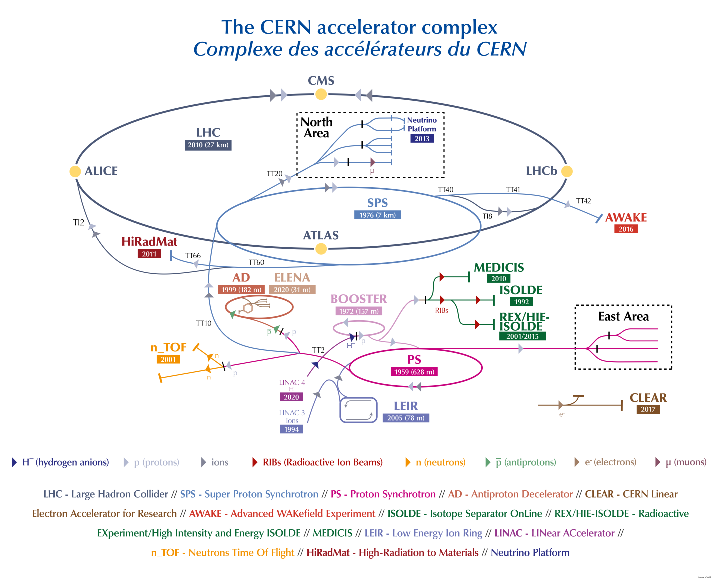
\includegraphics[width=\textwidth]{images/2-LHC-ATLAS/accelerator_complex.pdf}
\caption{An overview of the CERN accelerator complex \cite{CERN:2012:accelerators}. The LHC is fed by a series of accelerators starting with Linac4. Next are the Proton Synchrotron Booster, the Proton Synchrotron, and finally the Super Proton Synchrotron which injects protons into the LHC.}
\label{fig: accelerator-complex}
\end{figure}



%-------------------------------------------
%	Chapter 2: ATLAS
%-------------------------------------------
\section{The ATLAS Experiment}
\label{atlas-section}

\subsection{The ATLAS Detector}
The ATLAS\footnote{\textbf{A} \textbf{T}oroidal \textbf{L}HC \textbf{A}pparatu\textbf{S}.} detector is one of two general-purpose detectors in operation at the LHC \cite{PERF-2007-01}. The experiment aims to make Standard Model precision measurements and test Beyond Standard Model (BSM) theories. In total, the detector is a 44m long cylinder with a diameter of 25m and weighs over 7000 tonnes, shown in Figure \ref{fig: atlas-detector}. The detector’s geometry is cylindrical consisting of a central barrel and two end-caps to ensure forward physics coverage and hermeticity. The ATLAS detector is comprised of specialised sub-detectors, orientated coaxially around the nominal interaction point at the centre of the detector. 

\begin{figure}[htb!]
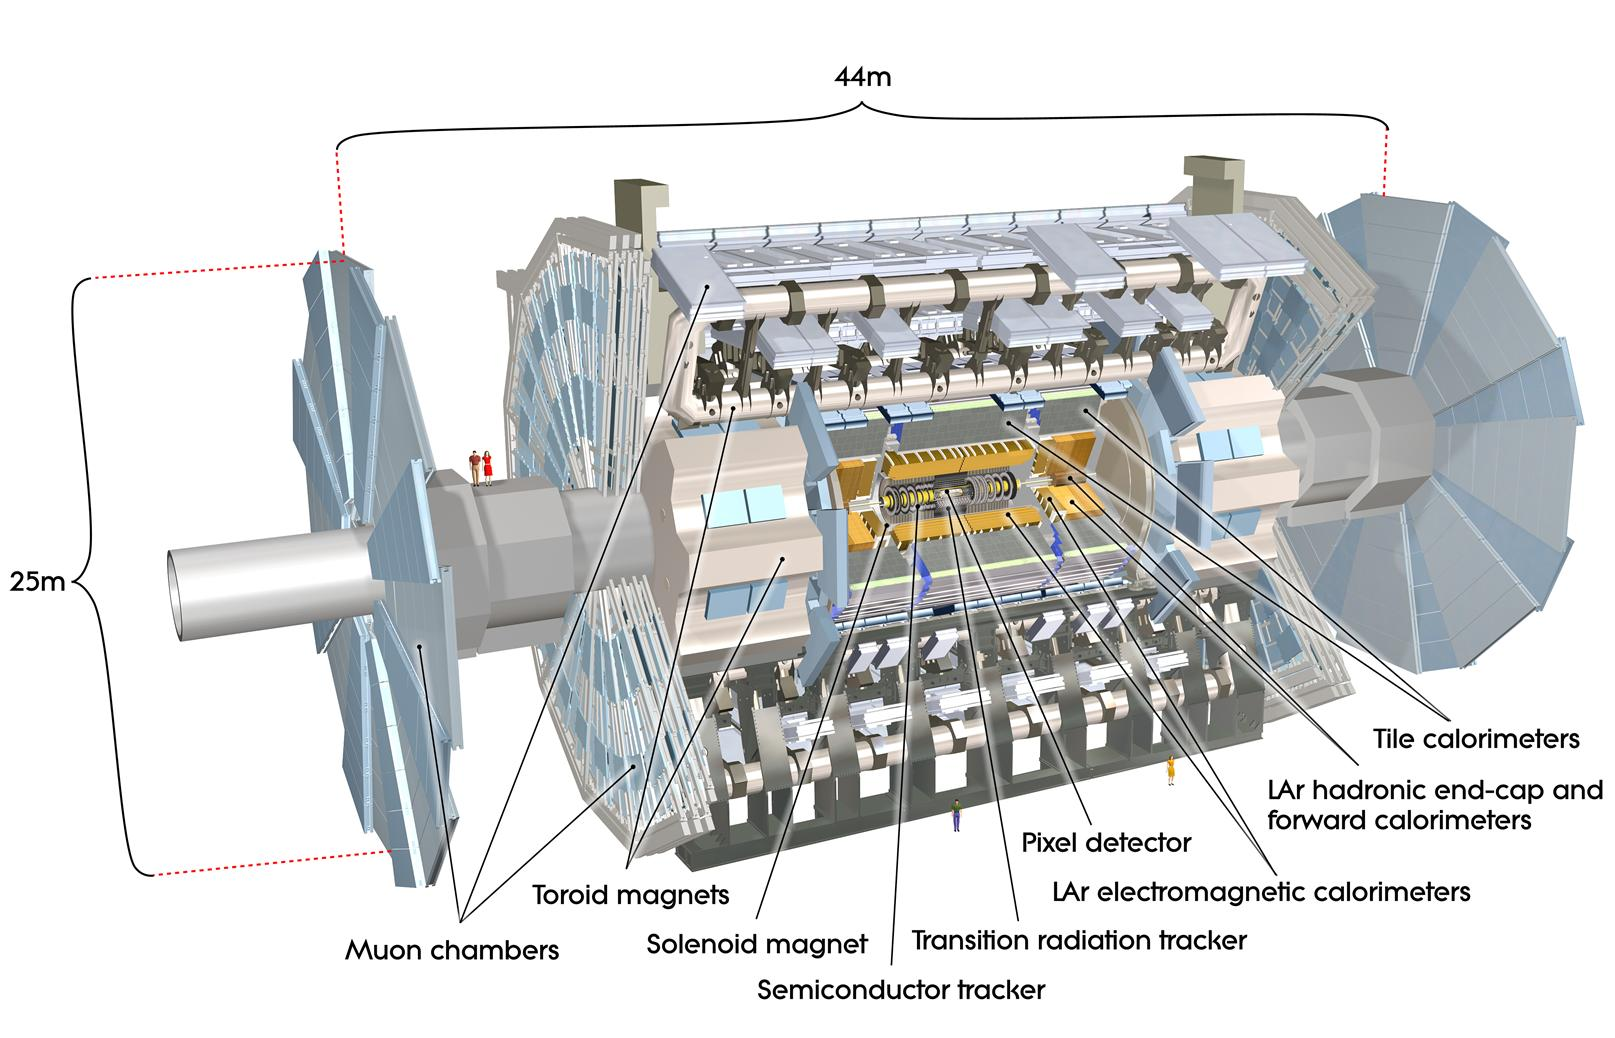
\includegraphics[width=\textwidth]{images/2-LHC-ATLAS/atlas_detector.jpg}
\caption{A 3D model of the entire ATLAS detector \cite{Jon-And:1237407}. Cutouts to the centre of the detector reveal the different sub-detectors which are arranged in concentric layers around the nominal interaction point.}
\label{fig: atlas-detector}
\end{figure}

In order of increasing radial distance, the ATLAS sub-detectors comprise of the inner detector described in Section \ref{inner-detector}, the electromagnetic and hadronic calorimeters, and the outermost muon spectrometer. 

More comprehensive details of the calorimeters and muon spectrometer can be found in the Technical Design Report (TDR) for the ATLAS detector \cite{inner-detector-TDR}. Since the work in this thesis pertains to tracking, particular attention is given to the Inner Detector which houses the tracking systems of the ATLAS detector. In Section \ref{coordinate-system} the coordinate system used at ATLAS and definitions for frequently occurring quantities are also provided.



%-------------------------------------------
%	Chapter 2: The Inner Detector
%-------------------------------------------
\subsection{The Inner Detector}
\label{inner-detector}

The inner-detector system (ID) provides high-resolution charged particle trajectory tracking in the range $ \lvert \eta \rvert < 2.5$. The ID is immersed in a 2 T axial magnetic field, produced by a superconducting solenoid magnet, which enables the measurement of particle momentum and charge. The inner detector is made up of several sub-systems shown in Figs. \ref{fig:atlas-id-run1} and \ref{fig:atlas-id-run2}. Each sub-system contains specialised hardware and contribute towards a full track reconstruction. 

\begin{figure}[!htbp]
  \centering
  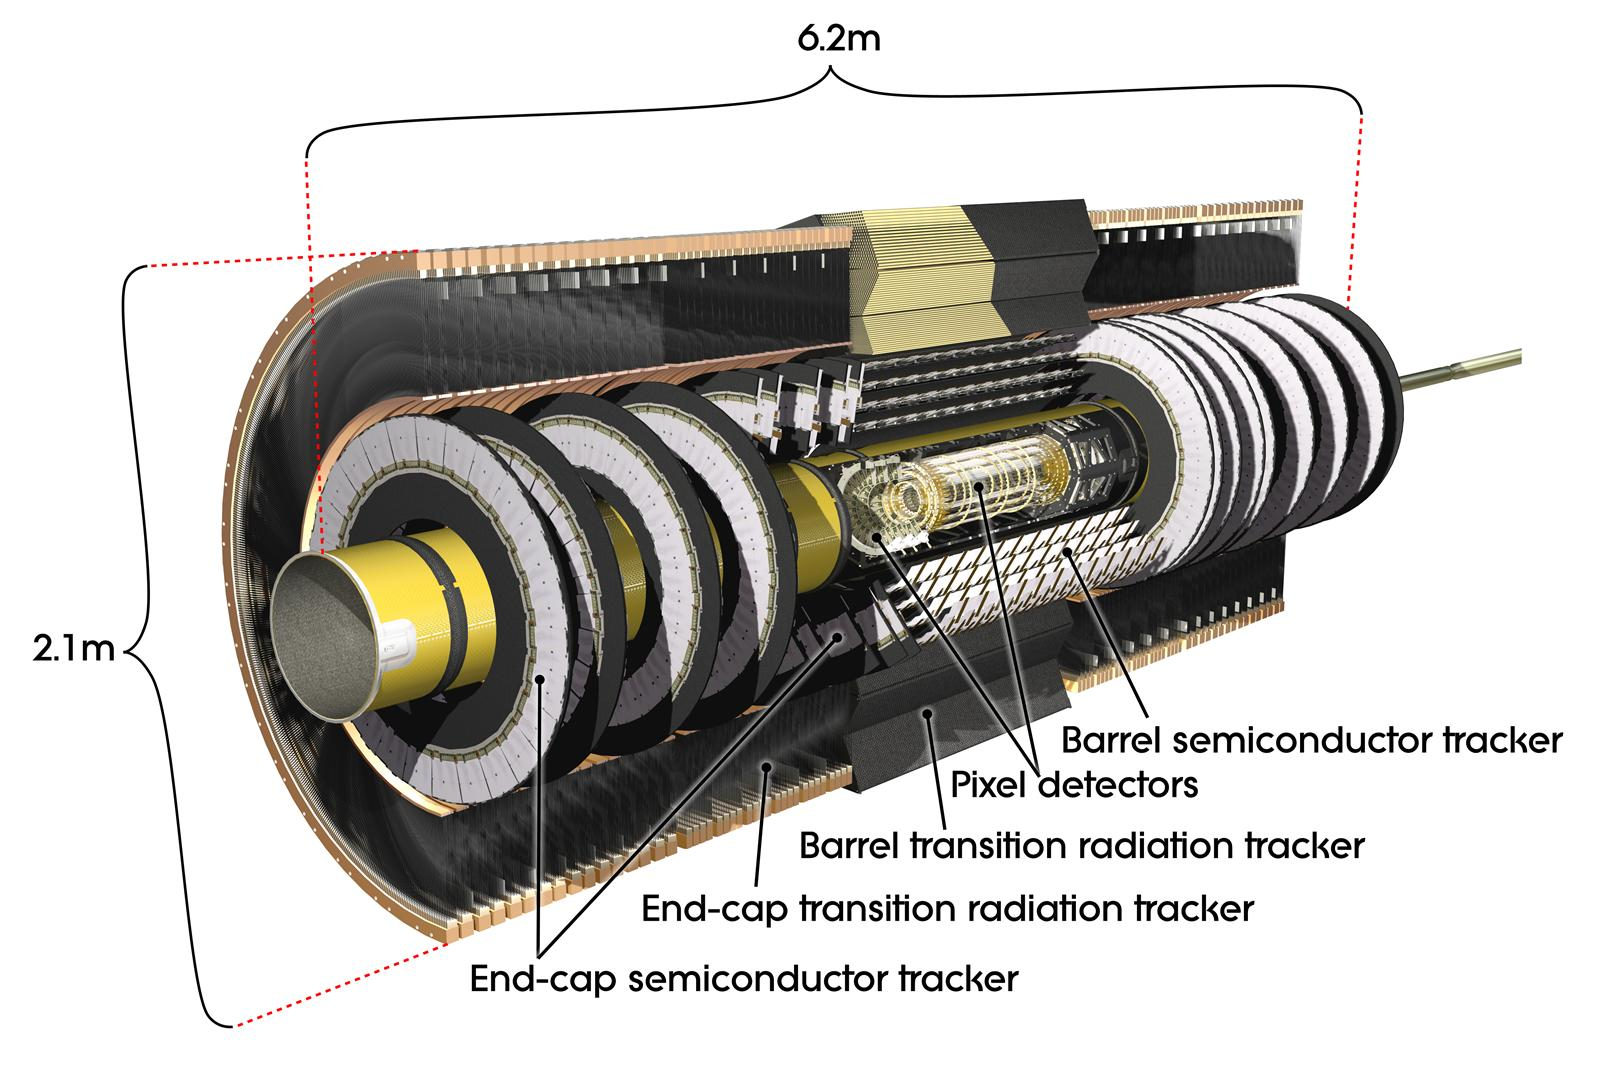
\includegraphics[width=0.75\textwidth]{images/2-LHC-ATLAS/atlas_id.jpg}
  \caption{
    A 3D model of the ATLAS ID, made up of the pixel and SCT sub-detectors, showing the barrel layers and end-cap disks \cite{atlasid}.
  }
  \label{fig:atlas-id-run1}
\end{figure}

\begin{figure}[!htbp]
  \centering
  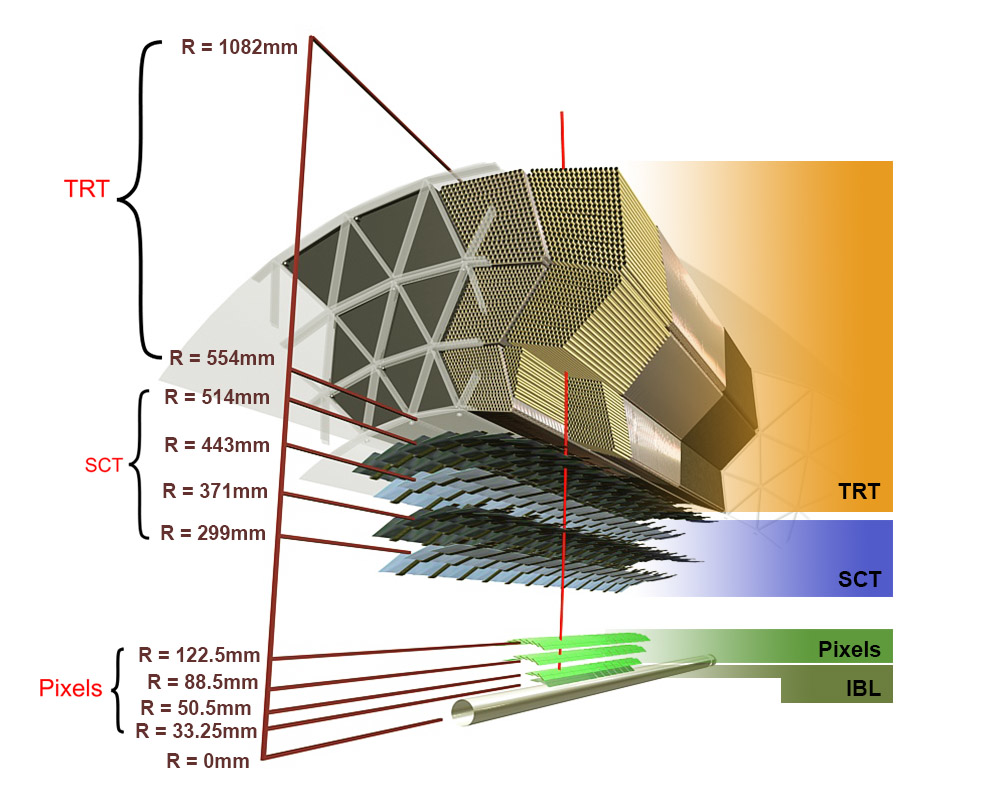
\includegraphics[width=0.75\textwidth]{images/2-LHC-ATLAS/atlas_id_xs.png}
  \caption{
    A cross-sectional view of the ATLAS ID, with the radii of the different barrel layers shown \cite{atlastrackingdocs}.
  }
  \label{fig:atlas-id-run2}
\end{figure}

The innermost silicon pixel detector \cite{pixel} provides high-granularity measurements covering the vertex region and typically provides four spacepoint measurements per track. The silicon pixel detector is comprised of four cylindrical barrels at increasing radii from the beamline, and four end-cap disks on each side. The innermost barrel layer is the insertable B-layer (IBL), which was installed before Run 2 \cite{ATLAS-TDR-19,PIX-2018-001} and lies approximately just 33mm from the beam axis. The second-to-innermost layer is often referred to as the B-layer. The pixel detector was initially constructed with 80 million readout channels, with the IBL providing an additional 12 million \cite{ibl}. The specification of the pixel detector determines the impact parameter resolution and the ability to reconstruct primary and secondary vertices. Individual pixels are 50 $\mu$m in the transverse direction $(r,\phi)$ (see Section \ref{coordinate-system} for the ATLAS coordinate system) and 400 $\mu$m in the longitudinal $z$ direction (250 $\mu$m for the IBL). 

The pixel detector is followed by the silicon microstrip tracker (SCT), which usually provides a further four spacepoint measurements per track. These silicon detectors are complemented by the Transition Radiation Tracker (TRT), which enables radially extended track reconstruction up to $ \lvert \eta \rvert = 2.0$.

The current ID has various limitations that hinder its performance as the LHC machine is upgraded. Radiation damage and high detector occupancy result in the requirement for a full replacement of the ID after Run-3 with the new ITk \cite{pileup,itk-strip}. One significant change in the detector layout is that the ITk will consist only of silicon detectors, replacing the TRT, and extend to a 1m radius, whereas the current SCT outer layer extends only to 60cm. The acceptance of the detector will be increased such that that the strip detector covers a range of $ \lvert \eta \rvert = 2.7$ with the pixel detector extending the range to $ \lvert \eta \rvert = 4.0$.

%Outside of the pixel detector, the SCT measures charged particles at an intermediate distance from the collision point and improves the determination of vertex position and track momentum. The SCT consists of four barrel layers and nine end-cap layers on each side. The outermost section of the ID, the TRT, is used for the identification of charged particles and consists of drift tubes that are filled with a mixture of Xe, CO2 and O2, and contain a central gold-plated tungsten wire. When charged particles traverse the TRT, the gas inside the straws is ionised and the free electrons drift towards the wire and are amplified and then read out. In addition, transition radiation provides information on the particle type that passed through the tracker.


%-------------------------------------------
%	Chapter 2: TDAQ
%-------------------------------------------
\subsection{The Trigger}
The 25ns bunch spacing used over the course of Run 2 corresponds to a bunch-crossing or event rate of 40MHz (see Table \ref{tab:lhc-runs}). If the full information for the detector was written out for each event, this would correspond to the generation of 60TB of data each second. This is more than can be feasibly for the read out from the hardware, the processing and storage of the data. This requires the use of a trigger system which quickly makes a decision about whether or not an event is potentially interesting and should be kept for further analysis. The trigger system is comprised of two levels which search for signs of electrons, muons, taus, photons and jets, as well as events with large total or missing transverse energy. The hardware-based Level-1 (L1) trigger uses coarse information from the calorimeters and muon spectrometer to accept events at an average rate of 100 kHz approximately 2.5 $\mu$s after the event. After the L1 trigger, the software-based High Level Trigger (HLT) makes use of 40,000 CPU cores to make a final selection on surviving events, using full granularity detector information in approximately 200ms. The final event read-out rate is approximately 1.2 kHz, corresponding to 1.2 GBs$^{-1}$ of permanent data storage. More information is provided in \cite{TRIG-2016-01}.


%-------------------------------------------
%	Chapter 2: Inner Detector Trigger
%-------------------------------------------
\subsubsection{The Inner Detector Trigger}

The ability of the ATLAS trigger system to process information from the ID to reconstruct particle trajectories is an essential requirement for the efficient triggering of physics objects. The ID trigger must therefore be able to reconstruct tracks with high efficiency across the entire range of possible physics signatures, as well as handle the rate reduction in the HLT. This challenge is exacerbated by the very high track and hit multiplicities in the ID that arise from the large pile-up. 

The ID trigger is designed to perform fast online track and vertex reconstruction using measurements from the ID. For Run 2, the ID trigger tracking is performed in two steps; the first algorithm handles trigger specific pattern recognition and seeded track finding to generate medium quality tracks as quick as possible. This is collectively known as the \textit{Fast Track Finder} (FTF) algorithm \cite{Penc:2104217, Grandi:2624768}. This step is followed by the \textit{Precision Tracking} (PT) which relies heavily on offline tracking algorithms \cite{T_Cornelissen_2008} improving their quality while applying tighter requirements. 



%-------------------------------------------
%	Chapter 2: Coordinate system
%-------------------------------------------
\subsection{Coordinate System and Collider Definitions}
\label{coordinate-system}

%% based on https://twiki.cern.ch/twiki/bin/view/AtlasProtected/PubComCommonText

The origin of the coordinate system used by ATLAS is the nominal interaction point in the centre of the detector. As shown in \ref{fig:atlas-coord-system}, the z-axis points along the direction of the beam pipe, while the x-axis points from the interaction point to the centre of the LHC ring, and the y-axis points upwards.
The transverse plane lies in $x$-$y$ while the longitudinal plane lies along the z-axis. A cylindrical coordinate system with coordinates ($r$,$\phi$) is used in the transverse plane, where $r$ is the radius from the origin and $\phi$ is the azimuthal angle around the z-axis.

\begin{figure}[!htbp]
  \centering
  % Author: Izaak Neutelings (June 2017)
% taken from https://tex.stackexchange.com/questions/159445/draw-in-cylindrical-and-spherical-coordinates
% Licensed under CC Attribution-Share Alike 4.0 International  https://creativecommons.org/licenses/by-sa/4.0/
% Original source https://wiki.physik.uzh.ch/cms/latex:example_spherical_coordinates
% Modifications by Giles Strong (March 2020):
% 1. Removal of some header code
% 2. Changing theta to eta
% 3. Addition of mountains
% 4. Changed "\draw[dashed,red] (O)  -- (Pxy);" to "\draw[->] (O)  -- (Pxy) node[right] {$p_t$};"
% Modifications by Giles Strong (April 2020):
% 1. Removal of Jura mountains
% 2. Rotated to be in terms of ATLAS coordinate system
% 3. Resized labels for the detectors

\tikzset{>=latex} % for LaTeX arrow head

\tdplotsetmaincoords{76}{45} % to reset previous setting 75 50
    \begin{tikzpicture}[scale=3.3,tdplot_main_coords,rotate around x=90]
    
    % variables
    \def\rvec{1.2}
    \def\thetavec{40}
    \def\phivec{70}
    \def\R{1.1}
    \def\w{0.3}
    
    % axes
    \coordinate (O) at (0,0,0);
    \draw[thick,->] (0,0,0) -- (1,0,0) node[below left]{$x$};
    \draw[thick,->] (0,0,0) -- (0,1,0) node[below right]{$y$};
    \draw[thick,->] (0,0,0) -- (0,0,1) node[below right]{$z$};
    \tdplotsetcoord{P}{\rvec}{\thetavec}{\phivec}
    
    % vectors
    \draw[->,red] (O) -- (P) node[above left] {$\vec{p}$};
    \draw[->] (O)  -- (Pxy) node[right] {$p_T$};
    \draw[dashed,red] (P)  -- (Pxy);
    \draw[dashed,red] (Py) -- (Pxy);
    
    % circle - LHC
    \tdplotdrawarc[thick,rotate around x=90,black!70!blue]{(\R,0,0)}{\R}{0}{360}{}{}
    
    % compass - the line between CMS and ATLAS has a ~12° declination (http://googlecompass.com)
    %\begin{scope}[shift={(1.1*\R,0,1.65*\R)},rotate around y=12]
    %    \draw[<->,black!50] (-\w,0,0) -- (\w,0,0);
    %    \draw[<->,black!50] (0,0,-\w) -- (0,0,\w);
    %    \node[below right,black!50,scale=0.6] at (\w,0,0) {N};
    %\end{scope}
    
    % nodes
    \node[right] at (\R,0,0) {LHC};
    \fill[radius=0.8pt,black!20!red]
        (O) circle node[left=4pt,below=5pt] {ATLAS};
    \draw[thick] (0.02,0,0) -- (0.5,0,0); % partially overdraw x-axis and CMS point
    \fill[radius=0.8pt,black!20!blue]
        (2*\R,0,0) circle
        node[right=4pt,below=2pt,scale=0.7] {CMS};
    \fill[radius=0.8pt,black!10!orange]
        ({-\R*sqrt(2)/2+\R},0,{-\R*sqrt(2)/2}) circle % 45 degrees from ATLAS
        node[left=2pt,below=2pt,scale=0.7] {ALICE};
    \fill[radius=0.8pt,black!60!green]
        ({-\R*sqrt(2)/2+\R},0,{\R*sqrt(2)/2}) circle % 45 degrees from ATLAS
        node[below=6pt,right=3pt,scale=0.7,anchor=north east] {LHCb};
    
    % arcs
    \tdplotdrawarc[->]{(O)}{0.2}{0}{\phivec}
        {above=2pt,right=-1pt,anchor=mid west}{$\phi$}
    \tdplotdrawarc[->,rotate around z=\phivec-90,rotate around y=-90]{(0,0,0)}{0.5}{0}{\thetavec}
        {anchor=mid east}{$\eta$}
\end{tikzpicture}
  \caption{
    The coordinate system used at the ATLAS detector, showing the locations of the four main experiments located at various points around the LHC. The 3-vector momentum $p_{T} = (p_x, p_y, p_z)$ is shown by the red arrow. Reproduced from \cite{Strong:2020mge}.
  }
  \label{fig:atlas-coord-system}
\end{figure}

%The pseudorapidity is defined in terms of the polar angle $\theta$ as $\eta = -\ln \tan(\theta/2)$.

The polar angle $\theta$ is commonly specified in terms of the pseudorapidity $\eta$, defined as
%
\begin{equation}\label{eq:pseudorap}
  \eta = - \ln \left[ \tan \left( \frac{\theta}{2} \right) \right] .
\end{equation}
%
The pseudorapidity is a convenient quantity to work with as differences in $\eta$ are invariant under Lorentz boosts. In addition, particle production is constant as a function of $\eta$.

Additionally, the transverse plane is often used to describe the kinematics of collisions, where the transverse momentum $p_{T}$ of an object is the sum in quadrature of its momenta components.
%
\begin{equation}\label{eq:pt}
  p_T = \sqrt{ {p_x}^2 + {p_y}^2 }
\end{equation}



%-------------------------------------------
%	Chapter 2: Motivation for Hi-Lumi LHC
%-------------------------------------------
\section{Motivation for the HL-LHC}
\label{hi-lumi}

% - the physics motivation to increase the luminosity - brief 

The HL-LHC is an upgrade of the LHC to achieve higher precision measurements by using instantaneous luminosities a factor of five larger than the nominal value. This will enable the detector's discovery power and exploration potential to significantly improve. Initially, the luminosity will be increased to $5 \times 10^{34} cm^{−2}s^{−1}$, and subsequently increased up to $7.5 \times 10^{34} cm^{−2}s^{−1}$ by the mid-2030s. As a result, the experiment's data sample will enlarge by one order of magnitude compared with the baseline programme.

Since the discovery of the Higgs boson at the ATLAS and CMS experiments \cite{ATLAS-HIGGS, CMS-HIGGS} in 2012, the study of the Higgs sector has greatly expanded to include many precision measurement analyses, predictions from theory and searches for rare production and decay processes. One important question to answer is whether the observed Higgs is that predicted from the electroweak symmetry breaking mechanism \cite{ewsb} or if it is, in fact, the first signal in some Beyond Standard Model (BSM) physics. With the accumulated data so far, the identity of the Higgs boson is consistent with SM predictions and all measurements are proportional to the particles’ masses, but higher-precision measurements of these couplings could illuminate any potential discrepancies from prediction. Further information on the Higgs mechanism can be found in \cite{Bednyakov_2008}.

%With the accumulated data so far, the identity of the Higgs boson is consistent with SM predictions and all measurements are confined to the couplings of the Higgs to SM particles, which are proportional to the particles’ masses, but higher-precision measurements of these couplings could illuminate any potential discrepancies from prediction.

In general, precision measurements of the Higgs sector provide indirect probes to just about any extension of the SM. There are many theoretical particles predicted by various BSM scenarios that can also be searched for in the HL-LHC. One set of such scenarios falls under the title of Super-symmetry (SUSY) \cite{supersym}, which predicts super-partners belonging to every fermion and every boson. Direct dark matter searches can also be probed at higher mass scales, and new detector upgrades will facilitate searches for long-lived exotic particles. Additionally, BSM physics can be further probed through rare \textit{b} and \textit{c} hadron decays that may be measured using the increased integrated luminosity \cite{wg-bsm}.

The physics programme offered by the HL-LHC is vast \cite{big-report}; a detailed description of the project and its technological and operational challenges is provided in the HL-LHC Preliminary Design Report \cite{Apollinari:2116337}. The programme would deliver an unprecedented potential for new physics discoveries and incredibly high-precision SM measurements. However, the promising plan for the future is accompanied by many technical challenges that each of the experiments face. The increased luminosity results in greater pile-up, which results in drastically higher detector occupancy and radiation levels. In the case of ATLAS, Figure \ref{fig:pileup-walltime} shows the projected evolution of compute usage from 2020 until 2036 under different R\&D scenarios. The expected pile-up levels during the HL-LHC are around $\langle \mu \rangle$ = 200, demonstrating the need for upgrades to both the detector and algorithmic designs.

\begin{figure}[!htbp]
  \centering
  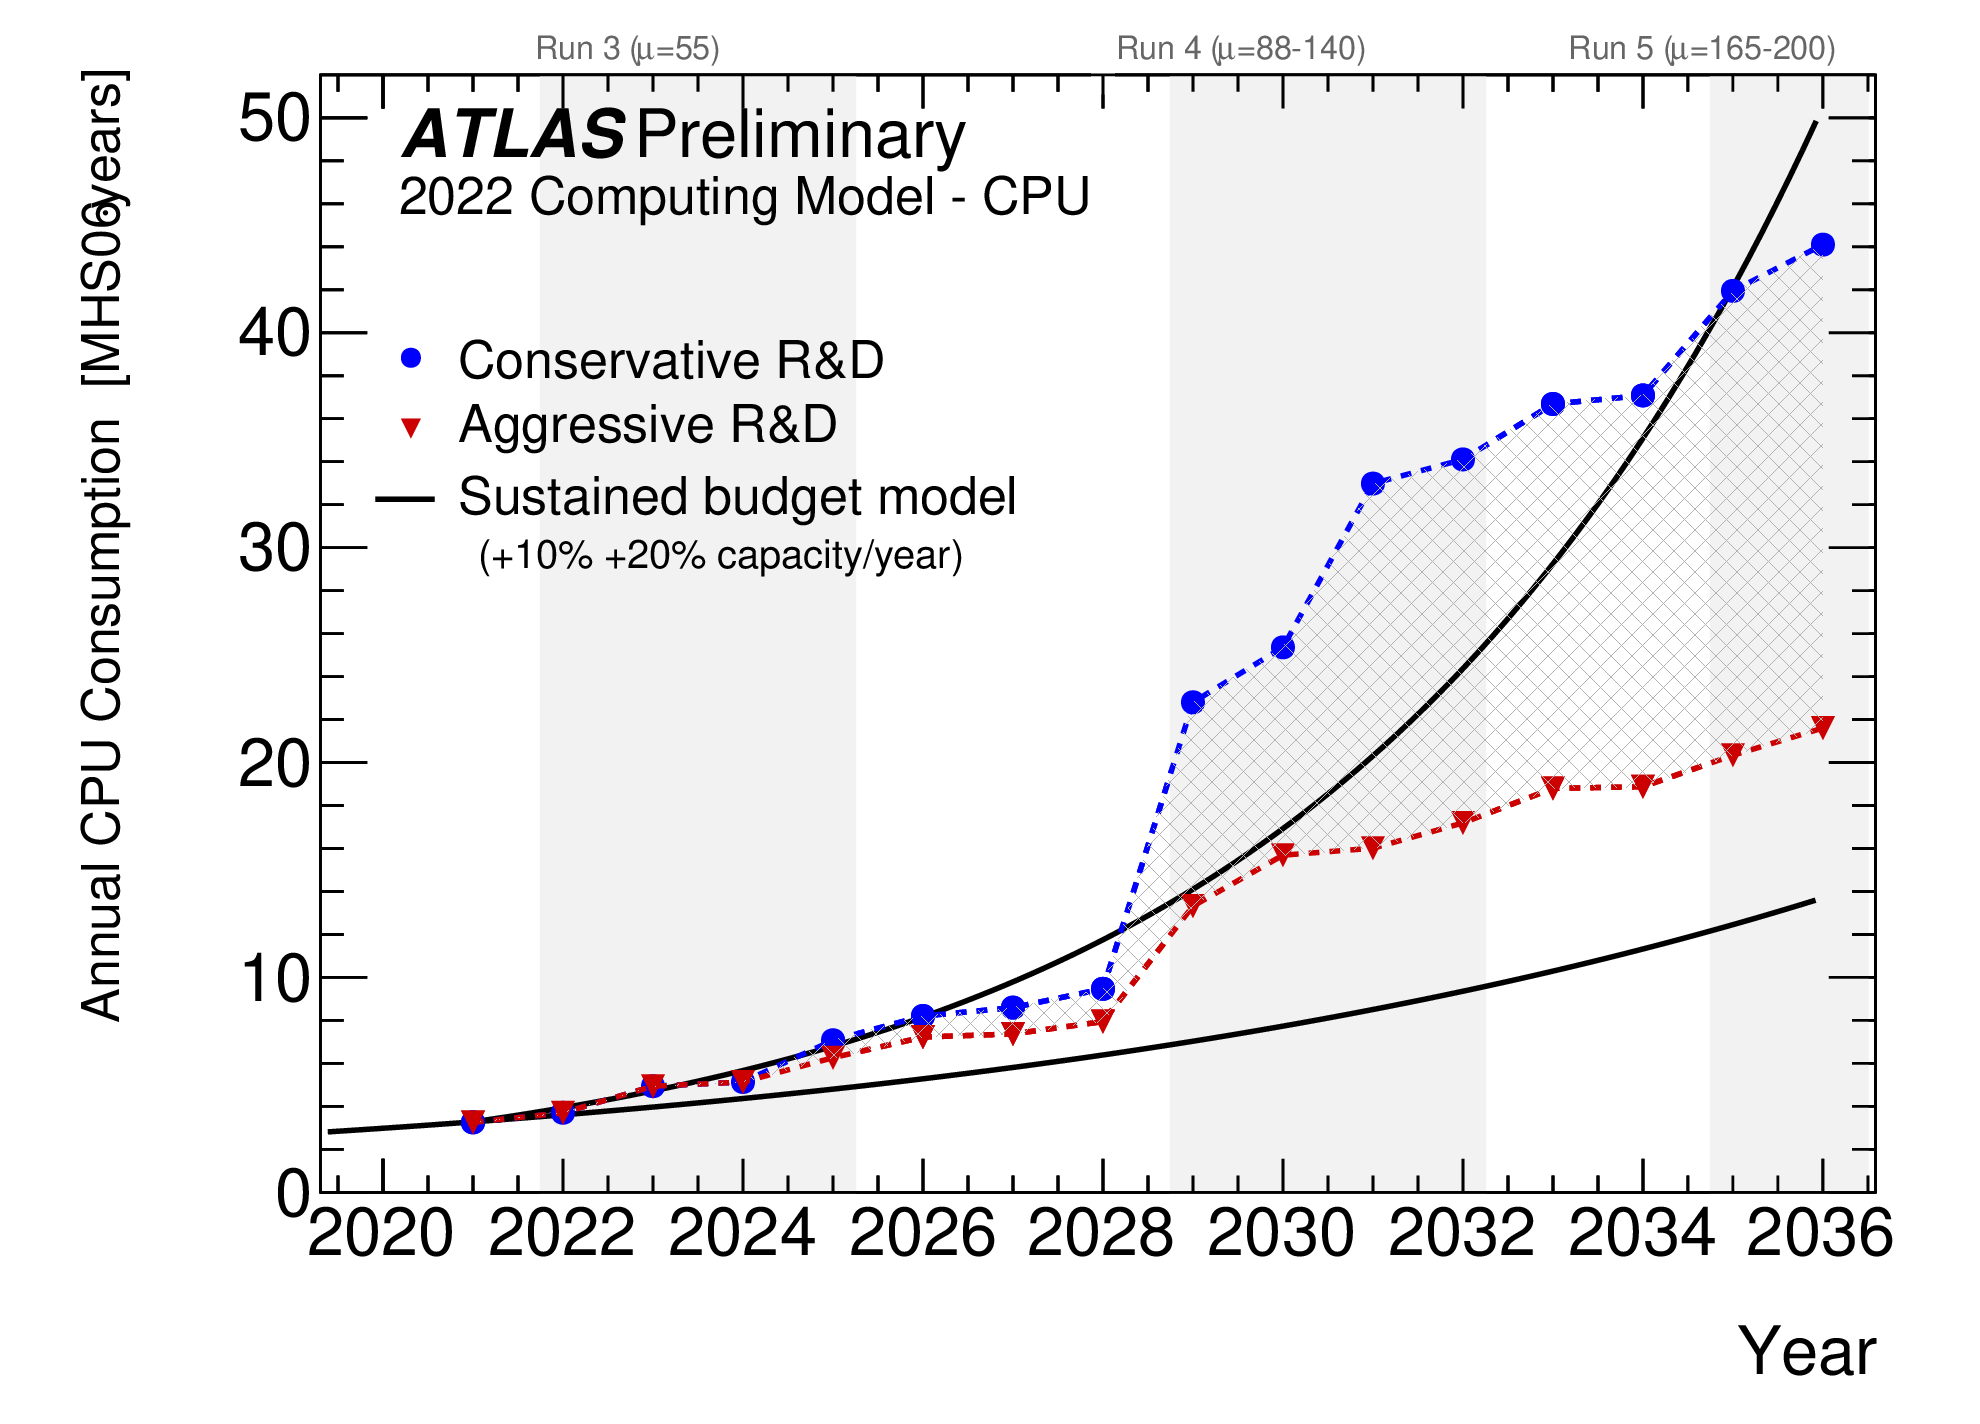
\includegraphics[width=0.8\textwidth]{images/2-LHC-ATLAS/computing-model.png}
  \caption{
    Projected evolution of compute usage under the conservative (blue) and aggressive (red) R\&D scenarios. The grey hatched shading between the red and blue lines illustrates the range of resource consumption if the aggressive scenario is only partially achieved. The black lines indicate the impact of sustained year-on-year budget increases and improvements in new hardware, that together amount to a capacity increase of 10\% (lower line) and 20\% (upper line). The vertical shaded bands indicate periods during which ATLAS will be taking data \cite{Collaboration:2802918}.
  }
  \label{fig:pileup-walltime}
\end{figure}

%In the case of ATLAS, Figure \ref{fig:pileup-walltime} shows how the reconstruction time per event increases with pile-up. The increase in time is exponential, and the expected pile-up levels during the HL-LHC are around $\langle \mu \rangle$ = 200, demonstrating the need for upgrades to both the detector and algorithmic designs in ATLAS.

%\begin{figure}[!htbp]
%  \centering
%  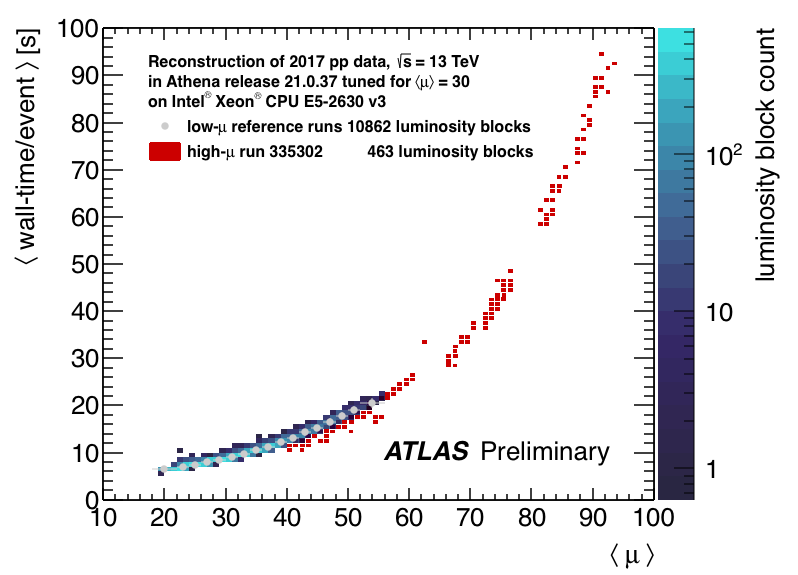
\includegraphics[width=0.8\textwidth]{images/2-LHC-ATLAS/pileup-walltime.png}
%  \caption{
%    The dependency of reconstruction wall time per event on pileup. The luminosity block count represents short intervals of data taking, in which the instantaneous luminosity is estimated, and from this the integrated luminosity derived \cite{pileup}.
%  }
%  \label{fig:pileup-walltime}
%\end{figure}

\doublespacing

%-------------------------------------------
%	Chapter 3: Track Reconstruction
%-------------------------------------------
\chapter{Track Reconstruction}
\label{chapter-3}

%H important to help show the bigger picture of my research and the motivation behind the work presented

%Successful particles physics measurements are dependent on an efficient and performant re- construction of the physics objects from the detector measurements. As a community we are always striving to run at the edge of the available detector and computation capabilities to ex- tract the maximum amount of information from the experiments. Tracking detectors are at the core of most collider experiments and track reconstruction is one of the crucial tasks in every reconstruction chain.

%Track reconstruction at its heart is a combinatorial problem, i.e. to find the measurements that originate from the same initial particle from a set of possible combinations. The created particles have a wide range of possible properties, especially different creation vertices and momenta, and their particle trajectories have non-deterministic contributions from material interactions. In combination with inhomogeneous magnetic fields and detector inefficiencies, this leads to the possibility of confusion, fake tracks, etc. . All of these effects depend strongly on the density of the measurements and thus on the collision pile-up. Consequently, with the upcoming upgrade to the High-Luminosity Large Hadron Collider (HL-LHC) the track reconstruction complexity will increase significantly.

In this chapter, track finding in silicon based detectors is presented. Section \ref{track-finding-silicon-trackers} outlines a typical workflow for track reconstruction in a multi-element silicon tracker and the parameterisation used for specifying the trajectory of charged particle tracks. Section \ref{trackml-detector} presents the TrackML detector and ML challenge; a realistic detector model used to simulate measured particle hits similar to what is expected of the HL-LHC experiment, as well as new approaches to track reconstruction that arose from the challenge. Finally, graph network architectures and track reconstruction using graph networks is presented in Section \ref{graph-networks}, as a potential solution and optimisation to the track finding problem.

%The aim of this project is to explore track finding methods utilizing a graph-based track model and graph neural networks (GNN). An ML-based algorithm will be used to predict a graph adjacency matrix given the input hit features such as a shape of a charge cluster representing a track position measurement in a silicon detector. The excitation/inhibition rules of individual GNN neurons will be designed to facilitate the “simple-to-complex” approach for “hits-to-tracks” association such that the network starts with relatively “easy” areas of an event with low hit density and gradually progresses towards more complex “hot” areas. To efficiently exploit a priori knowledge about charged particle dynamics the GNN-based algorithm will be using simplified Kalman filters as mechanisms for information propagation and track extraction. 

% first talk about graph building using the ML hit pair predictor and then talk about graph pruning/track extraction using the GNN based algorithm



%--------------------------------------------------
%	Chapter 3: Track finding in Silicon Trackers
%---------------------------------------------------
\section{Track Finding in Silicon Trackers}
\label{track-finding-silicon-trackers}

%The reconstructed trajectories of charged particles are referred to as tracks. 
%Tracks are reconstructed from the energy depositions (called hits) left by the particles as they traverse the the inner detector.


A typical workflow for track finding in a multi-element silicon tracker (such as those in ATLAS and CMS) comprises a three-stage approach; seeding, track following, and track selection, implemented in many charged particle tracking algorithms. A comprehensive introduction to ATLAS tracking is available in Ref \cite{Cornelissen:2007vba}. An overview of track reconstruction in a multi-element silicon detector is given below.

%The main sequence is referred to as ’inside-out’ track finding, involving clusterisation [17], a CPU-expensive ’track-finding’, followed by precise estimation of track parameters via ’track-fitting’.


%--------------------------------------------------
%	Chapter 3: Track Reconstruction
%---------------------------------------------------
\subsection{Track Reconstruction}
\label{track-reconstruction}

%Describe a typical workflow for track finding in a typical multi-element silicon tracker such as ATLAS and CMS. This workflow is basically a three-stage approach with the seeding, track following, and track selection implemented in the current charged particle tracking algorithms. This is precisely the right place to introduce the TrackML setup. Add that the high-lumi LHC motivates the R\&D of new track finding techniques and we need an environment for fast prototyping and testing various techniques which would allow expert from outside HEP to contribute hence the TrackML.

%This section should be all about track finding in ATLAS, including the main pipeline outlining space-point formation (clustering), track finding (combinatorics), ambiguity solving, neural network cluster splitting, pattern recognition techniques, Kalman filters etc 


\subsubsection{Space-point Formation (Clustering)}
When a charged particle traverses a silicon layer, charge can be deposited in more than one Pixel or Strip. This is due to the incident angle of the particles with respect to the sensor and also the drift of electrons inside the sensor caused by their interaction with the magnetic field. Clusters are formed by grouping together neighbouring pixels or strips. The local position of the cluster on the sensor is typically estimated using the energy-weighted mean position of the pixels (or strips) forming the cluster. The clusters are then converted into 3D space-points by a coordinate transformation, where pixel space-points are identical to pixel clusters and strip space-points are formed by combining information from two strip clusters in subsequent sensors in the SCT (or strip double layers of the ITk).

\subsubsection{Seeded Track Finding}
Space-points are used to build track seeds. Seeds are defined as a group of three space-points located in different detector layers which are geometrically compatible with being part of a track segment. A combinatorial KF is used to build track candidates by extending track seeds. The filter can create multiple track candidates per seed, with bifurcations along the track occurring when more than one compatible space-point exists in a given layer. In this way, the KF creates an excess of track candidates, which are only required to satisfy basic quality requirements. Track candidates are allowed to share hits freely (a single hit may be used by multiple track candidates). Typically, the presence of shared hits is an indication of a bad track due to the high granularity of the ATLAS tracking detectors. At this stage, there can also be a large number of incorrect hits assigned to otherwise good tracks, and large numbers of fake tracks. Fake tracks are those where the majority of associated hits do not originate from the trajectory of any one physical particle. The low quality of tracks at this stage necessitates an ambiguity resolution step, in which the highest quality tracks are selected.

\subsubsection{Track Ambiguity Resolution}

The procedure so far has created candidates with potential overlap. In the ambiguity solver of the ATLAS detector, track candidates are processed individually in descending order of a track score in an effort to resolve this overlap. The track score quantifies the likelihood of the track corresponding to the trajectory of a real particle. Scoring uses a number of variables, including the number and positions of hits, the transverse momentum of the track and the fit quality described as the $\chi^{2}$ divided by the number degrees of freedom on the track. A preference for high transverse momentum tracks promotes the successful reconstruction of the more physically interesting energetic particles, and suppresses the large number of wrong hits assigned to low momentum tracks. Ambiguity solving was introduced as part of the ATLAS New Tracking (NEWT) \cite{Cornelissen:2007vba} intended to improve track reconstruction performance in dense environments. 

\subsubsection{TRT Extension}

The successful tracks from the ambiguity solving stage are extended into the TRT if there is a valid set of matching drift circles. A subsequent track refit is performed in order to increase the precision in parameters of the reconstructed track.


%--------------------------------------------------
%	Chapter 3: Track Parameterisation
%---------------------------------------------------
\subsection{Track Parameterisation}
\label{track-parameterisation}

There are several parameterisations of tracks, but since the shape of the charged particle trajectories in a uniform magnetic field is helical, in general five parameters are required to approximate the true trajectory. One such parameterisation is known as perigee given by Eq. \ref{perigee}:

\begin{equation}\label{perigee}
\textbf{p} = (d_0, z_0, \phi, \theta, Q/p_T)
\end{equation}

The respective transverse and longitudinal impact pararameters; $d_0$ and $z_0$ specify the distance of closest approach of the trajectory of a particle to the nominal interaction point. $\phi$ is the azimuthal angle in the $x$-$y$ plane and $\theta$ is the polar angle in the $(r,z)$ plane. In fact, we often use $\cot(\theta)$ instead of $\theta$, since $\cot(\theta)$ is the inverse slope of the track. $Q/p_T$ is the inverse transverse momentum multiplied by the charge of the particle. Fig. \ref{fig:track-parameters-perigee} shows each of these parameters diagrammatically.


\begin{figure}[!htbp]
  \centering
  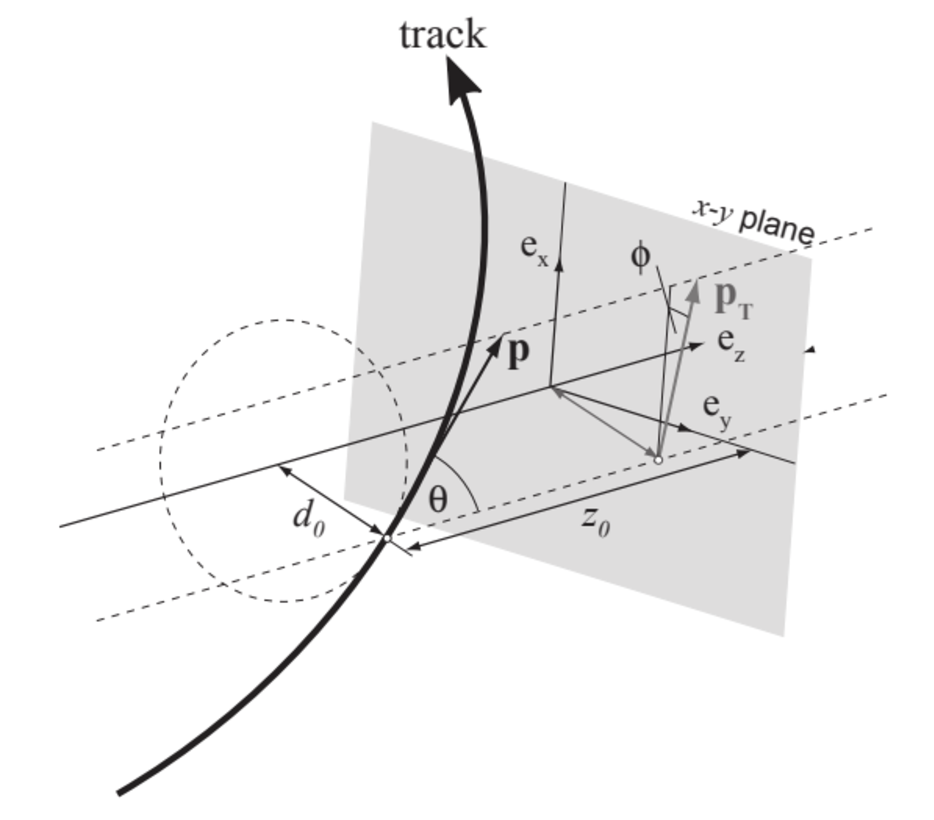
\includegraphics[width=0.75\textwidth]{images/3-track-reconstruction/track_params.pdf}
  \caption{Illustration of the perigee track parameters. Five coordinates are specified $(d_0, z_0, \phi, \theta, Q/p_T)$, defined at the track’s point of closest approach to the nominal interaction point at the origin of the coordinate system. The three-momentum \textbf{p}, transverse momentum $p_T$ and basis vectors $e_x$, $e_y$ and $e_z$ are also shown. Reproduced from Ref. \cite{atlastrackingdocs}
  }
  \label{fig:track-parameters-perigee}
\end{figure}


%--------------------------------------------------
%	Chapter 3: TrackML Model
%---------------------------------------------------
\section{The TrackML Model}
\label{trackml-detector}

As the CPU time to reconstruct particle trajectories from measurements is expected to increase faster than the projected computing resources for future detector upgrades, new approaches to pattern recognition are needed to fully exploit the discovery potential of modern silicon detectors. In order to acquire an environment for fast prototyping and developing various techniques, a realistic detector model is needed. As a result, in 2018 a tracking ML challenge was organised on the Kaggle platform; an open-source community platform for data scientists dedicated to the use of challenges as a research tool. The \textit{TrackML Particle Tracking Challenge} \cite{kaggle-trackml} was held in an effort to spark new ideas and algorithmic approaches towards track reconstruction.

The basis of the challenge is using a realistic detector model, develop an algorithm for tracking trajectories of particles using machine learning techniques. The TrackML model simulates measured particle hits similar to what is expected for a HL-LHC experiment and the corresponding data contains 8000 events to train on, where each event has up to 100,000 hits. The participants of the challenge were tasked with connecting these hits into approximately 10,000 arcs of circles, following the trajectory of particles issued from truth data from high energy proton collisions. 

There are many different approaches explored within the TrackML challenge, where the definition of a track determined the most effective approach to use. For example, for a track defined as a point-like object in a parameter space, clustering algorithms would be most appropriate. Whereas, for a track can modelled as a sequence of hits, a track following algorithm using an iterative predict and update mechanism would be most effective.

The structure of the TrackML detector is shown in Section \ref{trackml-structure}, the simulation of the model is discussed in Section \ref{trackml-simulation} and a summary of the challenge algorithms that is beneficial for this thesis is presented in Section \ref{trackml-key-findings}. The TrackML detector is also used for the development of the GNN-based algorithm; see Chapter \ref{chapter-6} for further information. More information on the TrackML challenge can be found in \cite{Amrouche_2019}.

\subsection{TrackML Detector Structure}
\label{trackml-structure}
The structure of the detector adopts a generic tracker design that takes key concepts from the existing proposals from ATLAS and CMS detectors. Many modern particle detectors include extensive silicon tracking systems arranged in thin layers of silicon sensors. The TrackML detector is very similar in structure to that of modern detectors, such as the ATLAS ITk \cite{inner-detector-TDR} being built for the HL-LHC era. It uses a cylinder-like geometry in the central regions and a disk-like geometry in the forward regions. The full TrackML detector geometry is shown in Figure \ref{fig:trackml-detector-image}. 


\begin{figure}[!htbp]
  \centering
  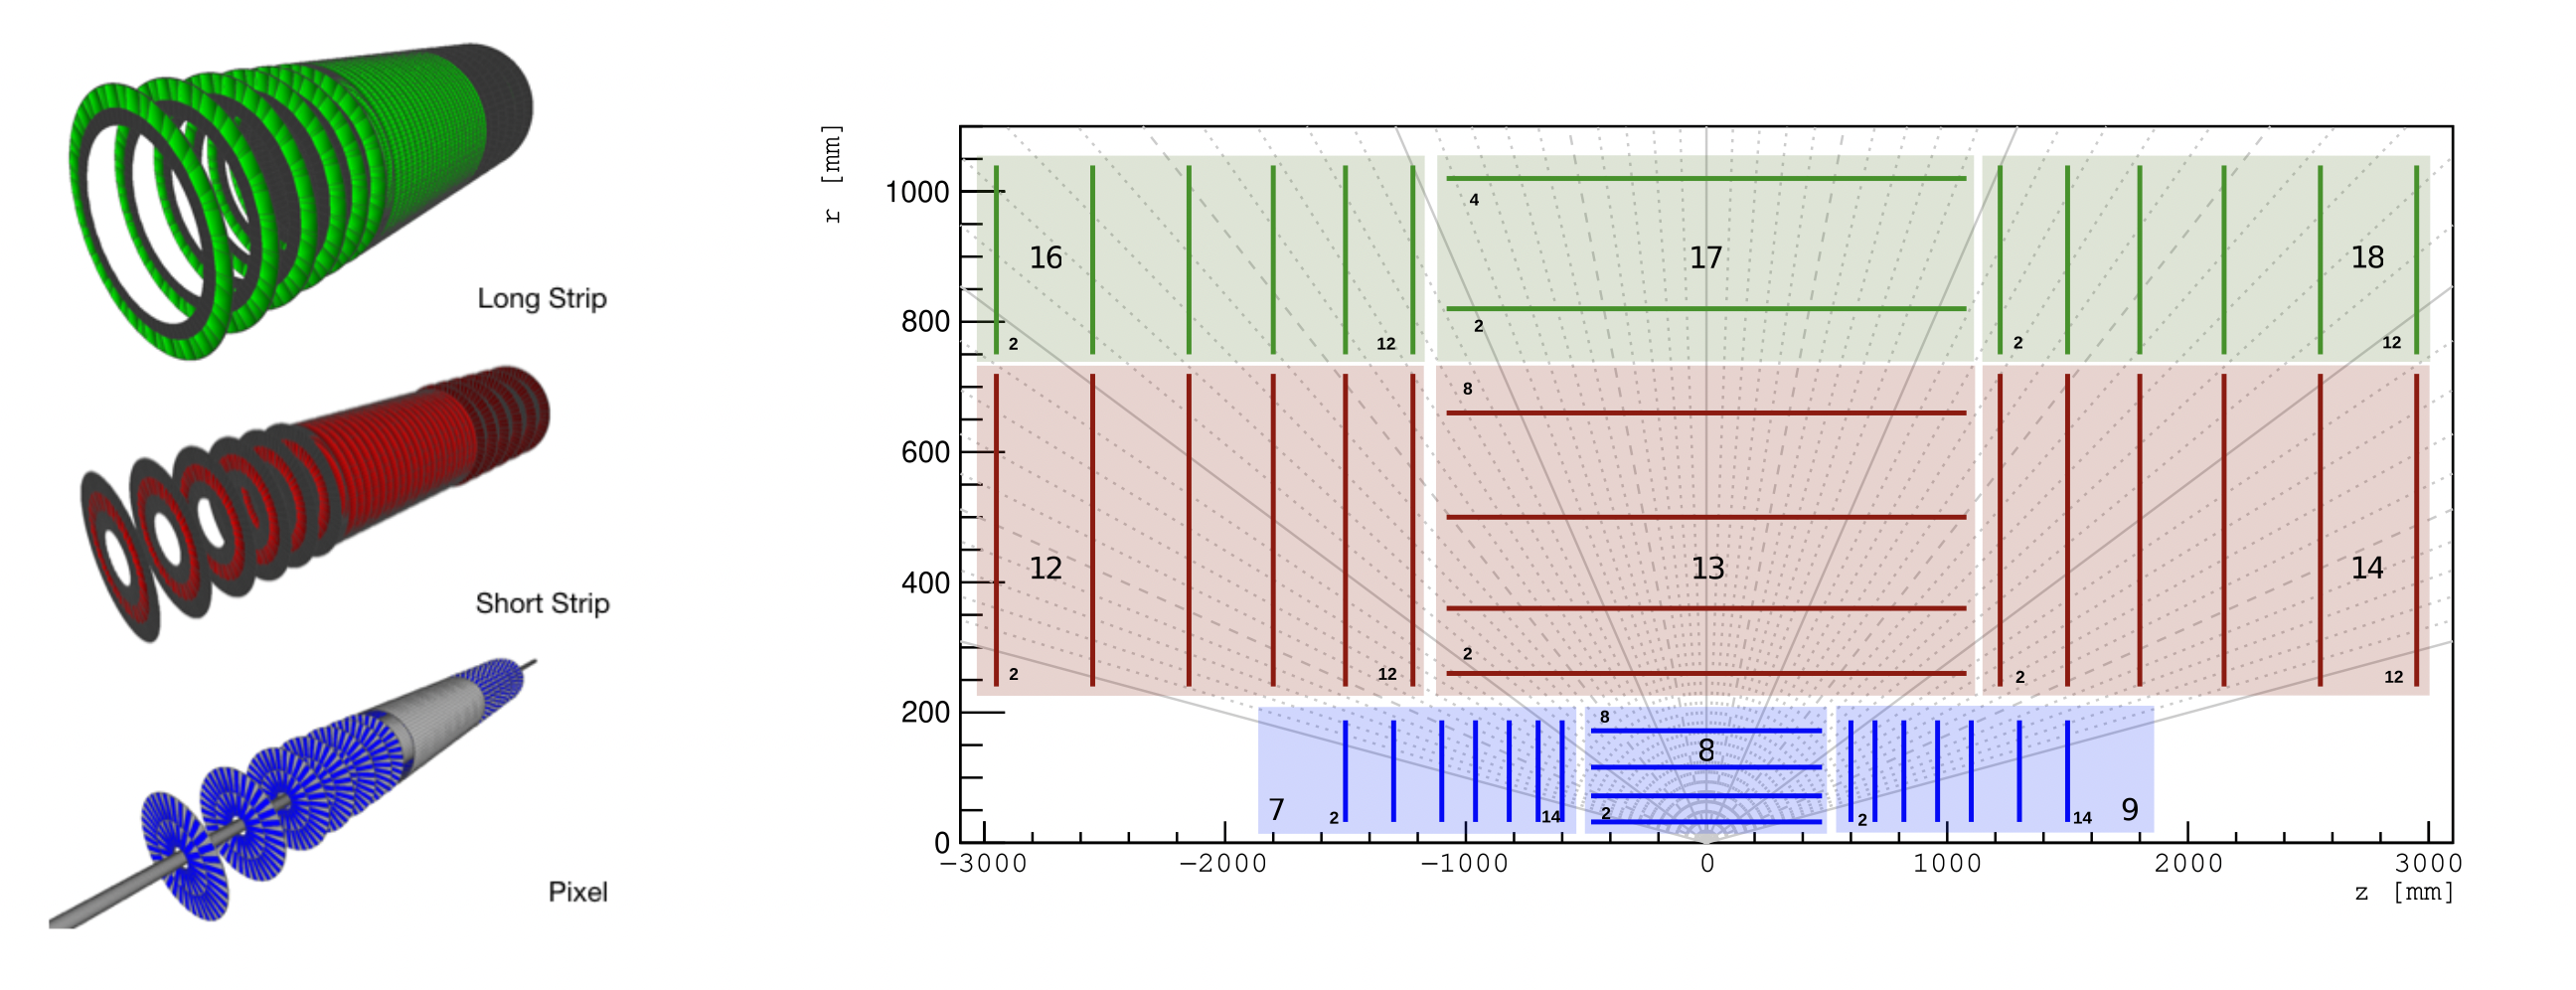
\includegraphics[width=\textwidth]{images/3-track-reconstruction/trackml-detector.png}
  \caption{
    Detector layout for the virtual TrackML detector. On the left the three major sub-detectors, pixel, short strips, and long strips, are shown separately. On the right, a schematic of the full layout and its coverage along the radial and longitudinal dimensions as well as in the $ \lvert \eta \rvert$ direction is shown. The different colors represent the different sub-detectors while the marked numbers are the internal volume and layer identifiers.
  }
  \label{fig:trackml-detector-image}
\end{figure}



The detector is split into three separate sub-detectors that differ in spatial resolution and passive material. The innermost sub-detector is a Pixel detector with a spatial resolution of 50$\mu$m $\times$ 50$\mu$m and further out two different strip detectors with short 80$\mu$m × 1200$\mu$m and long strips 0.12 mm $\times$ 10.8 mm are placed. Each detector includes realistic module geometries with placement and overlap chosen to yield a hermetic coverage up to $\lvert \eta \rvert$ = 3. The particle beams collide on the $z$-axis around z = 0. This is the centre of collision and also the centre of the detector. The TrackML detector is also organized into groups of layers, called \textit{volumes}, which are identified by a volume number. The Pixel detector is represented by volumes 7, 8 and 9.

%ITK: There is no reason to believe the more complex geometry would lead to radically different algorithms

%The TrackML detector also shares several interesting features with the ATLAS detector, for example its solenoid parameters are the same and ....

%Instead of using the proposed upgrade tracker designs of either ATLAS or CMS we opted to design a generic tracker design that takes the key concepts from the existing proposals. This avoids issues of private collaboration information or artefacts and allows a challenge that is more separated from the particular design choices made by each experiment.

% -------------------------------
%More details in the documents on the TrackML competition:
%https://hal.inria.fr/hal-01745714/document
%https://arxiv.org/pdf/1904.06778.pdf
% ------------------------------


\subsection{Event Simulation}
\label{trackml-simulation}
%10.1051_epjconf_201921406037.pdf
The particle content of the collisions is generated using the Pythia 8 event generator \cite{pythia-8}. A hard Quantum Chromodynamic (QCD) interaction that generates a $t\bar{t}$-pair is used as the signal. An additional 200 soft QCD interactions are overlayed to simulate the expected pile-up conditions at the HL-LHC. Charged particles are propagated through the detector using a fast detector simulation based on the ACTS software \cite{Gumpert_2017}. A non-homogeneous magnetic field is used, similar to the one in the ATLAS experiment, and material interactions, i.e. multiple scattering, energy loss, or hadronic interactions, are simulated using parametric models. Only tracks with a transverse momentum above 150 MeV are propagated. Tracks below this momentum threshold are typically not considered by the HL-LHC experiments.

% top quark decays: https://en.wikipedia.org/wiki/Top_quark

\subsection{Challenge Summary and Outlook}
\label{trackml-key-findings}

\subsubsection{Review of Submitted Algorithms}
The TrackML competition exposed a diverse range of ML approaches, where accuracy and throughput was used to categorise the best algorithms for track reconstruction. The performance of the algorithms are evaluated using track purity and particle purity, for tracks originating from primary particles produced in the actual pp collisions. The purity is defined as follows; each track is matched with the ground truth majority particle sharing with it the greatest hit number, $N_{truth}$. The ratio of $N_{truth}$ to the number of hits of the reconstructed track, $N_{hits}$, defines the track purity, while the ratio of $N_{truth}$ intersection to the number of hits of the underlying particle, $N_{phits}$, defines particle purity. The quality of the top performing algorithms were analyzed in further detail. It was found that methods based on track following techniques are highly effective at reconstructing tracks globally with high purity, in comparison with clustering based approaches. 

Amongst the top ranking solutions, the developed algorithms were highly inspired from traditional track following approaches, such as the procedure outlined in Section \ref{track-reconstruction}. The winning algorithm is based on a modular track following strategy, where the definition of a track is given by a sequence of hits. It begins with seed generation selected from hit pairs (doublets) in the innermost layers of the detectors. A logistic regression classifier is trained on doublet features and allows to reduce the number of fake seeds. These doublets are then extended to triplets via a further logistic classifier trained on triplet features. Track following is then implemented using a helix extrapolation and track ambiguity resolution is executed to remove polluting hits.

% Tracks are then consolidated by taking into account any hits located on overlapping modules if they are closer than a threshold.

Another high-ranked algorithm is based on training a multi-layered perceptron (MLP) to predict any two hits that are connected to the same track, where the definition of a track is the same as above. All pairs of hits were considered and 27 features were constructed from its quantities. A neural network model composed of multiple wide dense layers is trained to predict the probability of the pair to be on the same track. The proposed approach is an unstructured track following algorithm where the next hit is not provided by track extrapolation, but directly by a hit index based on the hit pair classifier score. This suggests that too many branches of the combinatorial tree are followed during the track following step. Both of the above algorithms yielded high track reconstruction efficiencies of $> 90\%$ (both track purity and particle purity defined as $> 50\%$).

% There is a large class imbalance in the problem due of the predominance of pair of hits that are not belonging to the same track. This is overcome by sampling pairs from the negative class closer to the positive pairs to better define the boundary between the two classes. The accuracy weighted by the class cardinal is a better estimator of the performance of the model in this heavy imbalanced setup.

Another team used various techniques based on the famous clustering-based approach DBSCAN (Density-Based Spatial Clustering of Applications with Noise) \cite{dbscan}. The idea of the DBSCAN-based algorithm was to find a subspace of track parameters in which a good track could be represented as a point-like object in this subspace. This type of transform is a highly complex task and despite a best effort, the proportion of good tracks reconstructed was $\simeq$ 50\%. 

An alternative methodology implemented by a different team included the use of a recurrent artificial neural network (RNN) using long short-term memory cells (LSTM). This approach begins with seed building, where the DBSCAN algorithm is used to cluster hits in the inner-most layers of the detector in order to produce track seeds. The RNN is used in place of a propagator (such as a traditional KF track following algorithm) to find the potential position of hits on subsequent layers of the detector. The RNN model is trained using multiple architectures and used to predict the positions of the next hits, however the training of the models is quite prohibitive to allow for a full optimization due to its computational load. The proportion of good tracks reconstructed from this algorithm was $\simeq$ 85\%. More information about the details of the competition criteria, analysis and algorithm breakdown can be found in \cite{Amrouche_2019}.

\subsubsection{Motivation for Graph Neural Network Approach}
Several approaches highlighted by the TrackML challenge show great promise for accurate track reconstruction. However, in realistic detector setups, the physics reach of particle detectors will be limited by how efficiently the experiments can use their available computing resources. Many of the teams which applied deep learning to the vast amount of training data in the challenge faced computation resource limitations. Even with the use of general purpose Graphical Processing Units (GPUs), training of the models took multiple days. These approaches would not be suitable to implement in the software for realistic detectors.

In addition, approaches that heavily rely on the use of clustering are also not effective for realistic detectors. Clustering-based techniques require finding a parameter space where tracks exist as point-like objects. If a detector model contained a perfect uniform magnetic field and there were no material effects present, the behaviour of tracks in such a parameter space could be easily modelled as points and hence algorithms such as DBSCAN would be highly effective. However, this is not the reality due to multiple scattering effects. Clustering-based approaches are widely used to combine hits into doublets and extend doublets to triplets, however they are not the most successful when used to reconstruct tracks globally. The above factors were considered when exploring an alternative route.

In recent years, algorithms for track pattern recognition based on GNNs have emerged as a particularly promising route. Early work in this domain focused on establishing a proof of principle, as well as training MLPs and establishing deep learning techniques. 

In the present document a novel methodology is investigated exploring the use of a GNN architecture as a solution to the track pattern recognition problem, without the traditional deep learning approach. The procedure taken is somewhat of an intermediary of the above described algorithms submitted to the TrackML challenge. The GNN-based model presented in this thesis is used to model tracks as sequences of points in a parameter space and simultaneously allows the natural structure of particle trajectories to be embedded into its architecture. The training involved in this procedure is such that functions used to calculate track state parameters are learned, without the need for deep learning or vast computational resources. This approach ensures a realistic implementation for detector experiments. More information on graph network architectures is presented in Section \ref{track-recon-graph-networks}. The development and implementation of the GNN-based algorithm is discussed in Chapter \ref{chapter-5}.

%From the ML point of view, the problem can be treated as a \textbf{latent variable problem} similar to clustering, in which particle trajectory “memberships” must be inferred, a \textbf{tracking problem} considering trajectories as time series, or a \textbf{pattern de-noising problem} considering that the dotted trajectories are noisy versions of continuous traces. As a result the competition exposed a diverse range of ML approaches.

% One important point is that the points on one trajectory are not geometrically close to each other (a human cannot associate the points by eye), but they follow a specific pattern : a distorted arc of helix pointing approximately to the origin.

% Tracking efficiency is commonly defined in particle physics as the probability to reconstruct a track. A good tracking algorithm must provide consistently high efficiency over a wide range of track parameters.


%--------------------------------------------------
%	Chapter 3: Graph Networks
%---------------------------------------------------
\section{Graph Networks}
\label{graph-networks}

Graph network structures are data representations that describe objects and their pairwise relationships. Graphs are able to effectively capture complex relationships and dependencies between such objects, both on a local scale and globally. This is essential for accurately representing physical data and understanding the interactive behaviour of the network. As a result, GNNs can represent many types of relational and geometric data. Due to their great expressive power, GNNs have been applied in numerous different applications. They have emerged as the de facto standard for many geometry-heavy applications, such as molecular property prediction within drug discovery and social network analysis.

As graph-based architectures are a natural way to represent tracks, they have shown substantial promise for a variety of particle physics tasks. This includes track reconstruction and simulation. In some cases, GNNs have demonstrated better scaling properties, reduced resource utilization and increased opportunity for parallel implementation compared to traditional methods.

Section \ref{properties-graph-networks} presents the properties and common terminology used within the domain of graphs networks and \ref{track-recon-graph-networks} introduces the track reconstruction methodology using GNNs investigated in this thesis.

% Useful links!!
% https://www.datacamp.com/tutorial/comprehensive-introduction-graph-neural-networks-gnns-tutorial
% https://distill.pub/2021/gnn-intro/


%--------------------------------------------------
%	Chapter 3: Properties of graph networks
%---------------------------------------------------
\subsection{Properties of Graph Networks}
\label{properties-graph-networks}

\subsubsection{Graph Network Architecture}

A graph is defined by a set of \textit{nodes} \{V\} (or vertices) and a set of \textit{edges} \{E\}. Nodes represent entities or objects and edges are connections between two nodes that model their pairwise relationship. These edges can be directed, non-directed and/or weighted, see Figure \ref{fig:graph-architecture-example} for example illustrations. The connectivity of a graph can be visualized through its adjacency matrix $A \in \{0, 1\}$, of size $n_{nodes} \times n_{nodes}$. If two nodes share an edge, then the corresponding entry in the adjacency matrix is populated with 1, and zero otherwise. 

The data from a tracking detector for a given event can naturally be represented using a graph. A node can represent a hit (or a group of close proximity hits) with each node containing attributes such as spatial coordinates, and the existence of an edge between two nodes indicates that the nodes could potentially represent two successive hits on a track. At the HL-LHC, $O(10^{5})$ hits per $t\bar{t}$ event are expected. A fully connected graph of such an event would have $O(10^{10})$ edges, most of them representing unphysical connections. Therefore, a key feature within graph construction is the choice of compatible edges. 

\begin{figure}[!htbp]
  \centering
  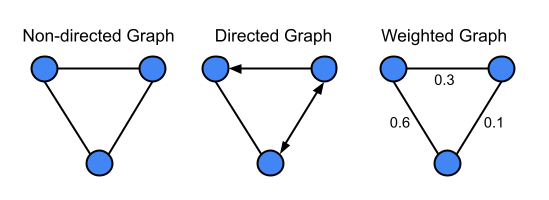
\includegraphics[width=0.85\textwidth]{images/3-track-reconstruction/Graphs.png}
  \caption{
    Illustration of different graph types. Non-directed graphs contain edges with no direction. Directed graphs can contain edges with unidirectional or bidirectional edges. Weighted graphs associate a weight to each edge, the example above has normalised edge weights. All three graphs are fully connected, whereby a unique edge connects each pair of nodes.
  }
  \label{fig:graph-architecture-example}
\end{figure}


\subsubsection{Message Passing Paradigm}

Message passing is an important property in the design of graph networks. It allows the propagation of node features by exchanging information between adjacent nodes. The edges between nodes act as conduits, allowing the transfer of information in a given direction if the connection is active. Typically, this scheme is iterative in nature. It begins with an initialization of a state at each node in the network, where a state typically comprises node or edge features. The node $v$ then aggregates states from adjacent nodes in its local neighbourhood. Node representations are then updated based on an aggregation function, improving the precision of states local to each node. This process is then repeated with further message passing and neighbourhood information aggregation, allowing local information to spread globally throughout the network. GNNs can fully exploit the connectivity of their structure, and as a result the mechanism allows models to become sophisticated in learning both local and global behaviour. With the correct application, this type of framework has proved to be highly effective in ML.


%--------------------------------------------------
%	Chapter 3: Track reconstruction on graph networks
%---------------------------------------------------
\subsection{Track Reconstruction on Graph Networks}
\label{track-recon-graph-networks}

In this thesis a novel methodology is investigated exploring the use of a GNN architecture as a solution to the track pattern recognition problem. There are two main aspects to this approach; a procedure to construct a graph network is presented in Chapter \ref{chapter-4} and a method to refine its connections and extract tracks is presented in Chapter \ref{chapter-5}. 

In order to identify compatible connections, a ML-based algorithm is used to predict the graph adjacency matrix, given input hit features such as the charge distribution in the cluster. An iterative procedure allows ambiguities in the network to be identified and tracks to be isolated. To efficiently exploit a priori knowledge about charged particle dynamics the GNN-based algorithm uses simplified KFs as mechanisms for information propagation as well as for track extraction. 

% In order to build the graph network, a ML-based algorithm will be used to predict the graph adjacency matrix, given the input hit features such as shape of a charge cluster representing a track position measurement in a silicon detector.

%Traditional MLP Training - ExaTrkX and others
% considering previous approaches and new ideas that stemmed from TrackML --> this led to my research
% Then move onto my research and approach

%Novel Deep Learning Methods for track reconstruction
%- Use GNNs for hit classification and segment classification
%- MLP implementation, deep network, many hidden layers
%- Purity 99.5%, Efficiency 98.7%
%- arXiv: 1810.0611, Hep.TrkX Project

%Accelerated Charged Particle Tracking with Graph Neural Networks on FPGAs
%- arXiv:2012.01563
%Graph Neural Networks for Particle Tracking (https://exatrkx.github.io)
% https://arxiv.org/pdf/2203.12852.pdf  - reconstruction section
%--------------------------------------
%	Chapter 4. ML Hit-Pair Predictor
%--------------------------------------


\doublespacing
\newpage
%\setcounter{section}{3}
%\section{The Compressed Pattern Space}
\chapter{Machine Learning Hit-Pair Predictor} 
\label{chapter-4}

When constructing graph networks for track reconstruction, one must first consider the ability to identify compatible edge connections to build track seeds. A beneficial step towards enhancing this process is to reduce the number of fake seeds constructed and hence increase the accuracy in predicting such compatible hit-pairs. As future upgrades to particle detectors will be problematic for the silicon tracking detectors where hit occupancy is the largest, it is essential that resource use is also reduced, whilst maintaining the capability to reconstruct tracks with minimal efficiency loss. This chapter presents a methodology to accomplish such a task. This work is presented in the Journal of Physics: Conference Series \cite{Lad_2023} and is implemented in the optimisation of the HLT ID track seeding software for ATLAS Run-3 and beyond \cite{Grandi:2728111, Long:2813981}. Section \ref{measurement-to-track-association} presents the development of an ML-based algorithm to predict if a pair of hits belong to the same track given input hit features, focusing on cluster width and inverse track inclination. The implementation of the trained predictor in the form of Look-Up Tables is presented in Section \ref{application-of-hit-pair-predictor}, alongside performance results including tracking efficiency and speed-up factor using simulated data is also discussed.


\section{Measurement to track association}
\label{measurement-to-track-association}

\subsection{Data Exploration and Feature Extraction}

%  TIP: Top quark simulation is often used for algorithm validation due of many possible final states including electron muon and $\tau$ lepton, \textit{b, c} and up quark. The decay signature of a top quark is complex as there are many of them, such that the combinatorics of the resulting seeds formed are high. - This makes top quark simulated events useful here

- also write about fake seeds here
  - pixel only seeds, reducing the fake rate. 
% mention the importance of why pixel based ML-based classifier is needed, the hit occupancy etc - most advantageous and beneficial here.
%The training is focused on pixel-detector layers, being closest to the beamline and thereby an advantageous region to reduce the proportion of fakes. The classifier predictions are used as input in the Fast Tracking algorithm.

Seeds constructed at the combinatorial stage of ATLAS track seeding from the Run-2 geometry were used to extract hit-pairs to form a training dataset. Monte Carlo (MC) $t\bar{t}$ samples with centre-of-mass energy $\sqrt{s}$ = 13 TeV at mean pile-up interaction multiplicity $< \mu >$ = 80 were used. An illustration of a seed in the ID pixel layers is shown in Figure \ref{fig:triplet-illustration}. From each triplet seed, the inner doublet (defined as hit-pair 1 and 2) and outer doublet (defined as hit-pair 2 and 3) are extracted. For each doublet the minimum and maximum absolute inverse slope of the track, $|cot(\theta)|$, were calculated using $r$-$z$ coordinates and used as an input feature for training. $\theta$ is the angle of inclination of a hit-pair with respect to the $z$ axis. The longitudinal pixel cluster width, $w_{\eta}$, measured in the $\eta$ direction was also extracted, where $\eta$ is defined in Eq. \ref{eq:pseudorap}. The MC generated data in the [$|cot(\theta)|$, $w_{\eta}$ ] phase space behaves as a set of 1-dimensional distributions, each with discrete $w_{\eta}$. This characteristic is exploited to form an ensemble of predictors. MC truth for seeds and their corresponding doublets were extracted from ATLAS track seeding and used as targets in training. Doublets with correct hit association were defined as truth 1, for which its hit-pairs belong to the same track. Conversely doublets with incorrect hit association defined as truth 0, for which its hit-pairs do not belong to the same track. Hit-pairs for the pixel barrel and endcap are handled separately in order to build regional classifiers, where a similar methodology was used for both outlined in Section ...


\begin{figure}[!htbp]
\centering
    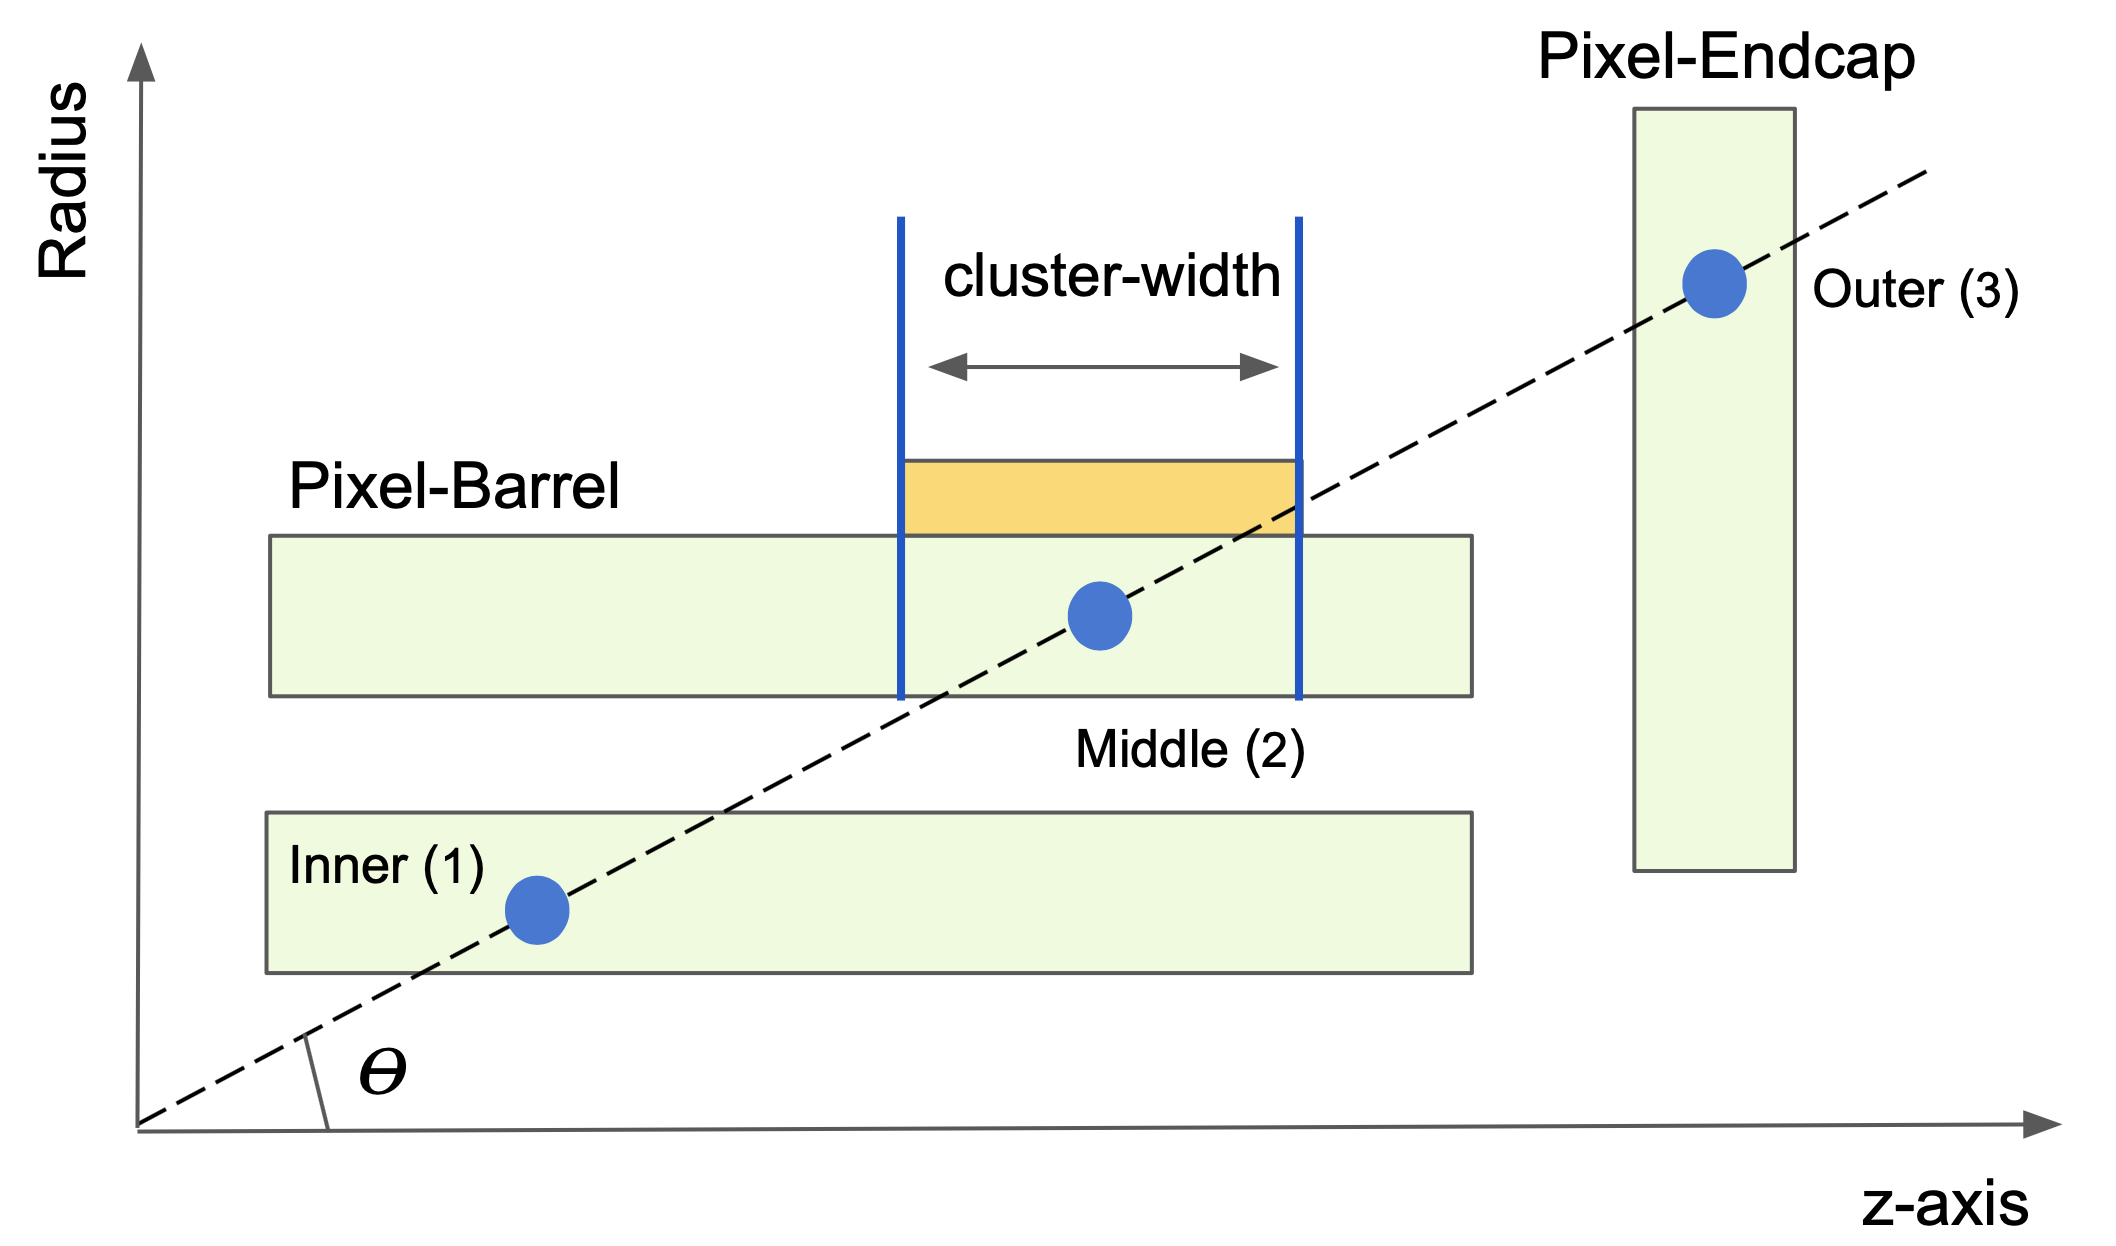
\includegraphics[width=0.8\linewidth]{images/4-ml-based-predictor/triplet_illustation.png}
    \caption{Seed illustration in the $r$-$z$ plane (mm) of the ID. The inner doublet consists of hits (1, 2) and the outer doublet consists of hits (2, 3). The longitudinal pixel-cluster width $w_{\eta}$ (mm) is measured in the direction of $\eta$, where $\theta$ is the angle of inclination with respect to the $z$ axis.}
\label{fig:triplet-illustration}
\end{figure}


\subsection{Classifier Development}

\subsubsection{Not-so-Naive Bayes}

The basis of Bayes’ theorem \cite{naive-bayes} is used to build a classifier to discriminate between doublet classes, for both the barrel and endcap regions. Bayesian analysis is based on having a prior probability of belief of an outcome of an event and a likelihood probability, where naive Bayes’ assumes that the conditional probabilities of the independent variables are statistically independent. The final classification is produced by computing the posterior probability by combining both the prior beliefs and the likelihood, which then determines the most probable class label. Using Bayes’ theorem is advantageous in this data-driven setting, as prior knowledge of the behaviour of the system is known. The posterior probability $P(c|x)$ that a given data point x belongs to class c is defined as:

\begin{equation} \label{naive-bayes}
    P(c|x) = \frac{P(x|c)P(c)}{P(x)}
\end{equation}

$P(x|c)$ is the conditional likelihood, $P(c)$ is the class prior probability and $P(x)$ is the predictor prior probability, used for normalisation and calculated from the number of data points belonging to class $c$.

Bayes' theorem is implemented using a generative model for each class. This was achieved by computing the likelihood function via a Kernel Density Estimate (KDE) for each of the 1-dimensional $\tau$ distributions, forming a set of generative Bayesian classifiers. This method removes the 'naive' element and performs the same classification with a more sophisticated generative model for each class.

\subsubsection{Kernel Density Estimation}

KDE is a non-parametric approach to estimate the probability density function of a random variable. The idea is that a kernel function is defined and centred on each data point in the sample. The sum of these functions together forms the kernel density estimate. The kernel density is defined as:
    
\begin{equation} \label{eq2}
    \hat{f}(x) = \frac{1}{Nh}  \sum_{i=1}^{N} K \left( \frac{x - x_i}{h} \right)
\end{equation}

where $K(x)$ is the kernel function, typically a smooth, symmetric and non-negative function, $h > 0$ is the smoothing bandwidth that controls the amount of smoothing applied to the function and N is the number of sample points used for normalisation \cite{kde}. The KDE must be normalised in order to represent a probability density. For this study the Gaussian kernel function is implemented to approximate the probability density at each data point in the sample. One advantage of using KDE is that it provides a more flexible estimator parameterised by $h$. The Gaussian kernel is defined as:
    
\begin{equation} \label{eq3}
    K(x) = \frac{1}{\sqrt{2\pi}} e^{\frac{-x^2}{2}}
\end{equation}

The choice of bandwidth is important, as increasing the bandwidth too high results in a smooth distribution where granular information is lost (over-smoothing). When using a bandwidth that is too small, this can lead to narrow peaks in close proximity to each other, resulting in a very noisy distribution (under-smoothing). There are several methods to determine the optimum bandwidth discussed in \cite{bandwidth-selection-methods}, many of which show similar properties. The method used in this study was the so-called \textit{Silverman's rule of thumb}, which works only for 1-dimensional data. Silverman's rule finds the bandwidth that minimizes the mean integrated squared error assuming that the data is Gaussian and a Gaussian kernel was used.

\subsection{Classifier Training}

%Figure \ref{fig:1-dimensional-classifier-training} shows distributions of $\rvert cot(\theta)\rvert$ for Pixel barrel hit pairs in the ATLAS pixel detector, where $\theta$ is the inclination angle of the doublet with respect to the $z$-axis. from t ̄t Monte Carlo 13 TeV with mean pile-up interaction multiplicity of <μ> = 80. Shown are pixel-barrel doublets from triplets constructed at the combinatorial stage in ATLAS track seeding. These triplets are formed from pairs of doublets which share a common spacepoint where that shared middle spacepoint consists of pixel clusters with wη ≤ 0.4 mm, where wη is the cluster width measured in the η direction. Shown are the distributions for doublets with hits correctly associated to corresponding truth particles by the tracking algorithms, for which its doublet spacepoints belong to the same track and also shown are doublets that have hits incorrectly associated, for which its spacepoints do not belong to the same track. The data was used to train a Machine Learning classifier to predict whether a doublet of spacepoints has correct hit association and hence belong to the same track corresponding to truth particles, or incorrect hit association, using the input hit features of wη and the absolute inverse track inclination |cot(θ)|. This study was conducted in order to speed up the track seeding stage and reduce CPU time in the ATLAS fast tracking trigger algorithm.

% roc curve:
%Shown is the Receiver Operating Characteristic (ROC) curve indicating the rates of false positive and true positive of pixel-barrel doublets from the ATLAS pixel detector to tracks corresponding to truth particles, for spacepoints with wη ≤ 0.4 mm, where wη is the cluster width measured in the η direction, using a Machine Learning (ML) classifier to predict whether a doublet of spacepoints belong to the same track and hence defined as having correct hit association, or have incorrect hit association. The classifier was trained using pixel-barrel doublets from Monte Carlo 13 TeV t ̄t <μ> = 80 samples. Each pair of false positive and true positive rates correspond to a prediction probability, which can be used as a tuning parameter. The classifier’s predictions were adjusted using the prediction probability derived from the ROC curve which would yield a true positive rate of 0.95. The Area Under the Curve (AUC) is a measure of the ability of the classifier to distinguish between correct and incorrect hit association classes and is in the range 0.0 ≤ AUC ≤ 1.0, where AUC = 1 corresponds to perfect classification. The AUC achieved by the ML classifier shown was AUC = 0.79. Also shown is the ‘no skill’ classifier result with AUC = 0.5, which cannot discriminate between correct or incorrect hit association classes and would predict a random class in all cases with 50% probability for each class. A similar procedure was executed for training a model to determine whether spacepoints in pixel-endcap doublets belonged to the same track, using truth from Monte Carlo 13 TeV t ̄t <μ> = 80 samples. This study was conducted in order to speed up the track seeding stage and reduce CPU time in the ATLAS fast tracking trigger algorithm.

\begin{figure}[!htbp]
\centering
    \begin{subfigure}[a]{0.9\textwidth}
        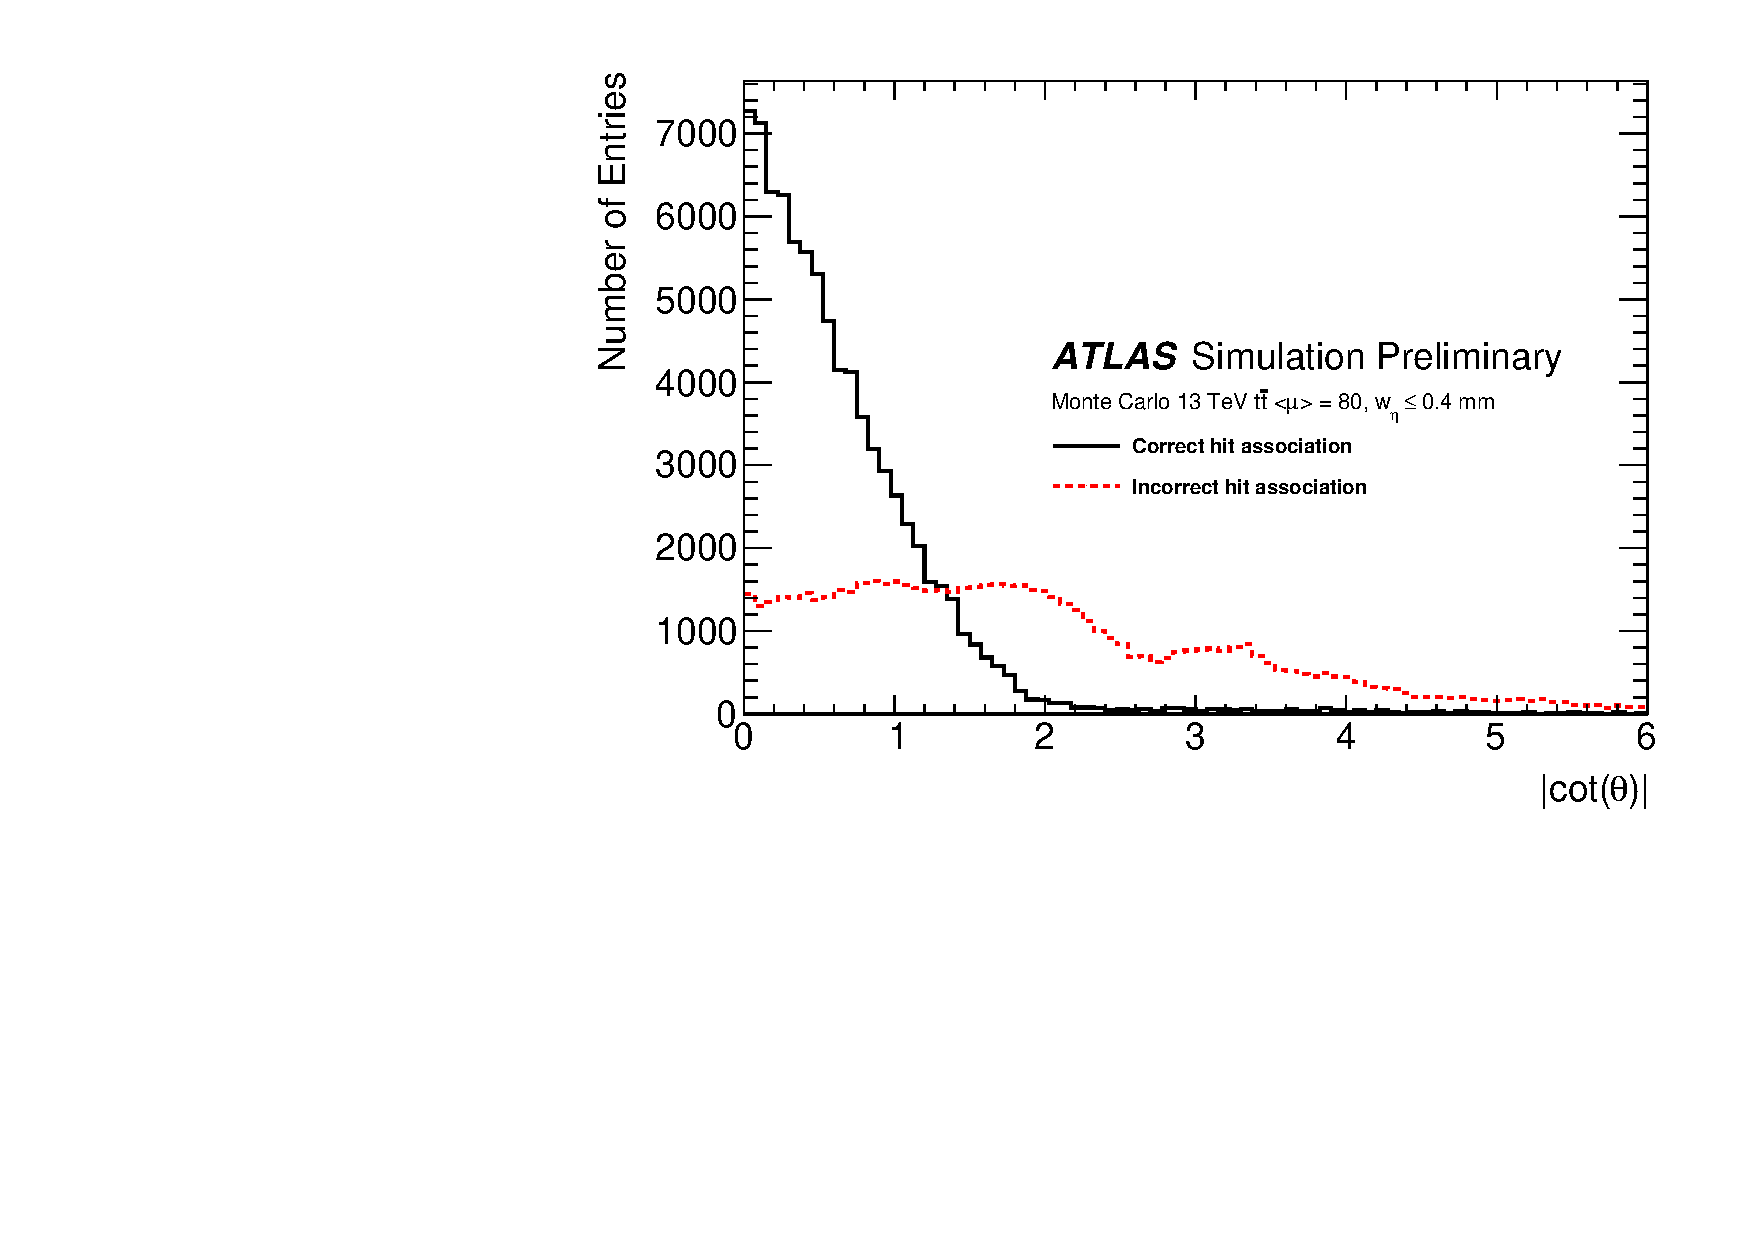
\includegraphics[width=\linewidth]{images/4-ml-based-predictor/histo.pdf}
        \caption{$\lvert cot(\theta) \rvert$ distributions for Pixel barrel hit pairs with $w_{\eta} \leq 0.4$ mm }
        \label{fig:truth-histo}
    \end{subfigure}
    \hfill
    \begin{subfigure}[b]{0.9\textwidth}
        \centering
        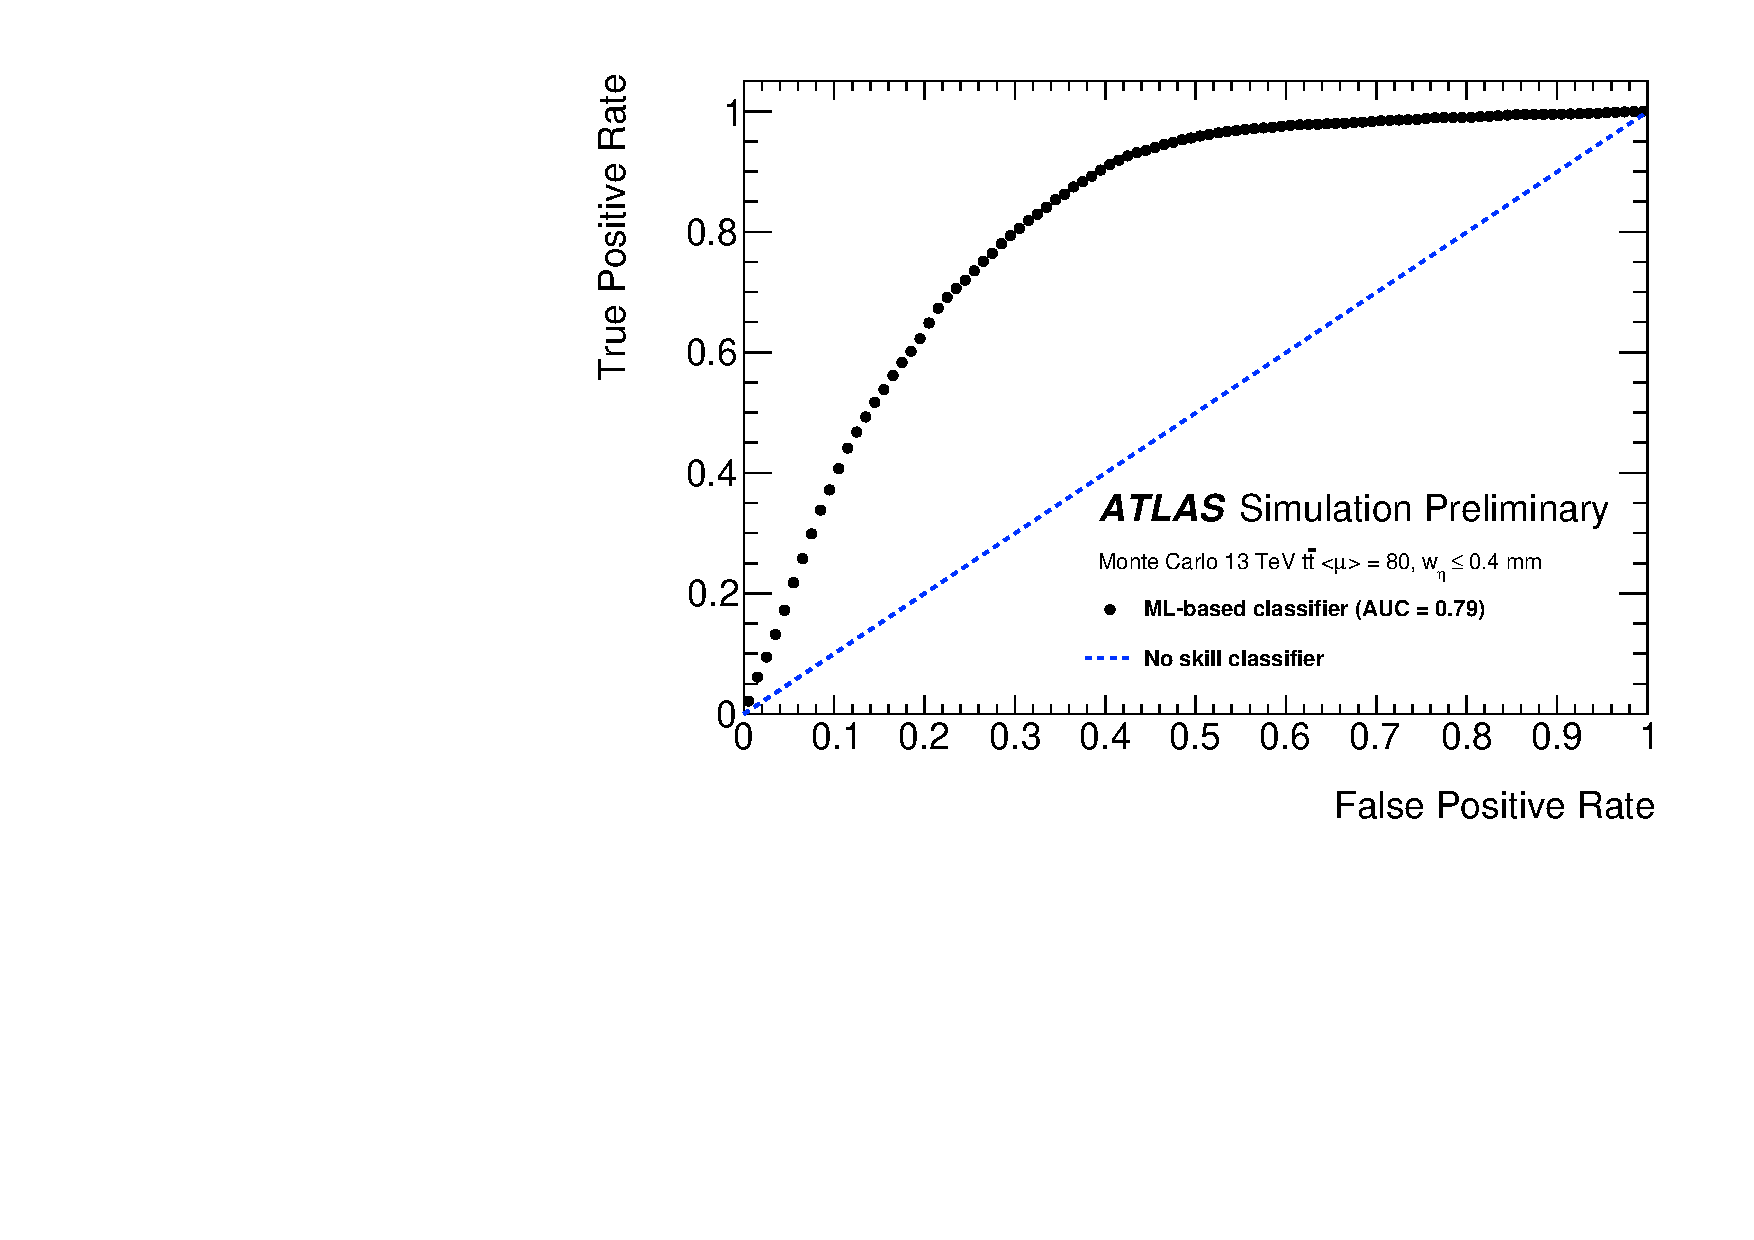
\includegraphics[width=\linewidth]{images/4-ml-based-predictor/roc.pdf}
        \caption{ROC curve for Pixel barrel hit pairs with $w_{\eta} \leq 0.4$ mm }
        \label{fig:roc-curve}
    \end{subfigure}
\caption{(a) $\lvert cot(\theta) \rvert$ for Pixel barrel hit pairs in the ATLAS Pixel detector, where $\theta$ is the inclination angle of the hit pair with respect to the $z$-axis. (b) The corresponding Receiver Operating Characteristic (ROC) curve for the classifier trained on the data shown in (a). The curve indicates the rates of false positive and true positive of Pixel barrel hit pairs to tracks corresponding to truth particles.}
\label{fig:1-dimensional-classifier-training}
\end{figure}


\subsection{Probability Calibration}

\subsection{Classifier Predictions and Evaluation}


\begin{figure}[!htbp]
\centering
    \begin{subfigure}[a]{0.86\textwidth}
        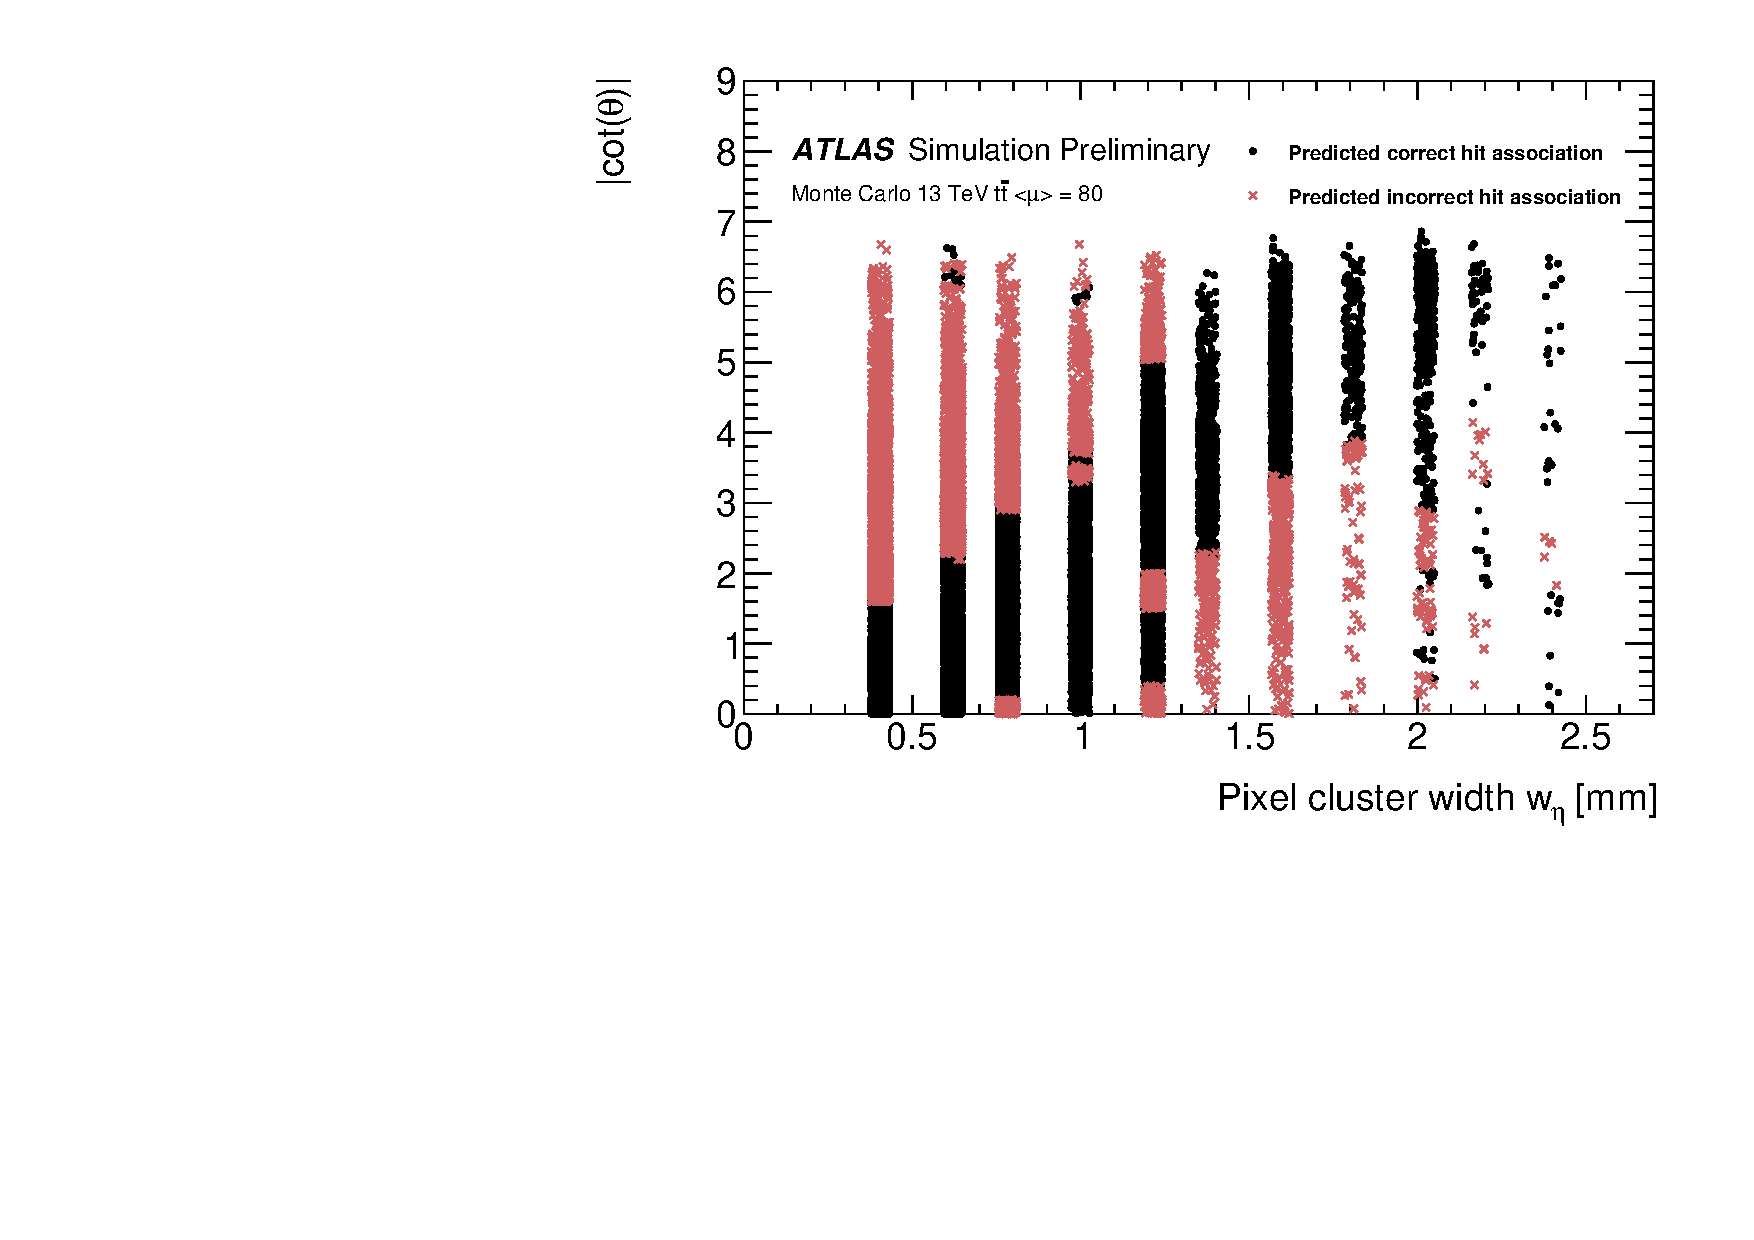
\includegraphics[width=\linewidth]{images/4-ml-based-predictor/scatter_kde_predictions.pdf}
        \caption{XXXX}
    \end{subfigure}
    \hfill
    \begin{subfigure}[b]{0.86\textwidth}
        \centering
        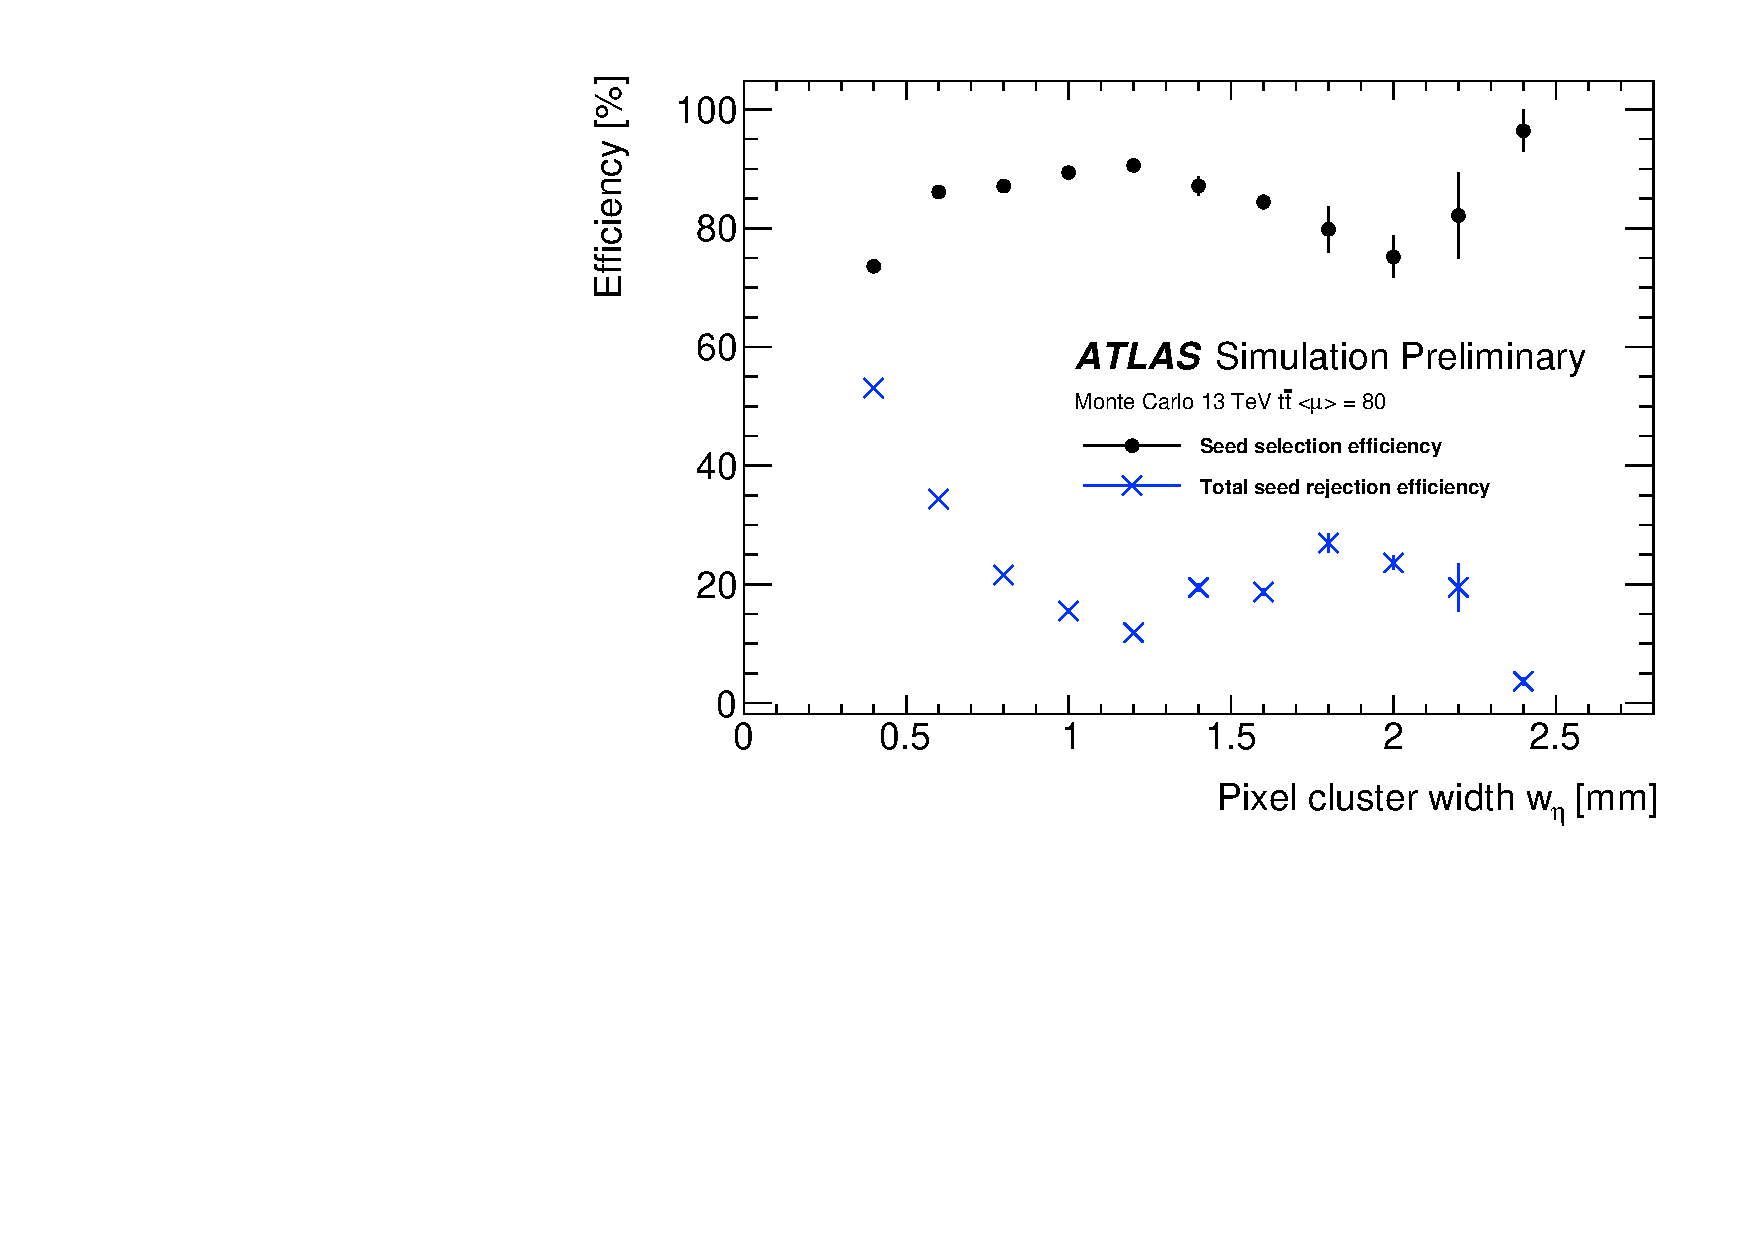
\includegraphics[width=\linewidth]{images/4-ml-based-predictor/triplet_eff_metrics.pdf}
        \caption{XXXX}
    \end{subfigure}
\caption{XXXX}
\label{fig:predictions-pixel-barrel-and-triplet-efficiencies}
\end{figure}


\section{Application of hit-pair predictor}
\label{application-of-hit-pair-predictor}

\subsection{Look-Up Table Generation}

Classifier predictions are converted into Look-Up Tables (LUT) such that the acceptance region can be fed into the FTF. Using a predefined LUT is a much more efficient procedure than computing class label on the fly and it is very low cost to store in memory. It consists of binning both the W eta axes (45 bins between 0.0 - 3.0) and the $\tau$ axes (30 bins between 0.0 - 3.0), recording the bin numbers to accept. These divisions were chosen such to compare with the current estimation, referred to as strict LUT.

\subsubsection{Morphological Filtering}

An ensemble approach was taken combining the strict LUT and KDE predictions. Morphological filtering was then applied to achieve a smoothed structure. Morphological filtering is an image processing technique whereby non-linear transformations are applied to the binary matrix of an image, altering the features. Such non-linear operations include dilation and erosion. Dilation enlarges bright regions and shrinks dark regions, whereas erosion does the inverse of this. A combination of dilation and erosion was applied to the ensemble LUT via rectangular structuring elements, in order to encourage horizontal
extrapolation of the acceptance region. The binned predictions from the KDE classifiers and smoothed LUTs are shown in Figures 9 and 10; orange representing acceptance regions and blue rejection regions.
Referring to 9a, KDE predictions for the barrel coincide well with the ’linear corridor’ estimation from the strict LUT. Whereas a V-shaped LUT is obtained for the endcap region.


\subsection{ML filtering modes}

\subsection{Seed Classes}



\subsection{Performance Evaluation}

There is little deviation from the standard trigger seeding with application of the machine learning extensions, where the average tracking efficiency achieved was 93.9\% and the greatest efficiency loss from the standard trigger seeding is at large $\lvert \eta \rvert$.

\begin{figure}[!htbp]
\centering
    \begin{subfigure}[a]{0.86\textwidth}
        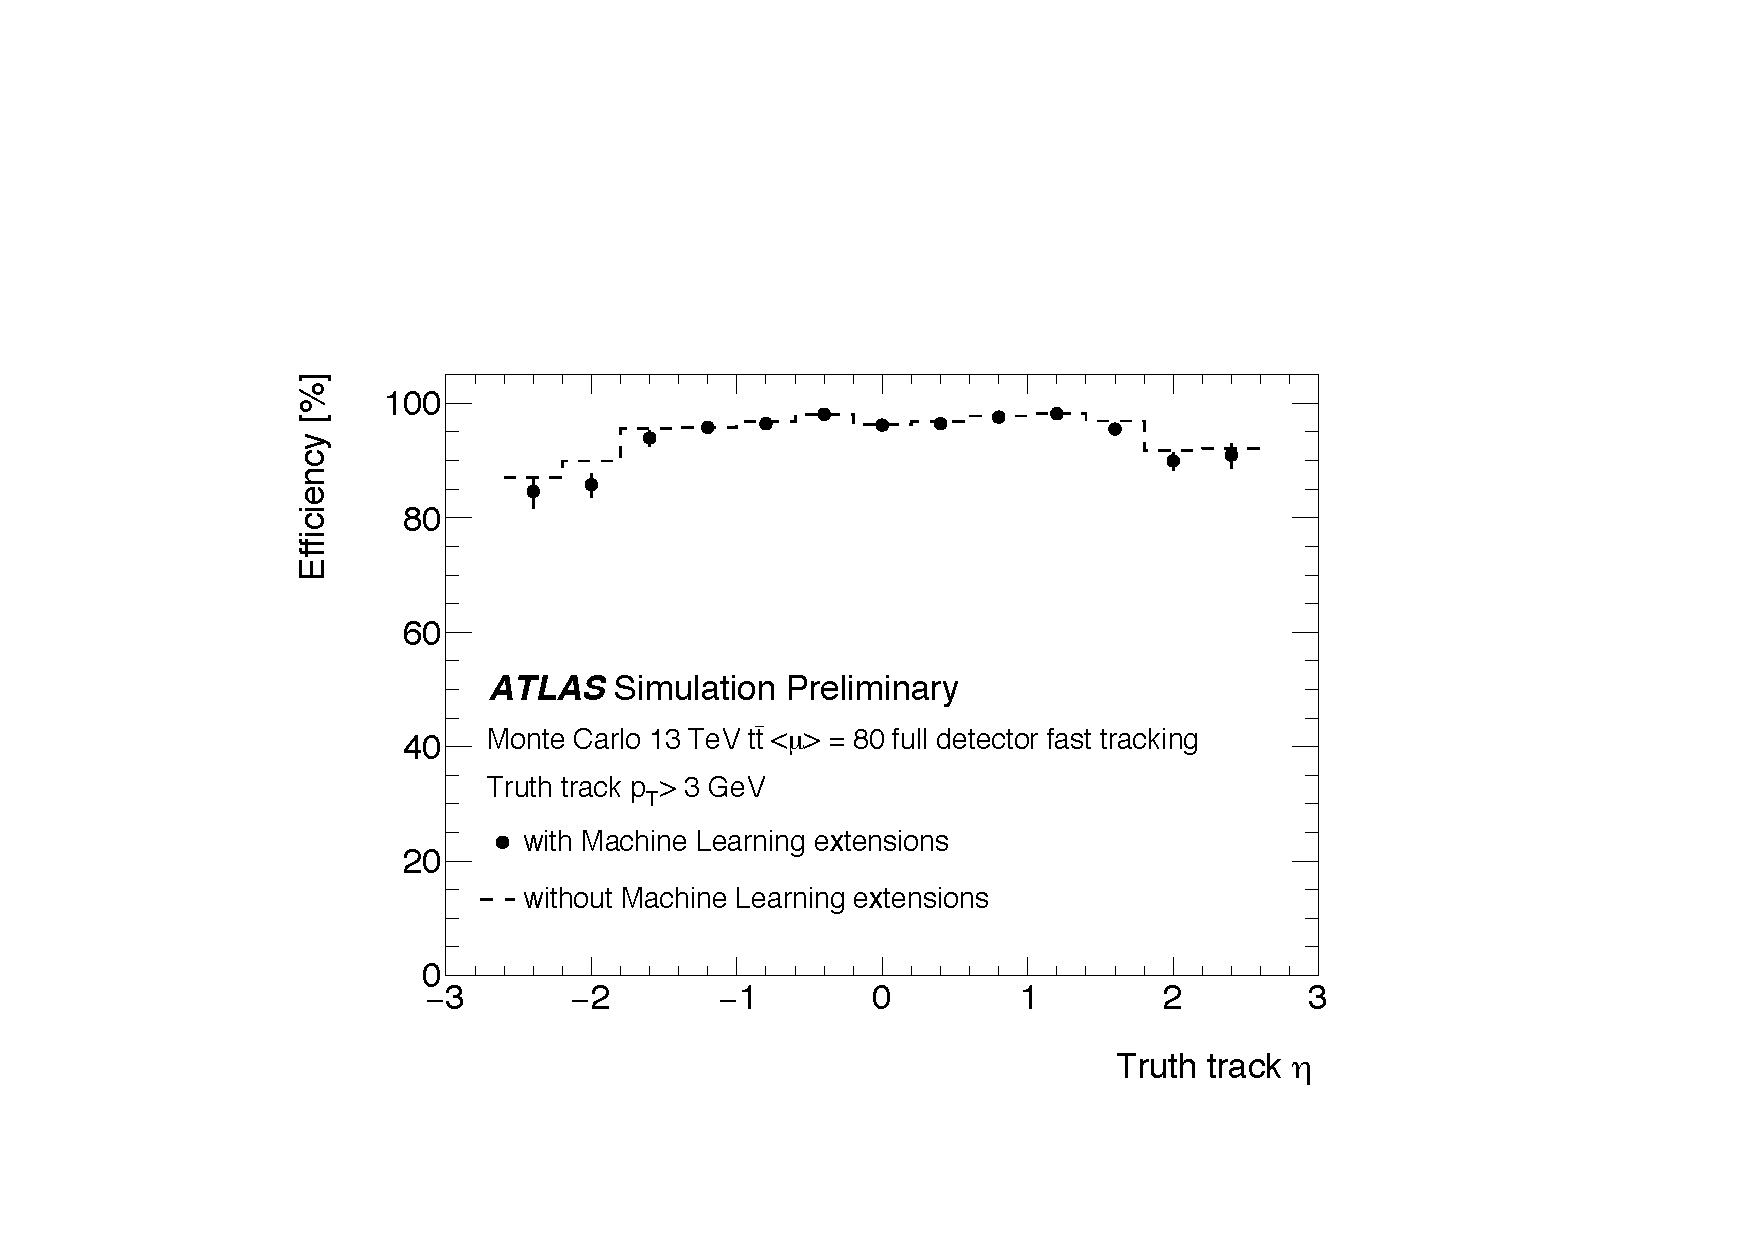
\includegraphics[width=\linewidth]{images/4-ml-based-predictor/efficiency_eta.pdf}
        \caption{Efficiency vs. MC truth track $\eta$}
    \end{subfigure}
    \hfill
    \begin{subfigure}[b]{0.86\textwidth}
        \centering
        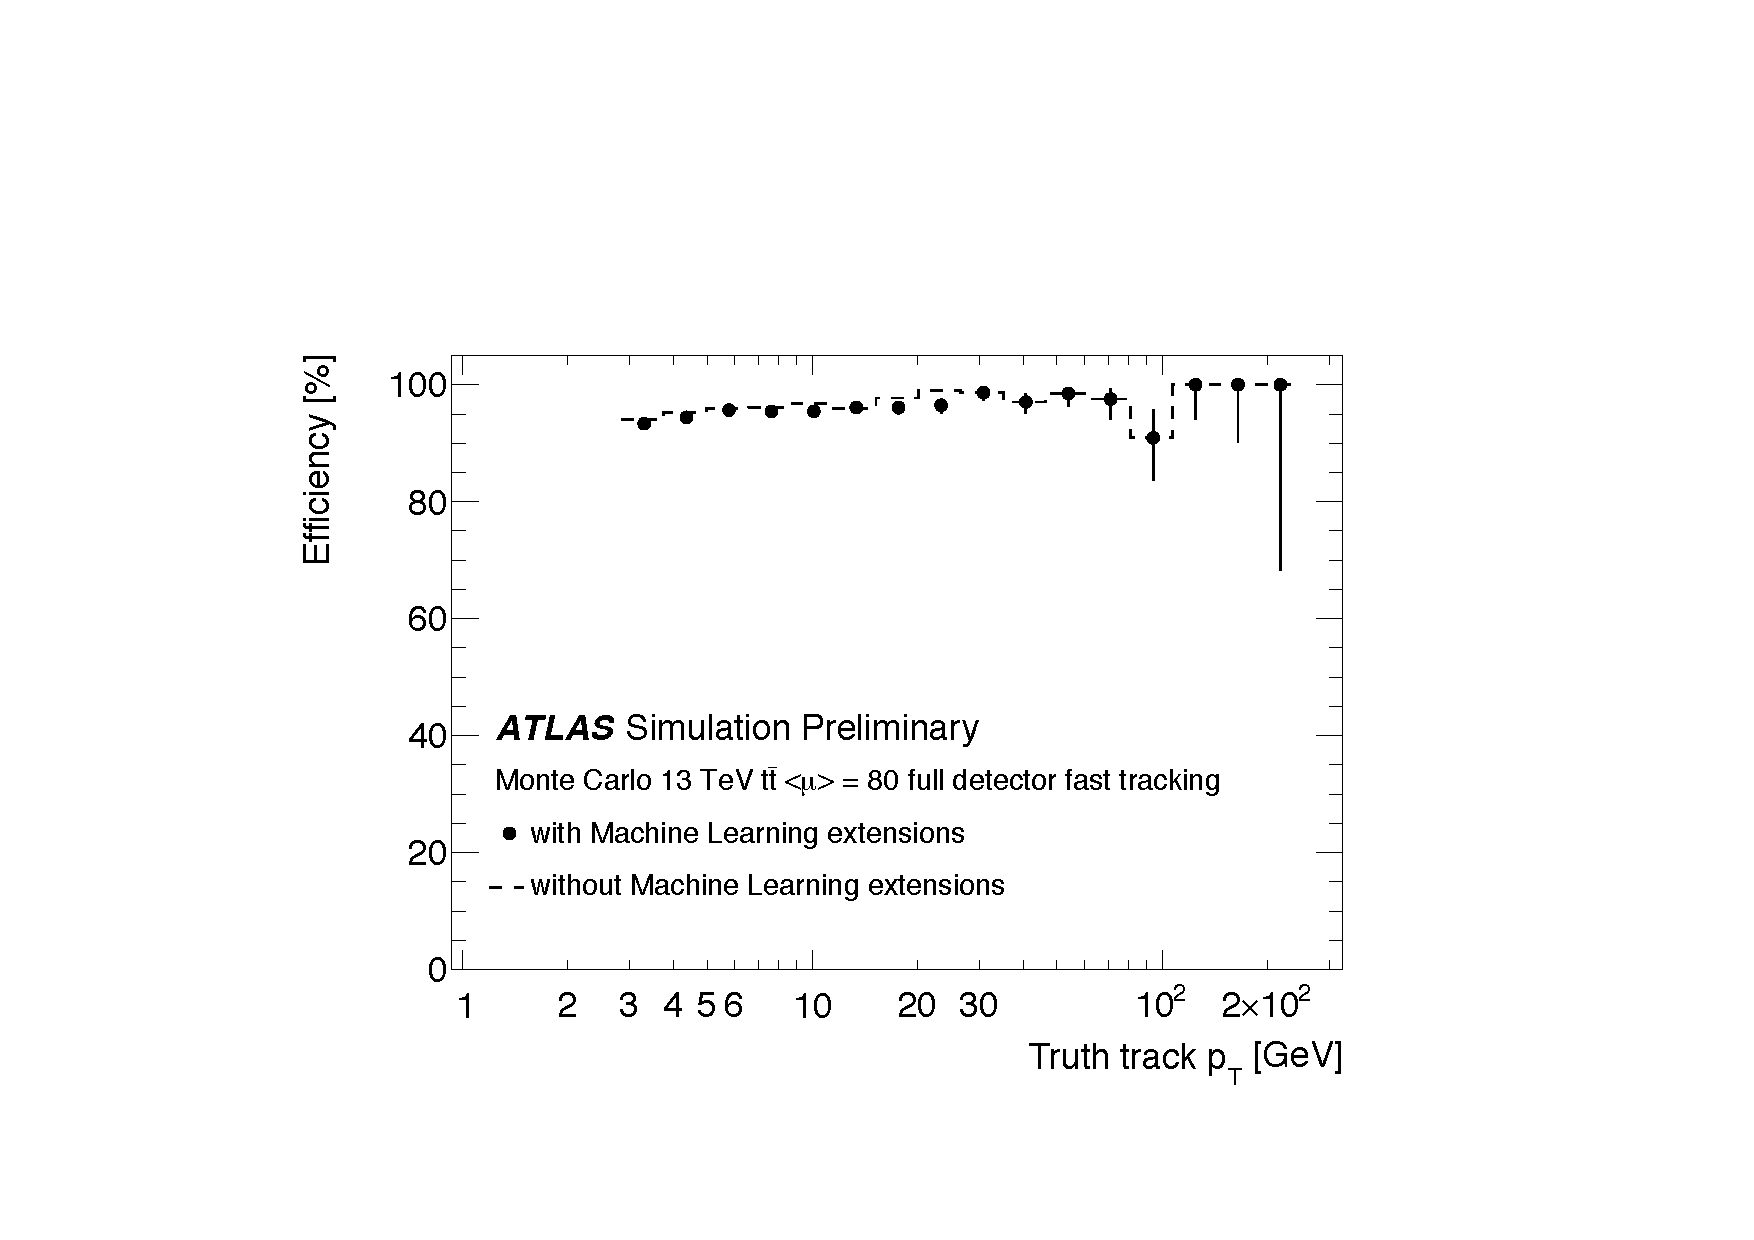
\includegraphics[width=\linewidth]{images/4-ml-based-predictor/efficiency_pT.pdf}
        \caption{Efficiency vs. MC truth track $p_{\mathrm{T}}$}
    \end{subfigure}
\caption{Tracking efficiencies as a function of track parameters, for $p_{T}$ > 3 GeV for the ATLAS full detector tracking with $t\overline{t}$ Monte Carlo 13 TeV and mean pile-up interaction multiplicity of $\langle \mu \rangle$ = 80. The data points show the efficiency when using machine learning extensions in the seed building stages of the fast tracking trigger in the ATLAS pixel detector, prior to the track fitting. The dashed line shows the efficiency of the standard trigger seeding with no application of machine learning extensions. The errors shown are purely statistical \cite{public-hlt}. }
\label{fig:efficiencies-ml-hit-pair-predictor}
\end{figure}



\subsubsection{CPU Time Comparison}

Table \ref{tab:cpu} summarises the breakdown in speed-up factor achieved at various stages within the \texttt{Fast Tracking} trigger algorithm, with the application of the trained LUT for the pixel region. The greatest saving in CPU time is achieved during the \texttt{Seed Processing} stage, as a direct result of a significant reduction in the number of seeds. The average number of seeds processed for a given region of interest for the standard tracking is $O(10^{4})$, whereas with the introduction of ML filtering for pixel seeds, about 78\% fewer seeds were observed. This significant reduction in CPU time does not only benefit the \texttt{Seed Processing} stage of the combinatoric track following, but also propagates to \texttt{Track Fitting}.

\begin{table}[htb!]
\caption{Performance of the ATLAS full detector tracking with MC 13 TeV $t\bar{t}$ samples at $<\mu> = 80$, with the application of ML extensions for filtering on pixel detector hit-pairs in the \texttt{Fast Tracking} trigger stage \cite{public-hlt}. The total speed-up factor and breakdown of speed-ups at different stages of the \texttt{Fast Tracking} trigger algorithm are presented, each speed-up is presented with respect to the standard trigger seeding where no ML extensions were applied.}
\begin{center}
\begin{tabular}{llll}
\toprule
Total Speed-up Factor & Seed Generation & Seed Processing & Track Fitting \\
\hline
2.3 & 1.3 & 3.3 & 1.5 \\ 
\bottomrule
\end{tabular}
\end{center}
\label{tab:cpu}
\end{table}

\subsubsection{Changing Pileup Conditions}
Table \ref{tab:pileup} summarises the relative efficiency loss and relative speed-up factor, with application of ML extensions for the ATLAS pixel detector in various mean pile-up interaction multiplicities $<\mu>$. The speed-up factor increases as $<\mu>$ increases with minimal loss in efficiency.

\begin{table}[htb!]
\caption{Performance of the ATLAS full detector tracking with MC 13 TeV $t\bar{t}$ samples at $<\mu>$ = 40, 60 and 80, with the application of ML extensions for filtering on pixel detector hit-pairs in the \texttt{Fast Tracking} trigger stage prior to the track fitting \cite{public-hlt}. The absolute loss in average tracking efficiency and the total speed-up factor for seeded track finding in the ATLAS pixel detector are presented with respect to the standard trigger seeding where no ML extensions were applied. The efficiency loss is mainly observed at large $|\eta|$. The statistical uncertainties in efficiencies are $O(10^{-3})$, hence are not quoted.}
\begin{center}
\begin{tabular}{ccc}
\toprule
$<\mu>$ & Efficiency Loss (\%) & Total Speed-up Factor  \\
\hline
40 & 0.7 & 1.6 \\
60 & 0.7 & 2.1 \\
80 & 1.1 & 2.3 \\
\bottomrule
\end{tabular}
\end{center}
\label{tab:pileup}
\end{table}


\section{Other Approaches}
\subsection{Multiple Acceptance Regions}

When training With varying permutations of train and test sets, a second acceptance region was frequently predicted for the barrel at low-cluster width and high track inclination angle, highlighted in Figure \ref{fig: multiple-acceptance}. The spacepoints predicted as belonging to the $good$ doublet class at the tail ends of these distributions were isolated and their local cluster position in the $\eta$ direction were considered, see Figure \ref{fig: multiple-acceptance}. The majority of hits possessed the largest absolute local cluster position. This was observed for each occurrence of a second acceptance region appearing at low cluster-width and high track inclination. This corresponds to the extremes of the barrel module, since its dimensions are approximately $20mm$ $x$ $60mm$ \cite{pixel-module-dimensions}, and hence the second acceptance region had originated from module edge pixels. These spacepoints would need to be dealt with separately or accepted by default. One reason for this is, due to the fact that the morphological smoothing is applied uniformly to an image, this will affect the shape of the main acceptance region for the barrel and will introduce a greater proportion of fakes by dilation.
    

\subsection{Support Vector Machine}

% See this website for further explanation 
% https://towardsdatascience.com/support-vector-machine-introduction-to-machine-learning-algorithms-934a444fca47

% multi class classification: one-to-rest
% https://towardsdatascience.com/multiclass-classification-with-support-vector-machines-svm-kernel-trick-kernel-functions-f9d5377d6f02

Another supervised learning algorithm investigated was the Support Vector Machine (SVM) \cite{svm}. The objective of the SVM classifier is to find a hyperplane (known as a decision boundary) in a N-dimensional space (where N is the number of features) that distinctly classifies the data points and is typically used in binary classification. The optimal decision boundary is one which maximizes the margins between both classes, this provides some reinforcement that future data points can be classified with more confidence. For non-linear decision boundaries, the SVM uses the so-called \textit{kernel trick} to project the data into a higher dimensional space. 

% what the SVM was applied on - the plane of axes. SVM would be normally applied to the plaine of ... however we need to transform it using PCA bec of ... So we end up principal component axes, the 1st axes shows, the 2nd shows...


A prior step to training the SVM classifier, was to apply Principal Component Analysis (PCA).

A combination of Principal Component Analysis (PCA) and SVM was applied. PCA is commonly used as a dimensionality reduction technique \cite{pca}, however in this instance it is applied to remove the ordinal nature (the discrete bands) which affects the SVM and hence obtain a continuous 2D-dimensional phase space. 

% further detail on training the SVM

A hyper-parameter sweep of various kernels was executed using cross-validation and the polynomial kernel of third degree was found to produce the highest TPR. The predictions of the PCA-SVM classifier on Pixel barrel data is shown in Figure \ref{fig:barrel-svm-pca}. The red (orange) region shows which doublets are accepted and the blue region shows which doublets are rejected. The corresponding data points also reflect class predictions. 

SVMs generally perform well, even when trained with imbalanced data sets. This coupled with the fact that a distinct decision boundary could be easily extracted and converted into a LUT would lead to less ambiguity in comparison to applying an extrapolation using morphological smoothing. However, there are key disadvantages by using a SVM classifier rather than Bayes' theorem in this instance. The probabilistic information contained within each discrete 1 dimensional distribution of $w_{\eta}$ is lost, which is an important feature when tuning each individual distribution. Additionally, the SVM typically fits a continuous function for the decision boundary and hence may not be strict enough in certain regions. This factor is important when considering the number of fake seeds being accepted using a LUT generated from such a decision boundary. 


\begin{figure}[!htbp]
\centering
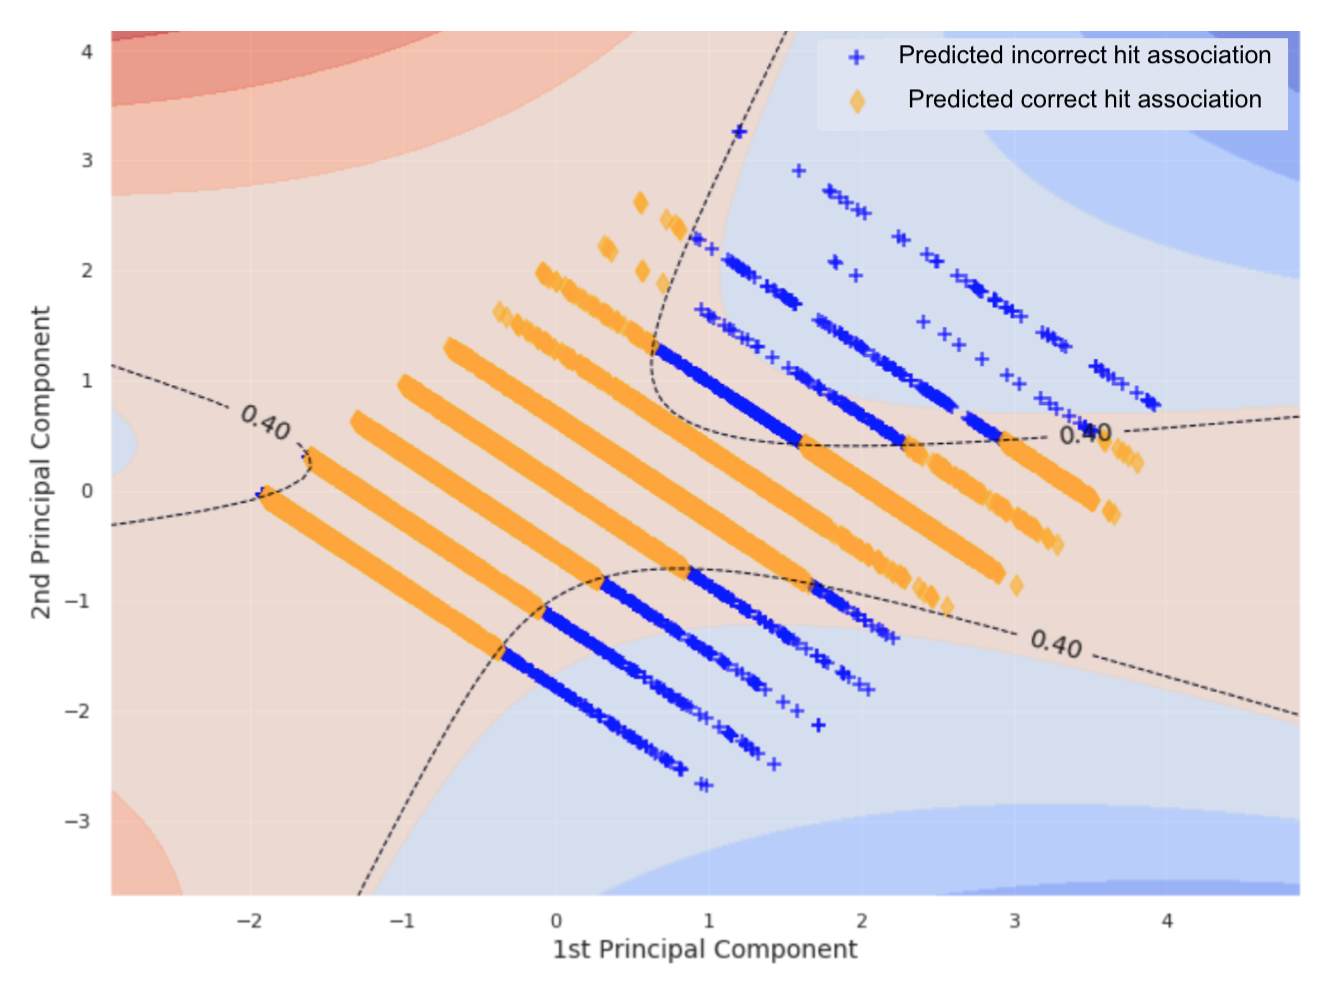
\includegraphics[width=0.85\linewidth]{images/4-ml-based-predictor/barrel-svm-pca.png}
\caption{PCA transform applied to the pixel barrel hit pairs. SVM classifier decision boundary predictions are shown in the above plot. The black dotted line represents the threshold value of 0.40, yielding a TPR of 95\%. The SVM kernel used for the classifier was a polynomial degree 3 kernel with hyperparameters $C=0.75$ and $\gamma=0.05$. 1st principal component indicates the axis of largest variance within the class with correct hit association doublet class.}
\label{fig:barrel-svm-pca}
\end{figure}

Figure \ref{fig:barrel-svm-pca} it is clear to see that the area of acceptance predicted by the SVM is much greater than the KDE based classifier. The seed multiplicity in these areas would inevitably lead to a larger amounts of time spent on processing seeds through the combinatorial stage of the FTF. Therefore this method was not pursued. However, a further investigation would be needed to evaluate the efficiency and speed-up provided from these predictions, compared with the KDE based classifier.


\subsection{Comparison with Deep Learning Algorithm}

Comparison with outrunner algorithm (number 2 in TrackML) - deep learning methodoloy vs. our classic ML approach.


\section{Conclusions}

% ---------------------------------------
% TODO
% ---------------------------------------
%At the end of this chapter, mention that a similar classifier was implemented to find pairs of hits for TrackML algorithm as well. Interestingly it also goes to a LUT input because this is the fastest way to do inference and implement this in any realistic detector setup, instead of training the classifier each time on the fly. Of course, for different geometrical setups or for particular signatures i.e. jets, the training would need to be done again specifically for that purpose.

As the luminosity, and hence collision rate, increases during future upgrades of the LHC program, novel and precise tracking methodologies, as well as efficient use of computing power will become an increasingly
important factor in the selection of physics objects.

The application of a ML-based classifier for seed selection in the ATLAS ID has provided significant CPU savings on trained MC data at various pileup levels. The trained predictor in the form of a LUT yields 2.3$\times$ speed-up with minimal loss in efficiency (1.1\%) at $< \mu >$= 80 compared with the standard trigger tracking. The developed ML pipeline provides a way to generate custom LUTs by training the predictor to yield a required TPR, dependent on the degree of efficiency required. Reducing the proportion of fakes at an earlier stage in the ATLAS HLT track seeding, ensures the reduction in CPU usage overall. Efficient use of computing power will become an increasingly important factor in the selection of physics objects as the luminosity and pileup increase during future upgrades of the LHC program.

%It is encouraging to see that the use of a ML based classifier for seed filtering in the ID, together with the proper selection of seed types, has provided significant CPU savings based on trained MC data. The application of the trained KDE based predictor in the form of a smoothed LUT for seed filtering within the barrel and endcap, as well as propagation of high purity seed types, yields greater than 2x speed up with minimal loss in efficiency, compared with the default. By applying an ensemble approach in LUT generation, this results in a much smaller drop in efficiency than using the strict LUT estimation alone. The use of different ML filtering modes applied to the triplets, can produce varying efficiencies (and speed up), where the three least redundant combinations are presented in this study. This procedure also shows greater efficiency across full range in η for the ID, compared with the strict LUT, which rejects a larger proportion of good seeds, particularly within the high seed multiplicity (low cluster width) range. Additionally, proper training and tuning of the classifier can yield a required TPR, therefore allowing the flexibility in strictness. By reducing the proportion of fakes an at earlier stage in the HLT track seeding, this ensures the reduction of bad seed propagation into later tracking stages and hence saving CPU.


%--------------------------------------------------
%	Chapter 5. GNN Pattern Recognition Algorithm
%--------------------------------------------------

\chapter{Graph Neural Network Pattern Recognition Algorithm}\label{chapter-5}

Once compatible hit-pairs from a particle collision event have been established, they are used to build a graph network. This chapter presents a novel pattern recognition algorithm to prune outlier connections in such a network in order to reconstruct tracks, by utilising GNN architectures. The application of the GNN is focused on the Pixel detector, with the aim that the approach will serve as a sophisticated track seeding technique for Pixel hits and form preliminary track candidates. If the GNN does not produce large proportions of fake tracks, such an approach could save significant computational resources. The ultimate aim is to develop a realistic algorithm for fast track reconstruction that can be deployed in future high-luminosity upgrades of particle detector experiments. This research was presented at the 2022 Connecting the Dots (CTD) conference at the University of Princeton USA and at the dedicated GNN Google DeepMind seminar at UCL in 2023. At the time of writing this work was under review for publication in the Springer Journal: Computing for Software and Big Science \cite{Lad_2023_gnn}. This chapter is organised as follows; sections \ref{gnn-algorithm-overview} to \ref{gnn-track-extration} present a breakdown of the GNN algorithm and Section \ref{gnn-application-toy-model} illustrates an application on a simple toy MC model.


\section{Algorithm Overview}
\label{gnn-algorithm-overview}

In the context of GNNs, individual hits or clusters of hits are modelled as graph nodes and track segments are modelled as graph edges. Once the graph network is constructed, each edge is modelled as a Gaussian state in order to approximate the local track state probability density. Therefore, each node is initialised with a Gaussian mixture of track states, local to its neighbourhood of connections.

We consider the GNN-based pattern recognition algorithm as an iterative mixture reduction problem, which allows the deactivation of incompatible connections (GNN edges termed as outliers). This enables the improvement of track parameter estimates and iterative extraction of track candidates. 

After initialisation, the network evolves iteratively, where an iteration is made up of three main stages illustrated in Figure \ref{fig:flowchart}. 

\begin{figure}[htbp]
    \centering
    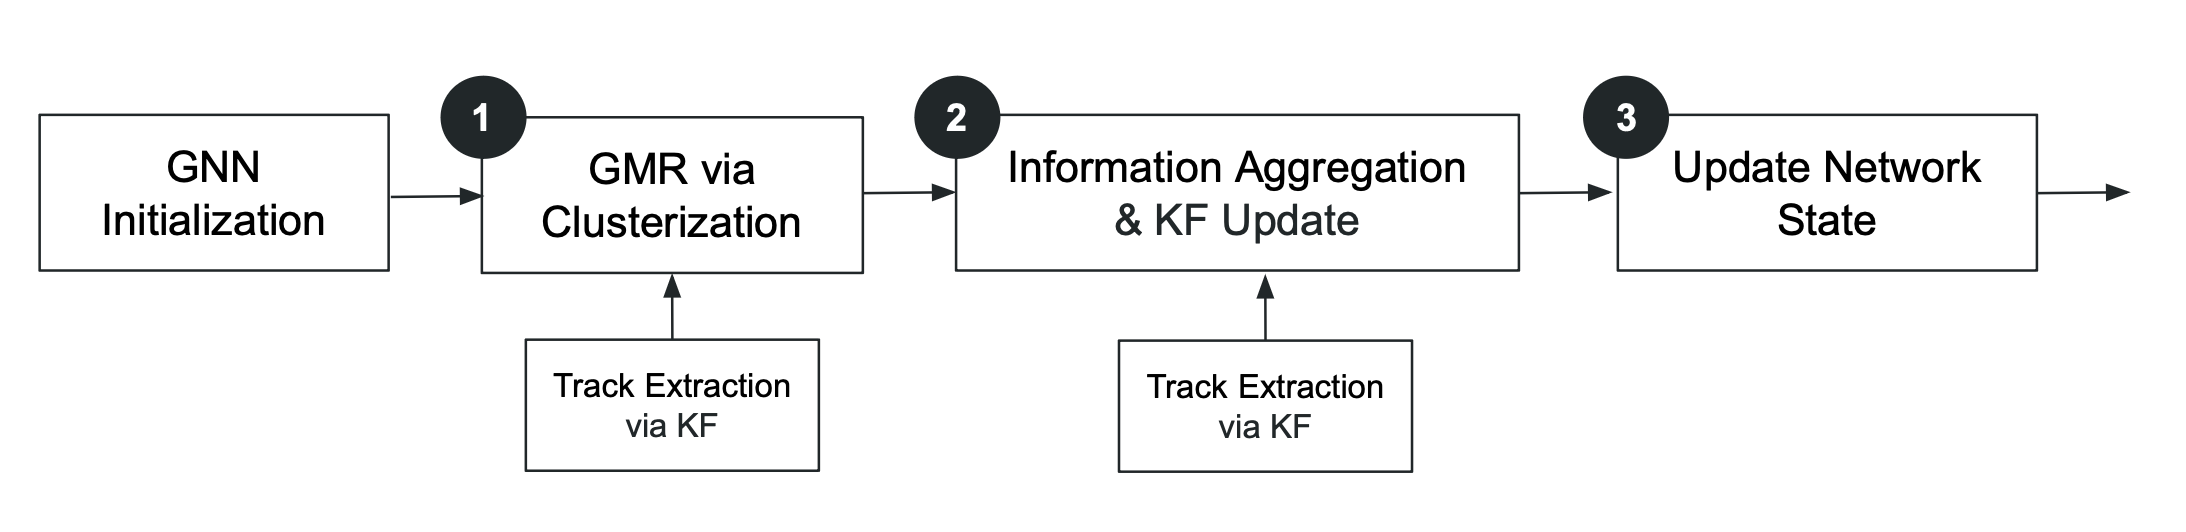
\includegraphics[width=0.98\textwidth]{images/5-gnn-algorithm/gnn-workflow.png}
    \caption{Flow chart illustrating all stages making up an iteration of the GNN-based algorithm. After each stage, a Kalman filter (KF) is applied in order to iteratively extract candidates. After stage three, a further Gaussian Mixture Reduction (GMR) stage would be applied repeating the iterations.}
    \label{fig:flowchart}%
\end{figure}


The first stage comprises of Gaussian Mixture Reduction (GMR). This involves a traditional ML approach, whereby compatible Gaussian states are grouped together using clustering techniques and outlier states can be identified. Following this, an Information Aggregation stage is executed, which leverages message passing between adjacent nodes in a given neighbourhood. The compatibility of neighbouring states can be assessed via extrapolation, in order to improve local track parameters using neighbourhood information. The third stage involves updating the network state at each node, as specific connections are deactivated as the network evolves. A graph splitting algorithm is also applied directly after the first two stages, in order to identify good track candidates, and if discovered they are extracted. 

Unlike traditional methodologies whereby MLPs are employed for deep learning strategies, the proposed GNN leverages simplified KFs embedded in the network which are used for two main purposes. Firstly, the KF is used as a mechanism for information propagation during the second stage, in order to iteratively improve the precision of track parameters. Secondly, the KF is used within the extraction of track candidates compatible with the particle motion model. This allows the algorithm to efficiently exploit a prior knowledge about charged particle dynamics as the network evolves.

The excitation and inhibition rules of individual edge connections are designed to facilitate the “simple-to-complex” approach for “hits-to-tracks” association, such that the network starts with low hit density regions of an event and gradually progresses towards more complex areas. As the network evolves, the uncertainty in local track parameters decreases until there are no more track candidates that fulfil the criteria for a good track. This is the end state of the network where isolated nodes, track fragments and unresolved ambiguities will remain.



\section{Graph Network Initialization}
\label{gnn-network-initialization}

The graph network is implemented using the Python library \texttt{NetworkX} \cite{SciPyProceedings_11}. Hits from a particle event are represented as nodes and predicted hit-pairs as edge connections. See Chapter \ref{chapter-4} for further details on the hit-pair predictor used to form edge connections. Following this, a common clustering technique, known as Connected Component Analysis (CCA), is applied using a built-in function of NetworkX \cite{networkx}. CCA detects connected regions in data structures and splits the network into smaller, more manageable, graphs referred to as \textit{subgraphs}. 

Each pairwise connection between node $i$ and neighbour node $j$ forms a Gaussian state, $X_{ij}$, representing the local track parameter estimate. Each edge has an associated prior probability $p_{ij}$ and edge weight $w_{ij}$. The prior probability of nodes $i$ and $j$ belonging to the same track is determined, assuming a track can produce at most one hit per detector layer. $w_{ij}$ is a mixture weight for the compatibility of the Gaussian state transmitted from node $i$ to neighbour node $j$, and represents the strength of the connection. The weights $w_{ij}$ are initialised uniformly and are dependent on the number of neighbours local to a node. The parameters $w_{ij}$ and $p_{ij}$ are updated as the network evolves. Note that, $w_{ij}$ are not to be confused with the traditional weights associated to features within neural networks. 

For a given node $i$ and neighbour nodes $j$, a Gaussian mixture $g_i(X)$ is formed from weighted components, $\Phi_{ij}$. A general form of $g_i(X)$ is given by Eq \eqref{eqn:gaussian-mixture},


\begin{equation}
g_i(X) = \sum_{j} w_{ij}\Phi_{ij}(X, X_{ij}, C_{ij})
\label{eqn:gaussian-mixture}
\end{equation}

where $C_{ij}$ are track state covariances. All edges act as bidirectional conduits, such that message passing can occur in both directions. All edges are initialised as \textit{active}, allowing the propagation of state information between its node-pair, whereas \textit{deactived} or \textit{non-active} edges are defined to not allow state information to be propagated. 

%Figure \ref{fig:network-initial} illustrates a node and its neighbourhood.

% \begin{figure}[htbp]%
%     \centering
%     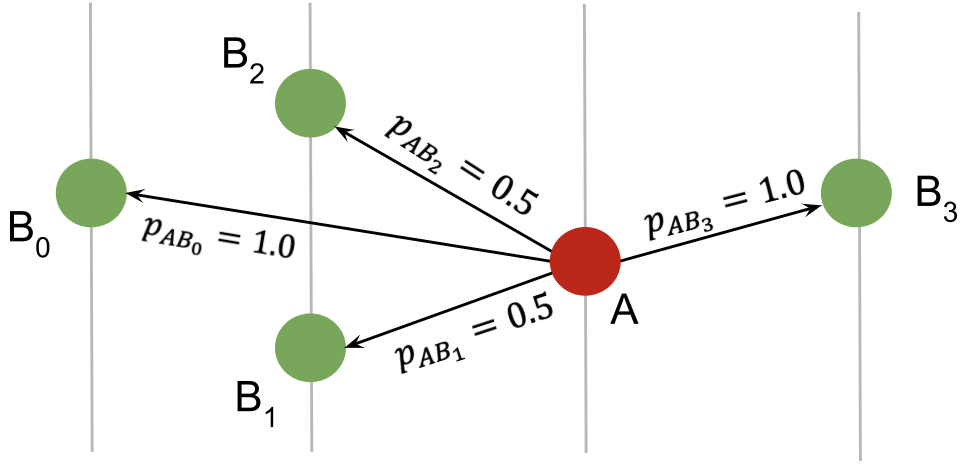
\includegraphics[width=8.8cm]{images/5-gnn-algorithm/network-initialisation.png}%
%     \caption{Prior probabilities associated to network edges of node A's local neighbourhood. Neighbours $B_j$ are located on separate detector layers shown by vertical lines. The unidirectional edges indicate the direction of propagation of state information and priors. These entities will differ from nodes $B_j$ distributing messages to their corresponding neighbourhoods.}%
%     \label{fig:network-initial}%
%\end{figure}




\section{Gaussian Mixture Reduction}
\label{section-GMR}

For nodes with a high multiplicity of edge connections, the number of potential track states can quickly rise. To make inferences within a reasonable amount of processing time, GMR is used to prevent the number of components from exploding. One computationally efficient algorithm for GMR is clustering. A high multiplicity Gaussian mixture can be approximated by one with lower multiplicity, using the traditional k-means clustering \cite{kmeans}. At each node, similar track states are grouped together forming a reduced mixture and their corresponding edges remain active, as illustrated in Figure \ref{fig:GMR-example}. 


\begin{figure}[htbp!] 
    \centering
    \subfloat[]{%
        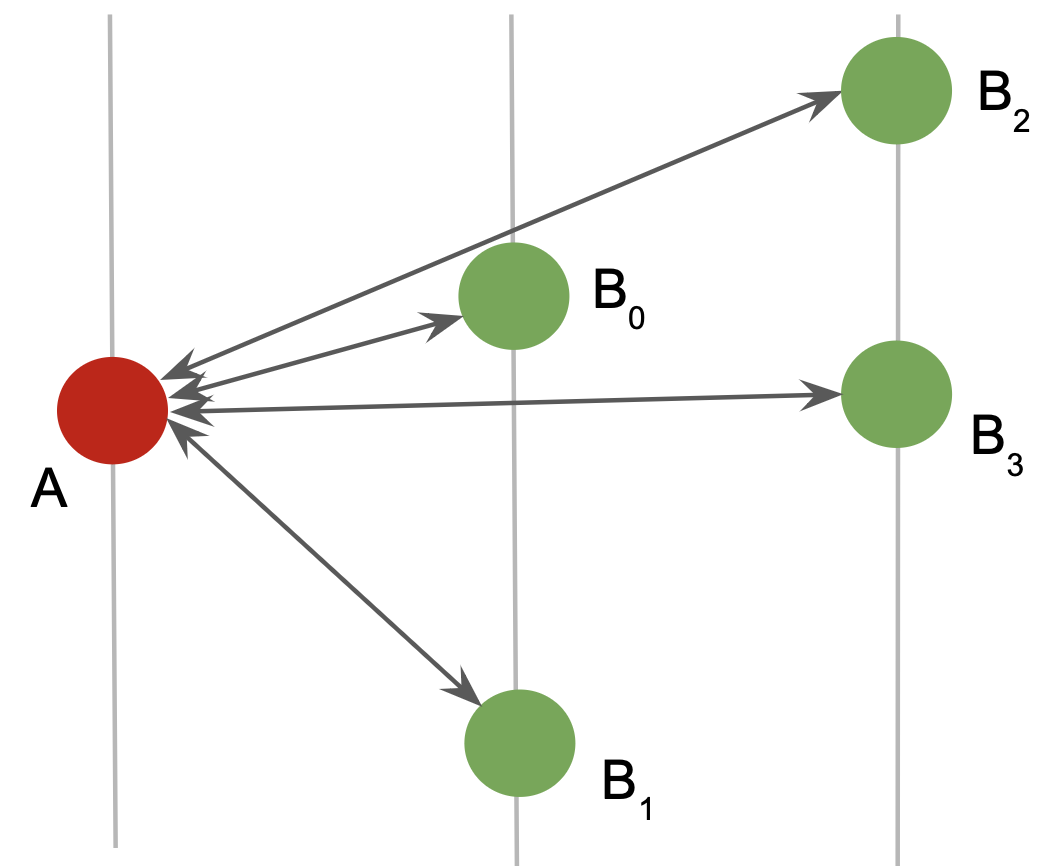
\includegraphics[width=0.42\linewidth]{images/5-gnn-algorithm/GMR-1.png}%
        \label{fig:GMR-1}%
        }%
    \hfill%
    \subfloat[]{%
        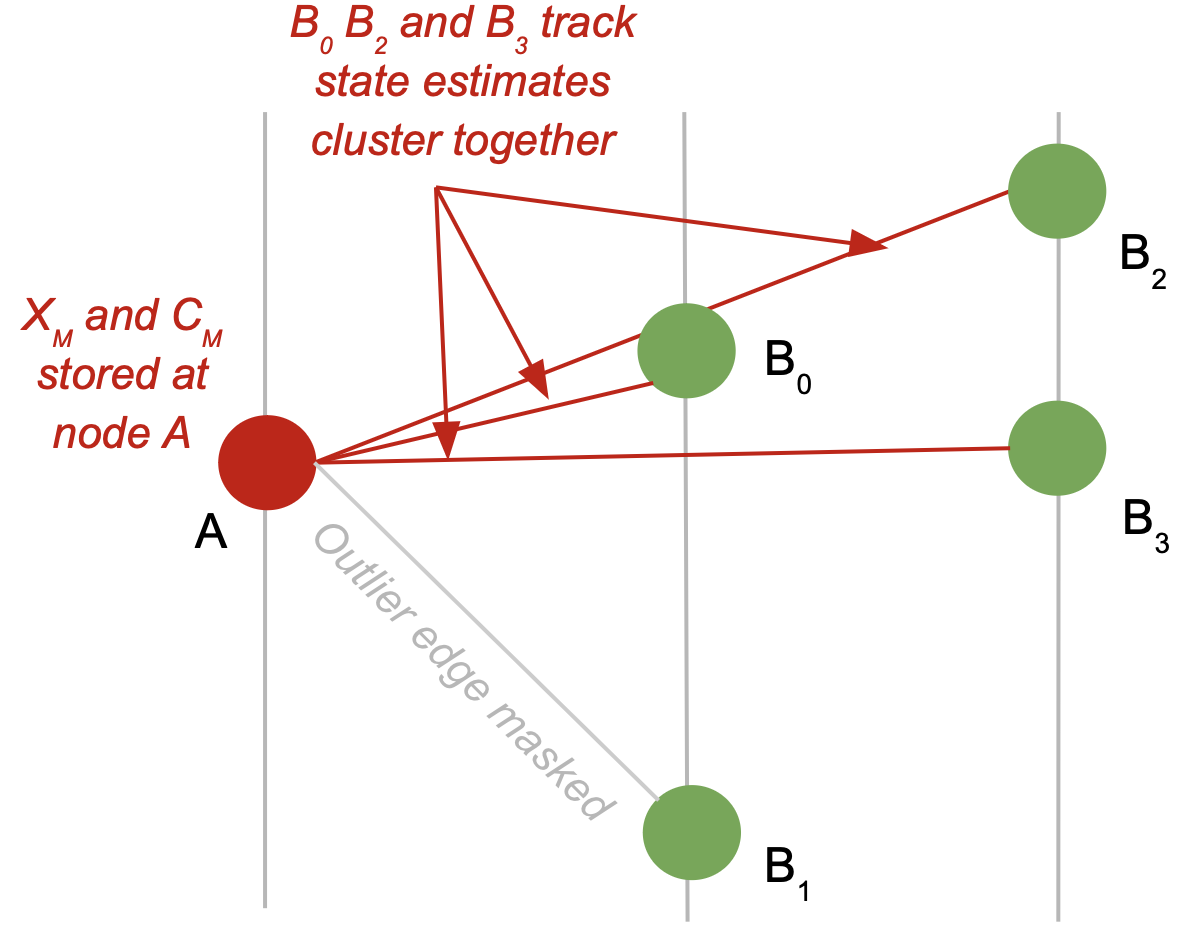
\includegraphics[width=0.57\linewidth]{images/5-gnn-algorithm/GMR-2.png}%
        \label{fig:GMR-2}%
        }%
    \caption{Illustration of GMR via clustering applied to graph networks.}
    \label{fig:GMR-example}
\end{figure}


Figure \ref{fig:GMR-1} shows node $A$ and its local neighbourhood $B_j$ with bidirectional edge connections. Figure \ref{fig:GMR-2} shows the expected result of GMR applied to node $A$. If clustering is successful, a merged track state estimate, $X_M$, is formed from states $X_{AB_0}$, $X_{AB_2}$, $X_{AB_3}$ clustered together and the corresponding merged state covariance, $C_M$, is formed from $C_{AB_0}$, $C_{AB_2}$, $C_{AB_3}$. Outlier states are simultaneously identified and their edges are deactivated. The incoming $B_1 - A$ edge has been deactivated (represented as a dotted line), as any incoming state information from neighbour $B_1$ is deemed incompatible at node $A$.

The merged state estimate $X^{M}$ and merged state covariance $C^{M}$ are computed using the inverse-variance weighting \cite{inverse-variance-weighting} given by Eq \eqref{eqn:inverse-variance-weighting}, where $G_{ij}$ = $C_{ij}^{-1}$.

\begin{equation}
    X^{M} = C^{M} \sum_{j} G_{ij} X_{ij},  \quad  C^{M} = \left( \sum_{j} G_{ij} \right) ^{-1}
    \label{eqn:inverse-variance-weighting}
\end{equation}

The k-means clustering is implemented using the general case of $k=1$, to model the Gaussian mixture at each node as a single track with outlier connections. For the case where a node is located in close proximity to an intersection between two tracks, two or more clusters can be expected. In such a case, the mixture reduction process is declared impossible. This part of the network remains dormant until competing edges are deactivated through information propagation from other parts of the network and the mixture becomes more unimodal. 


\subsection{The Kullback-Leibler Divergence}
In order to establish whether clustering can occur for a given node, a distance measure is used as a threshold. The Kullback-Leibler (KL) divergence, $d_{KL}$, is a measure of the statistical distance between two Gaussian probability distributions \cite{KL, FRUHWIRTH19971}, and is used in the k-means algorithm to determine if track states can be grouped into a cluster. The $d_{KL}$ between $X_{ij}$ and $X_{ik}$ is given by Eq \eqref{eqn:kullback-leibler}.

\begin{equation}
    d_{KL} = tr[(C_{ij} - C_{ik})(G_{ij} - G_{ik})] + (X_{ij} - X_{ik})^{T}(G_{ij} + G_{ik})(X_{ij} - X_{ik})
    \label{eqn:kullback-leibler}
\end{equation}

The optimal $d_{KL}$ threshold will differ for each node depending on its local neighbourhood. For example, consider a node with a high empirical variance of edge orientation in its neighbour connections, $\sigma_{e}^{2}$. The corresponding $d_{KL}$ threshold will be larger in comparison to a node with a small $\sigma_{e}^{2}$, where neighbour connections are more closely orientated. To determine the optimal $d_{KL}$ threshold between pairwise $X_{ij}$ for a given node, a SVM classifier was trained against truth information using a MC simulation. See Section \ref{chapter-6-kl-threshold} for further details on the implementation.





\section{Information Aggregation}

\subsection{Message Passing}
The message passing mechanism of graph networks is leveraged in order to improve the precision of track state parameters on a local and global scale. During the previous stage (Section \ref{section-GMR}), reduced Gaussian mixtures were formed for nodes where clustering was successful. For a given node $i$, $X^M$ and $C^M$ are propagated to all neighbours $j$ which have active $i \rightarrow j$ connections. If clustering was unsuccessful for a particular node, this part of the network remains dormant until a merged state is received via message passing during later stages of the algorithm. Track state information can be propagated in both directions along active network edges. This ensures that the compatibility of received states can be validated and assessed against each node's local neighbourhood.


\subsection{Validation}
Once state information has been propagated to neighbours, the parameter estimation begins with a linear projection of the incoming track state onto the subspace of measurements. As illustrated in Figure \ref{fig:extrapolation}, for a given node $i$ each incoming $X^M$ is projected via a measurement matrix $H$, which relates the incoming track state to the measurement values. See Section \ref{gnn-application-toy-model} for implementation of matrix $H$. In order to validate if the connection between node $i$ and $j$ is compatible, the Mahalanobis distance, $\Delta \chi^{2}_{ij}$, is calculated using the residual between the projected state, $HX$, and the measurement at the neighbour node, $m$. The threshold $d_{\chi^{2}}$ is a tuned hyperparameter and represents the maximum $\Delta \chi^{2}_{ij}$ acceptable for an incoming track state. If $\Delta \chi^{2}_{ij} \leq d_{\chi^{2}}$, the connection is deemed compatible and the state can be extrapolated via a KF. If $\Delta \chi^{2}_{ij} > d_{\chi^{2}}$ then the connection is deemed incompatible and the corresponding edge is deactivated.

\begin{figure}[htbp]
        \centering
        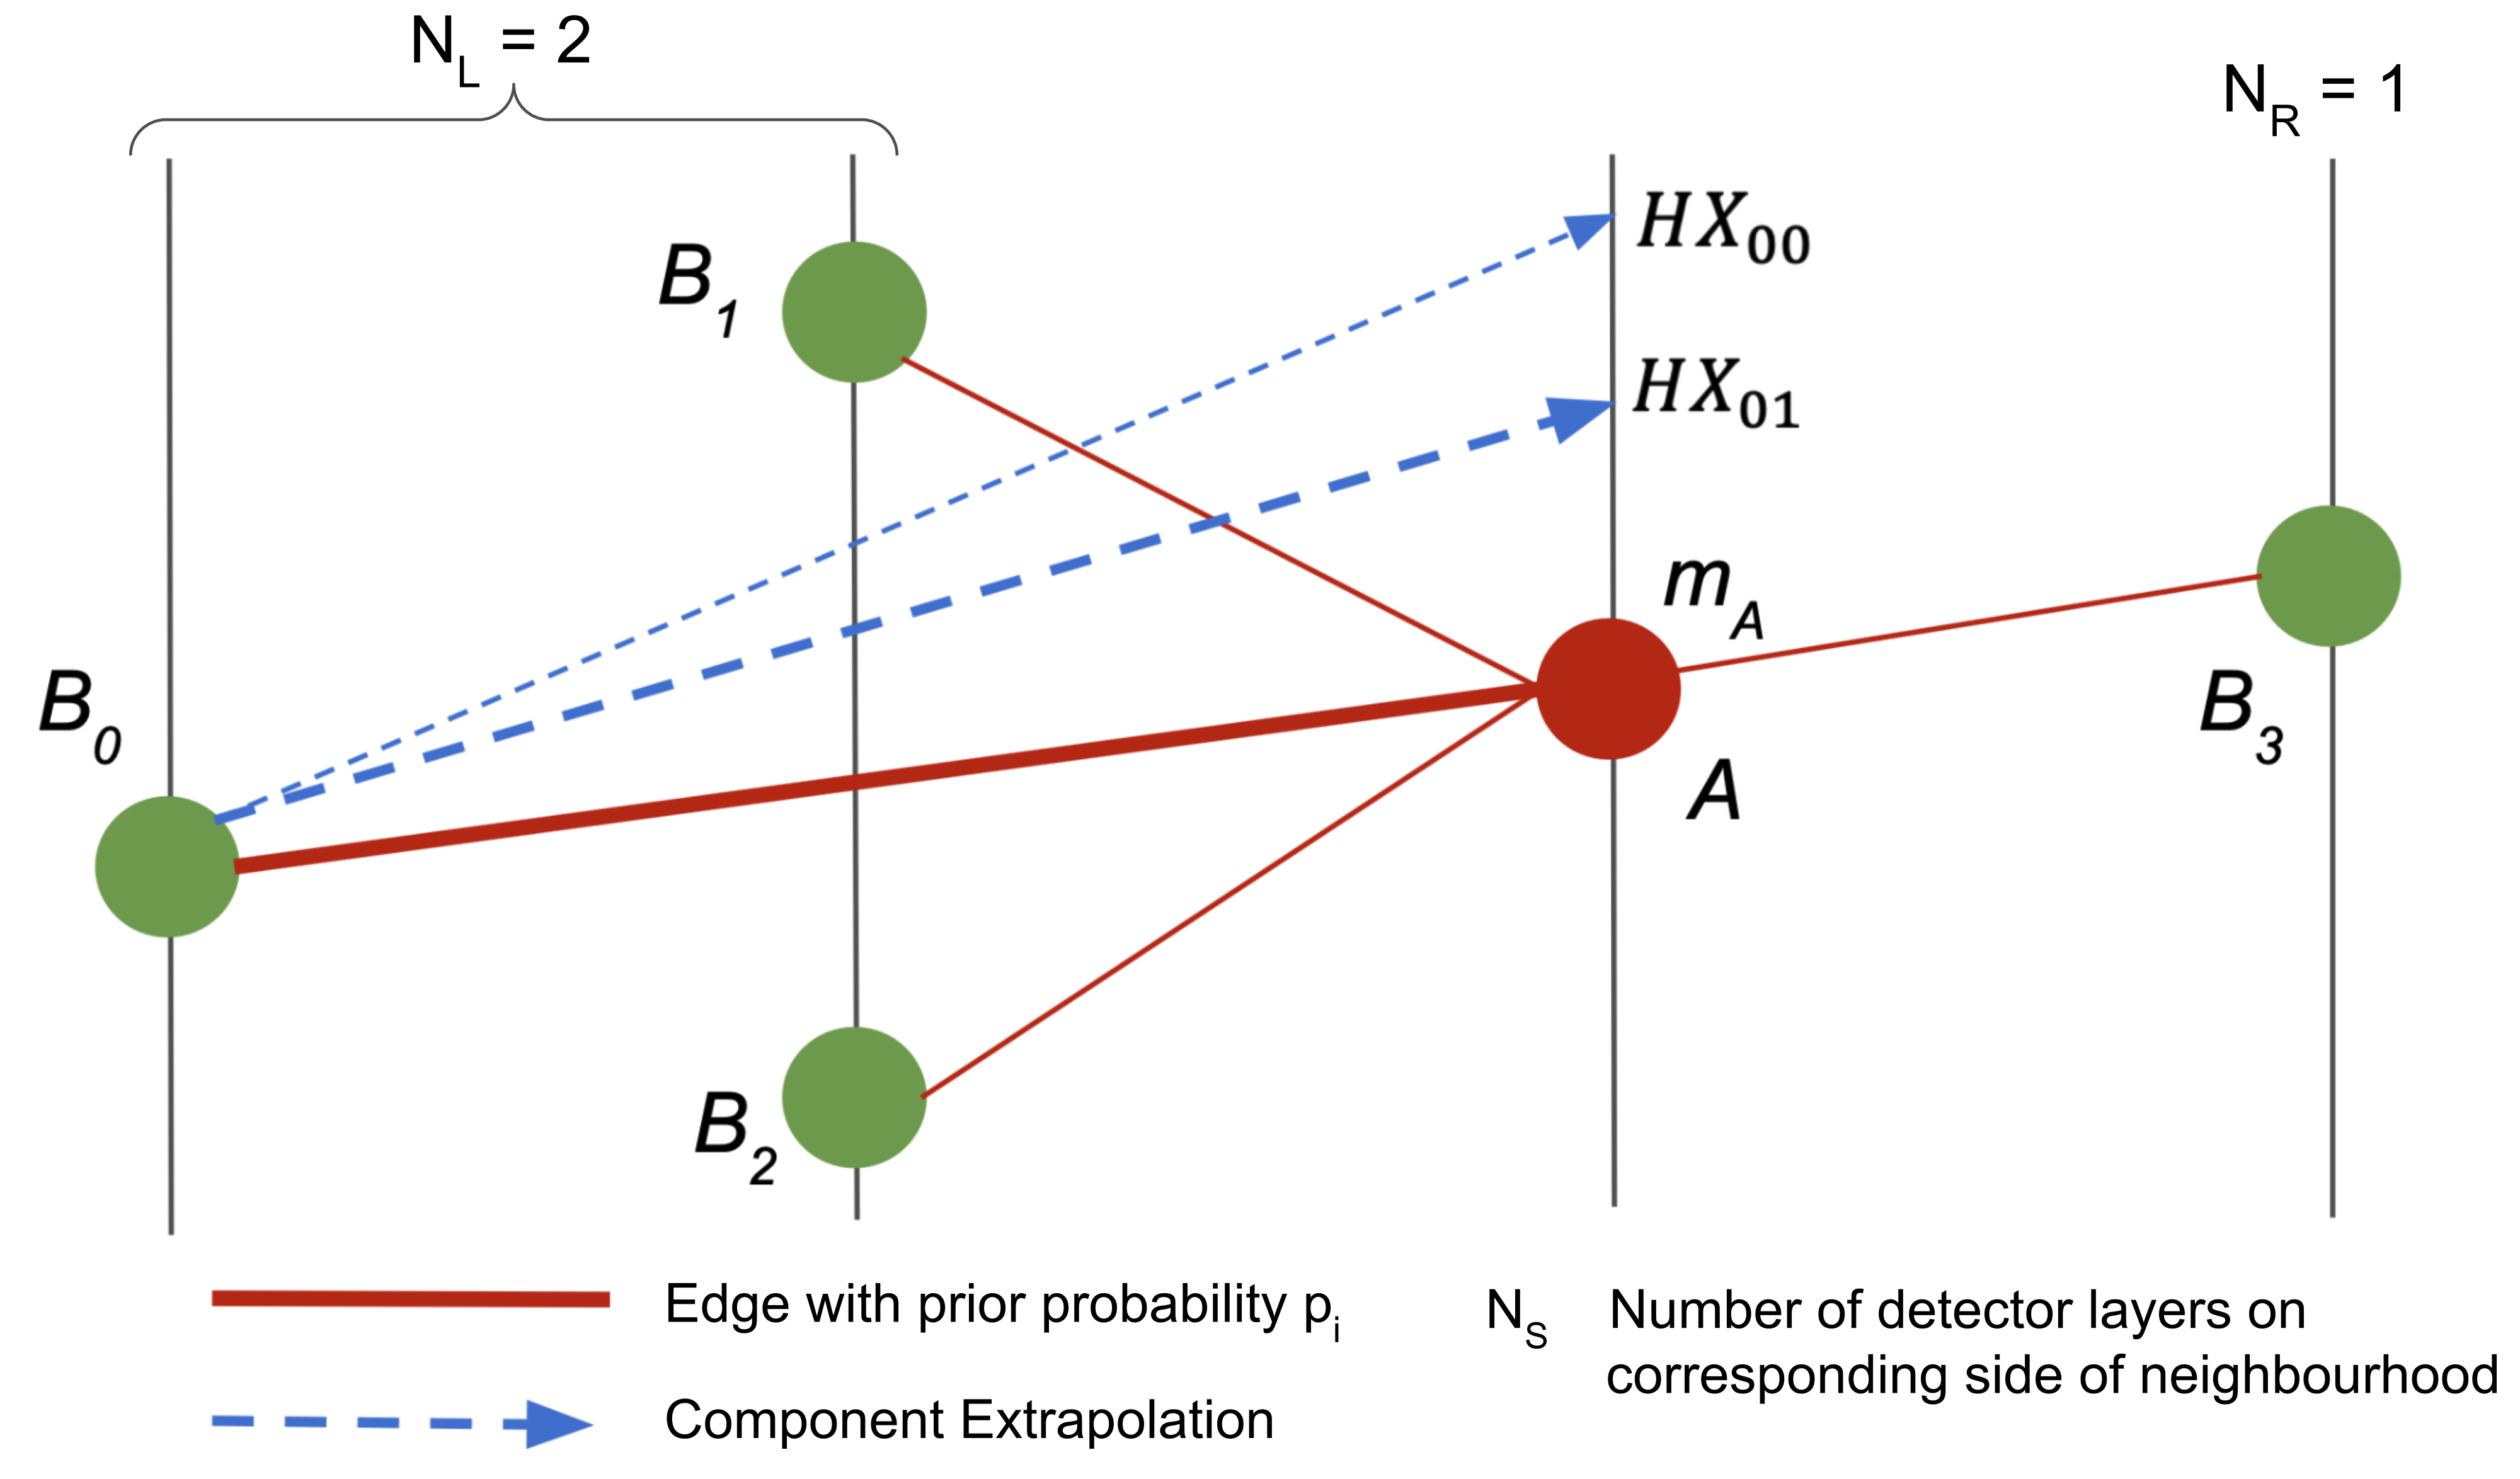
\includegraphics[width=0.87\textwidth]{images/5-gnn-algorithm/gnn-extrapolation.png}
        \caption{Illustration of track state estimates $X_{00}$ and $X_{01}$ being projected from node $B_0$ to node $A$ via a measurement matrix $H$ into the subspace of measurements. $m_A$ is the measurement at node $A$. The corresponding residual between $m_A$ and the projected incoming state from $B_0$ is used to compute the Mahalanobis distance $\Delta \chi^{2}$ to determine if the incoming state is compatible with $m_A$. $N_L$ indicates the number of detector layers on the left side of node $A$'s local neighbourhood, and $N_R$ indicates the number of detector layers on the right side.}
        \label{fig:extrapolation}%
\end{figure}


\subsection{KF Update and Extrapolation}
\label{chapter-5-kf-extrapolation}

For compatible incoming states where $\Delta \chi^{2}_{ij} \leq d_{\chi^{2}}$, the KF update is applied in order to compute the extrapolated track state estimate, $\tilde{X}_{ij}$, and the corresponding extrapolated covariance matrix, $\widetilde{C}_{ij}$. The KF is implemented via the Python library \texttt{Filterpy} \cite{filterpy}. $\tilde{X}_{ij}$ and $\widetilde{C}_{ij}$ are given by Eqs. \eqref{eqn:extrapolation},

\begin{equation}
\tilde{X}_{ij} = F_{ij} X_{ij}^{M}, \qquad \tilde{C}_{ij} = F_{ij} \biggl( \sum C_{ij}^{M} + Q_{ij} \biggl) F^{T}_{ij}
\label{eqn:extrapolation}
\end{equation}

where $F_{ij}$ is the state transition Jacobian from node $i$ to node $j$, and $Q$ is the process noise matrix. See Section \ref{gnn-application-toy-model} for implementation of the KF update, including the transition Jacobian $F$ and process noise $Q$. 






\section{Updating Network State}
\label{gnn-updating-network-state}

As the network evolves and specific connections are deactivated, the local track parameter estimates change at each node. Therefore, the corresponding edge weights, $w_{ij}$, should reflect this for the strength of each connection, and hence $w_{ij}$ are updated. For the connection between nodes $i$ and $j$, the updated edge weights $\widetilde{w}_{ij}$ are computed using the normalised Gaussian measurement likelihood given by Eq \eqref{eqn:likelihood}, where $S_{ij}$ is the joint measurement covariance matrix.

\begin{equation}
\beta_{ij} = (2 \pi \lvert S_{ij} \rvert )^{-1/2}  e^{-\Delta \chi^{2}_{ij} / 2}
\label{eqn:likelihood}
\end{equation}


The updated edge weights $\widetilde{w}_{ij}$ are given by Eq \eqref{eqn:weights}. 

\begin{equation}
\widetilde{w}_{ij} = \frac{1}{N_S} \frac{w_{ij}\beta_{ij} p_{ij}}{\sum_{k}w_{ik}\beta_{ik}}
\label{eqn:weights}
\end{equation}


The denominator $\sum_{k}w_{ik}\beta_{ik}$ is the summation of the product of weights and likelihoods in the neighbourhood of a given node $i$. The weights $\widetilde{w}_{ij}$ are also divided by the number of detector layers on either side of its neighbourhood, $N_S$, in order to account for the probability that a track passing through node $i$ was detected at layer $L$. If $\widetilde{w}_{ij} < 0.1$, the corresponding edge connection is automatically deactivated as the likelihood of compatibility of this incoming track state is extremely low. This forms part of the mechanism for edge activation and deactivation.

The Gaussian mixture $g_i(X)$ at each node is then composed of updated components, given by Eq \eqref{eqn:updated-gaussian-mixture}.

\begin{equation}
g_i(X) = \sum_{j} \widetilde{w}_{ij}\Phi_{ij}(X, \widetilde{X}_{ij}, \widetilde{C}_{ij})
\label{eqn:updated-gaussian-mixture}
\end{equation}

Following this update, the algorithm iterations repeat. A further GMR would follow, clustering on $\widetilde{X}_{ij}$. This allows further ambiguities to be resolved and the precision of track state parameters to be increased at each additional stage.






\section{Graph Splitting and Track Extraction}
\label{gnn-track-extration}

The design of the GNN-based framework is such that it is possible to iteratively discover track candidates after each stage. As shown in Figure \ref{fig:flowchart}, a track extraction algorithm is executed after the GMR and Information Aggregation stages.

Initially, the graph network must be split into smaller components, taking into account only edges which remain active. A CCA is applied to the network by using the NetworkX built-in function \texttt{weakly\_connected\_components}. This ensures that smaller, more manageable subgraphs are separated from the main network.

The criteria that a subgraph must possess in order to be considered for track extraction are as follows. Subgraphs must contain a minimum number of four nodes within the volume of interest. There must exist only one node per detector layer, so that there are no are intersecting tracks or holes within the track candidate. 

If the above criteria are met, a KF is then applied in order to perform a final track fit. As opposed to applying the KF on one track segment between two nodes, similar to the method used in Section \ref{chapter-5-kf-extrapolation} for state extrapolation, the KF for track fitting considers the whole chain of track segments. Here, the filter iteratively predicts and updates track state parameters as it receives measurements from each subsequent node in the subgraph. The KF is initialised with a filter state estimate, $\hat{x}$, a filter state covariance, $\hat{P}$, state transition Jacobian, $\hat{F}$, measurement function, $\hat{H}$, measurement noise $\hat{R}$ and process noise, $\hat{Q}$.

In order to assess the quality of the track fit the p-value is computed from the $\chi^2$ statistic. The p-value obtained must be greater than 0.01. Subgraphs that fulfill all conditions are defined as good track candidates and are extracted from the network, such that their corresponding nodes and edges are removed. Subgraphs that do not meet the above criteria for track extraction, remain in the graph network for further processing.





\section{Application on a Simple MC Model}
\label{gnn-application-toy-model}

A linear 2-dimensional model was used to simulate seven truth tracks in the $x$-$y$ plane, each with ten hits as shown in Figure \ref{fig:ground-truth}. 

\begin{figure}[htbp]
    \centering
    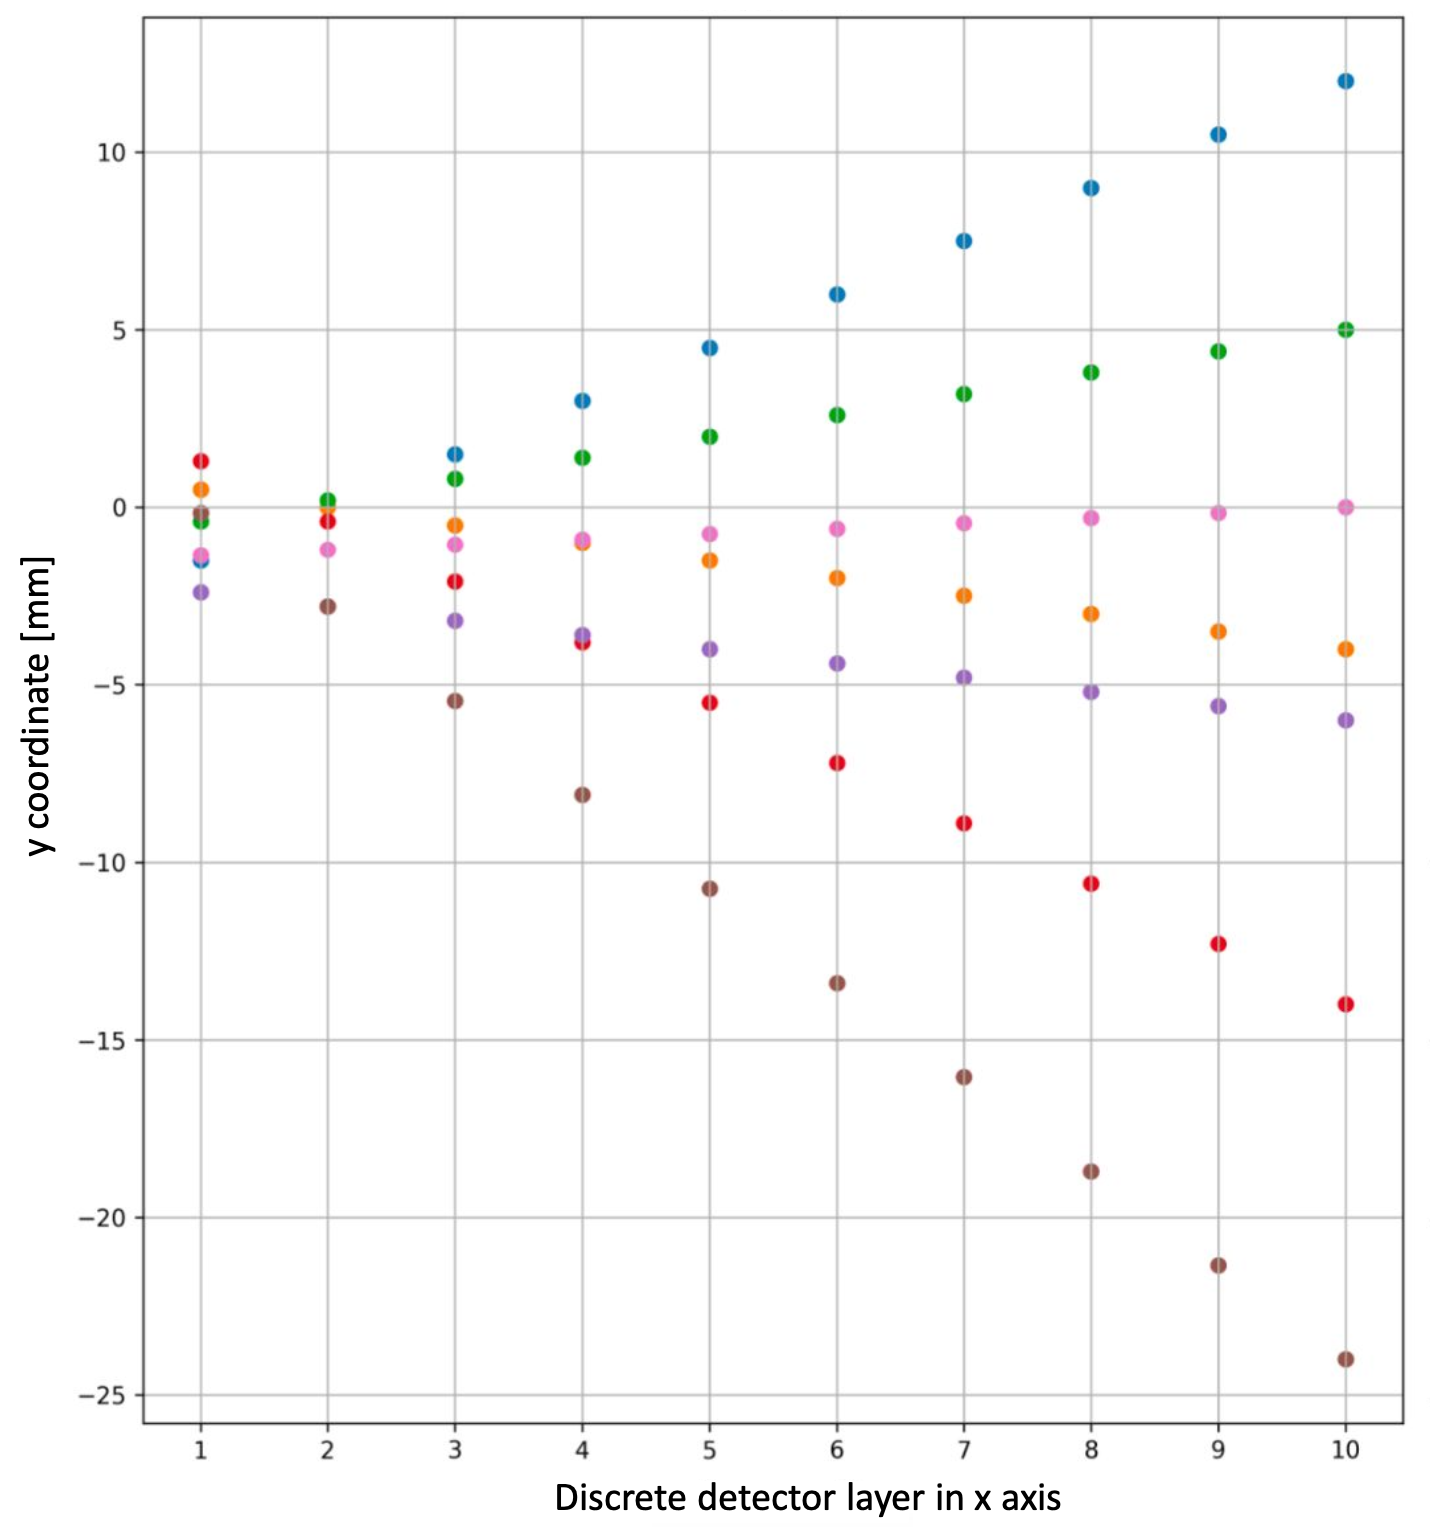
\includegraphics[width=0.55\textwidth]{images/5-gnn-algorithm/ground-truth.png}
    \caption{Simulation of seven truth tracks.}
    \label{fig:ground-truth}%
\end{figure}

Random Gaussian noise was added to the $y$-coordinate in order to simulate measurement error. The track position measurements, $m$, are given by Eq \eqref{eqn:mc-toy-measurement-model}

\begin{equation}
m = y + \sigma_0 \eta
\label{eqn:mc-toy-measurement-model}
\end{equation}

where $y$ is the unobserved track positions, $\sigma_0$ is the standard deviation in the measurement of the $x$-$y$ plane and is initialised to $100 \mu $m, and $\eta$ is a Gaussian random variable with zero mean and variance of one.

The graph network was formed using a many-to-one mapping of hits-to-nodes, where hits in close proximity within each layer were merged into one node. The threshold for the merging was determined using the distance distribution between hits located in the same layer. To build edge connections and reduce all possible combinatorics between node pairs, an edge-predictor method was devised. The predictor uses the track inclination of neighbour nodes. If the inclination of a neighbour node spanning up to two layers apart is within a particular range, this edge is deemed compatible and a connection is established. 

The node degree (the number of edges associated to each node) and the empirical variance of edge orientation in its neighbour connections, $\sigma_{e}^{2}$, provide indications of neighbourhood complexity. For example, nodes which have a high multiplicity of connections indicate areas where there are significant outliers to resolve, and vice versa for nodes with low degree. This feature is illustrated by Figure \ref{fig:heat-map}, which shows a heat map labelled by node degree. High degree nodes are referred to as ``hot'' (white-yellow) and low degree nodes are referred to as ``cold'' (orange-red).


\begin{figure}[htbp]
    \centering
    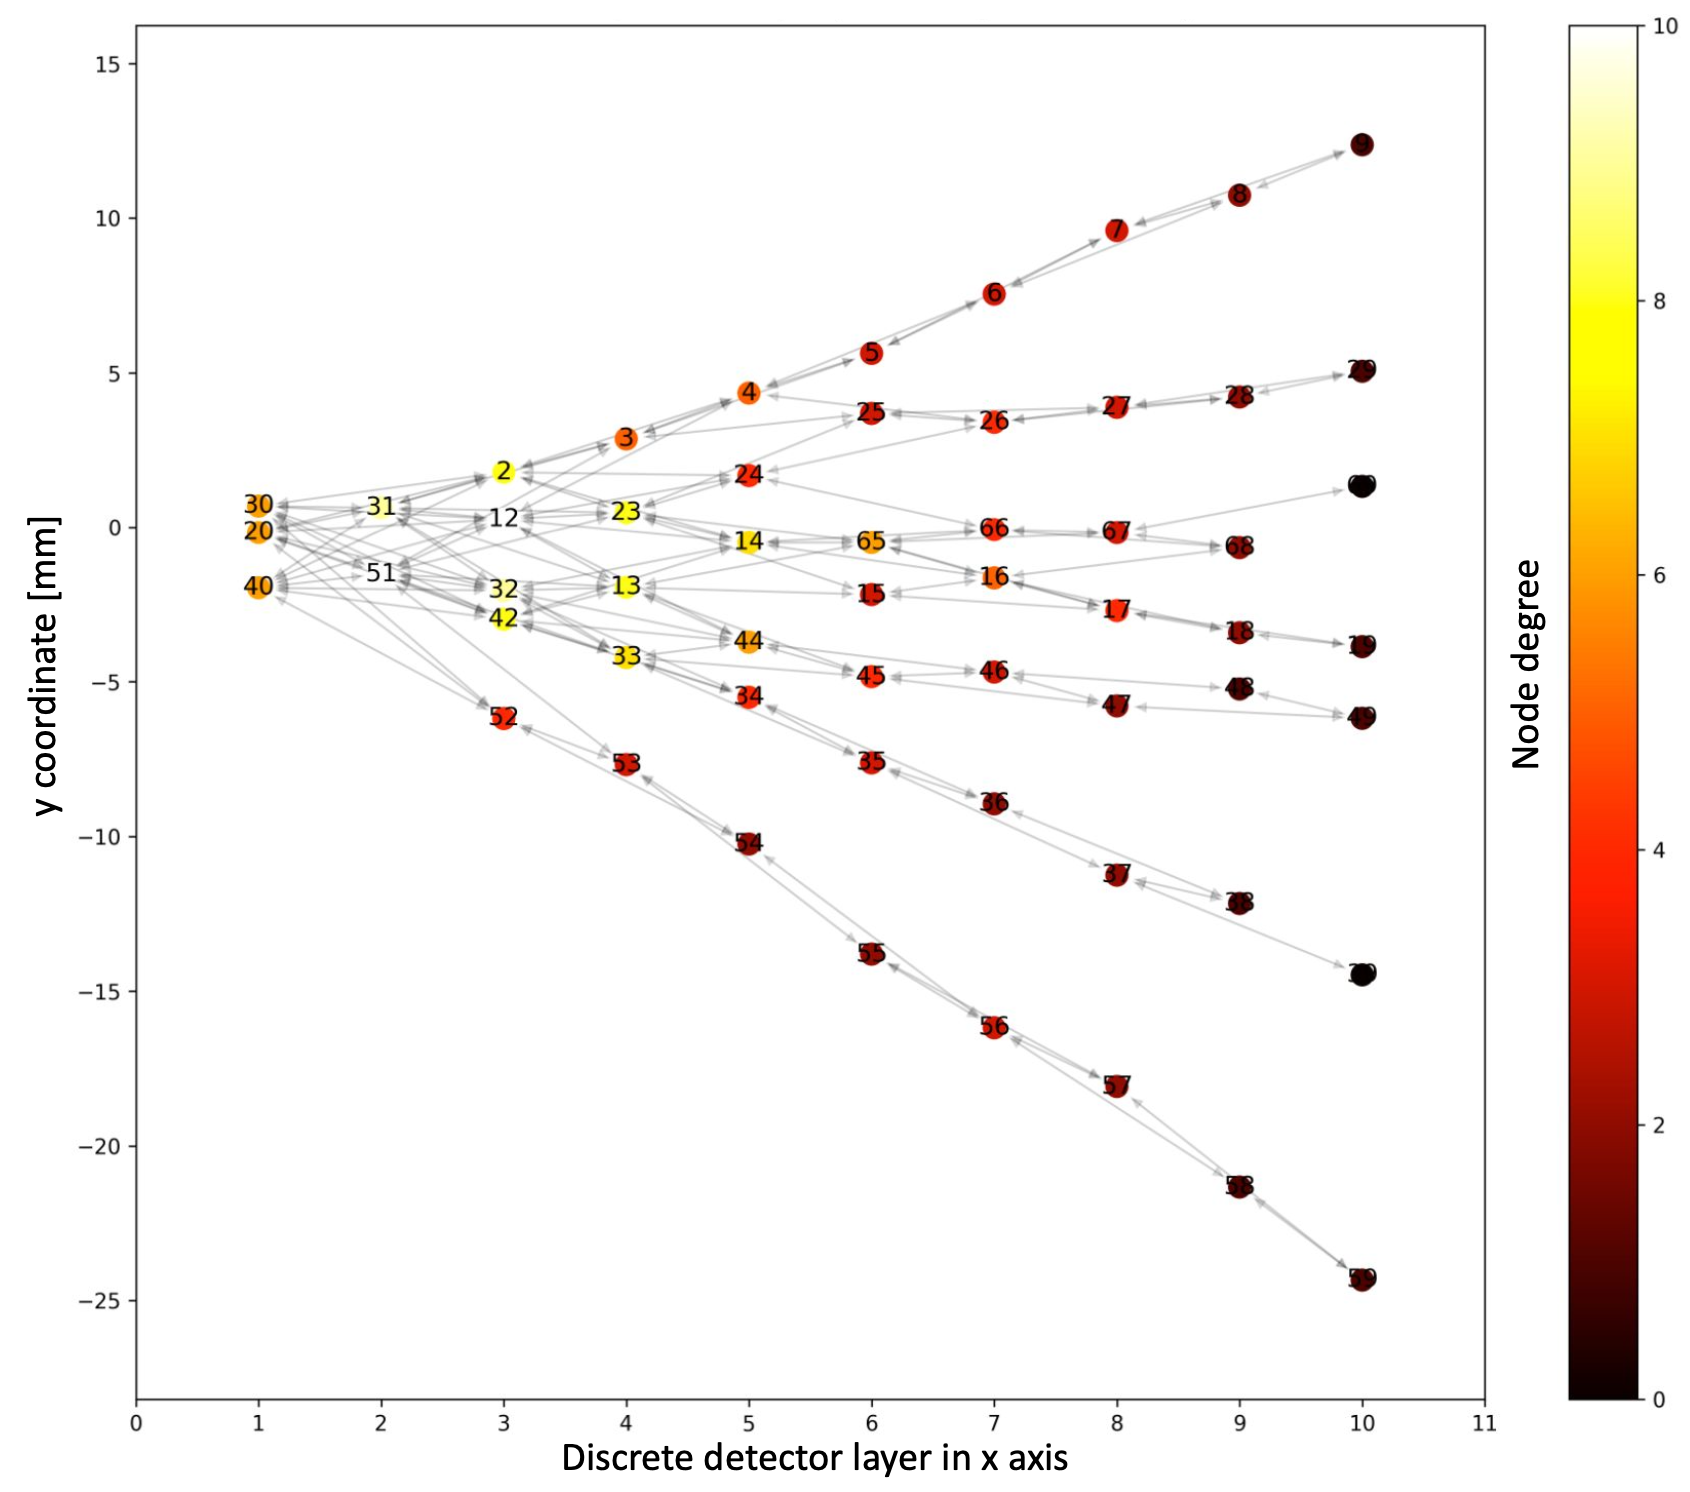
\includegraphics[width=0.85\textwidth]{images/5-gnn-algorithm/heatmap-network.png}
    \caption{Conversion of simulated hits in Figure \ref{fig:ground-truth} to a graph network, plotted as a node-degree heat map using the model in Eq \eqref{eqn:mc-toy-measurement-model}. Edge connections are formed using a pair predictor. The heat map represents node degree, where ``hot'' nodes (white-yellow) contain many edge connections, whereas ``cold'' nodes (orange-red) contain fewer edge connections.}
    \label{fig:heat-map}%
\end{figure}


\subsubsection{Graph Network Initialization}

The network is initialised with track state estimates, $X_{ij}$, given by Eq \eqref{eqn:track-state-estimate} and MC truth particle at each node. Each connection is modelled as a straight line, where $X_{ij}$ comprises of the $y$-measurement at node $i$, given by $m_i$, and the track inclination to its neighbour node $j$, given by $\tau_{ij} = (m_i - m_j) / (x_i - x_j)$, so that

\begin{equation}
X_{ij} = \begin{bmatrix} m_i \\ \tau_{ij} \end{bmatrix}
\label{eqn:track-state-estimate}
\end{equation}


The joint measurement covariance matrix, $S$, is stated in Eq. \eqref{eqn:track-state-estimate-2}, where $\sigma_0 = 100\mu$m. Negligible error is assumed in the $x$-measurement due to the low thickness of Pixel sensors. The state covariance, $C_{ij}$, is derived using the standard linear algebra approach, where $C_{ij} = GSG^T$, where matrix $G$ relates the measurements to the state vector, $X_{ij}$, using a linear extrapolation, where $dx = x_i - x_j$.  

\begin{equation}
S = \begin{bmatrix} \sigma_0^{2} & 0 \\ 0 & \sigma_0^{2} \end{bmatrix}  \quad G = \begin{bmatrix} 1 & 0 \\ dx^{-1} & -dx^{-1}  \end{bmatrix}
\label{eqn:track-state-estimate-2}
\end{equation}


\subsubsection{Implementation of Track State Extrapolation}

During Stage 1: GMR, $X^{M}$ and $C^{M}$ are computed using Eq \eqref{eqn:inverse-variance-weighting}. During Stage 2: Information Aggregation, $X^M$ is projected into the subspace of measurements using the measurement vector $H = [1 \quad 0]$. The residual, $r_{ij}$, between the projection, $HX^M$, and the measurement at each node is calculated using Eq \eqref{eqn:residual}

\begin{equation}
r_{ij} = m_i - HX_{ij}^M
\label{eqn:residual}
\end{equation}

The covariance of the residual, $V_{ij}$, is given by Eq. \eqref{eqn:covariance-of-residual}

\begin{equation}
{V}_{ij} = H \widetilde{C}_{ij} H^{T} + \sigma_{0}^{2}
\label{eqn:covariance-of-residual}
\end{equation}

where the extrapolated covariance, $\widetilde{C}_{ij}$, is calculated using Eq \eqref{eqn:extrapolation} with process noise, $Q$, defined as the zero matrix. The corresponding Mahalanobis distance is given by Eq \eqref{eqn:mahalanobis-distance}, and the distribution can be seen in Figure \ref{fig:mahalanobis-threshold-toy-model}.

\begin{equation}
\Delta \chi_{ij}^{2} = r_{ij}^{T} {V}_{ij}^{-1} r_{ij}
\label{eqn:mahalanobis-distance}
\end{equation}


\begin{figure}[htbp]
    \centering
    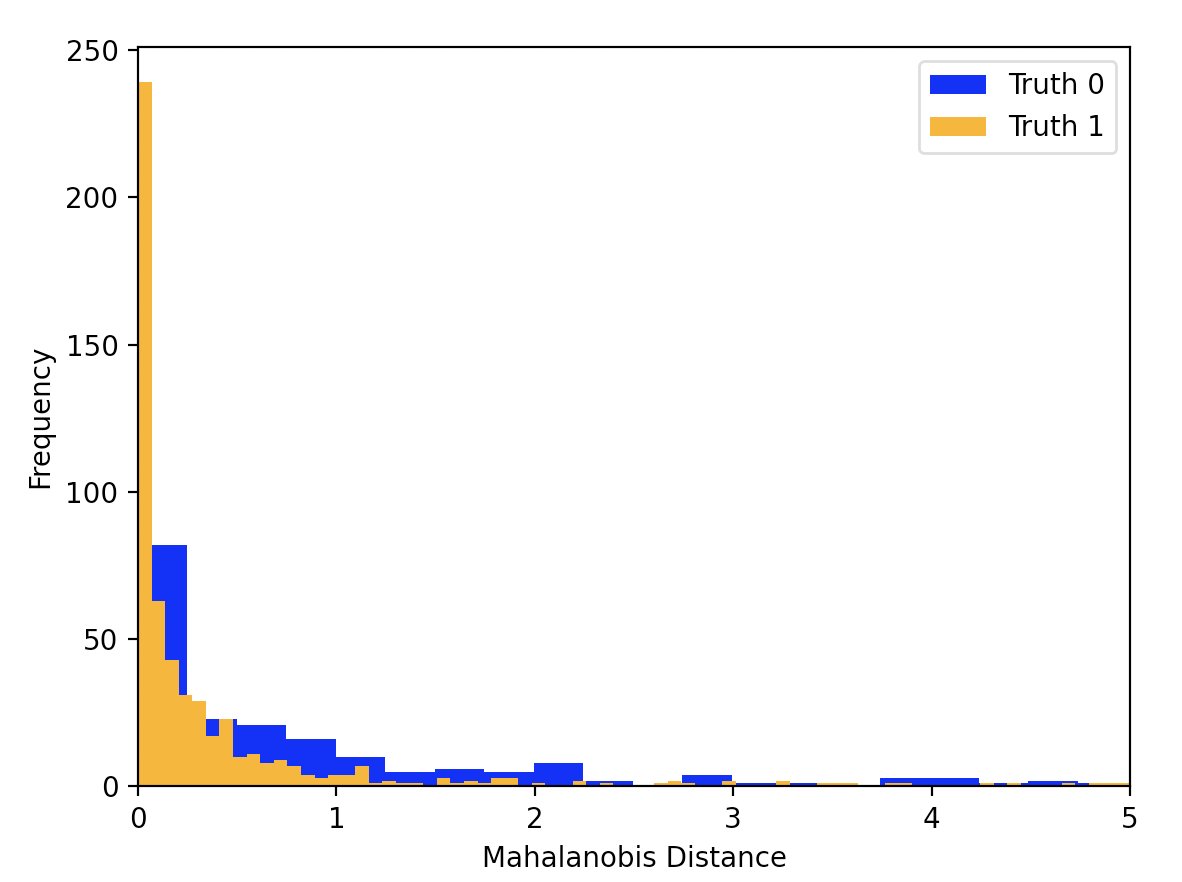
\includegraphics[width=0.85\textwidth]{images/5-gnn-algorithm/mahalanobis-threshold-toy-model.png}
    \caption{Mahalanobis distance, $\Delta \chi^{2}$, computed between the projected state and the measurement at each node, during state extrapolation for the GNN algorithm applied to a simple toy MC model. Truth 1 shows the distribution where the truth particle originating from the extrapolated state and the truth particle originating from the measurement are the same, and truth 0 otherwise.}
    \label{fig:mahalanobis-threshold-toy-model}%
\end{figure}



Using Figure \ref{fig:mahalanobis-threshold-toy-model} a distance of 1.0 is selected as a threshold for accepting extrapolated states, as this provides 95\% efficiency on selecting the truth 1 class. If $\Delta \chi_{ij}^{2} < 1.0$, then $X^M$ is extrapolated to its neighbour node using the KF update. The extrapolated state, $\widetilde{X}_{ij}$, is calculated by the KF using \eqref{eqn:extrapolation} defined as the linear extrapolation from node $j$ to node $i$. This is described by $m_i = m_j + \tau_j dx$ and $\tau_i = \tau_j$. Therefore, the derived Jacobian, $\hat{F}$, for the KF is given by Eq \eqref{eqn:mc-model-F}.

% Jacobian F is derived by differentation of m_i and t_i equations with respect to initial parameters m_j and t_j

\begin{equation}
\hat{F} = \begin{bmatrix} 1 & dx \\ 0 & 1 \end{bmatrix}
\label{eqn:mc-model-F}
\end{equation}



\subsubsection{Implementation of KF for Track Extraction}

For a set of $n$ nodes representing a track candidate, the sequential set of measurements are $\{m_{(n-1)}, ..., m_1, m_0 \}$, where $m_{(n-1)}$ is the measurement of the node with the largest radius. The KF for track extraction is initialised with the following two-dimensional filter state estimate, $\hat{x}$, given by Eq \eqref{eqn:kf-toy-model-x-init}.

\begin{equation}
\hat{x} = \begin{bmatrix} m_{(n-1)} \\ \tau_{(n-1)} \end{bmatrix}
\label{eqn:kf-toy-model-x-init}
\end{equation}

where the track position measurement, $m_{(n-1)}$, is known and the track inclination, $\tau_{(n-1)}$, is initialized to zero as track inclination information is unknown at the start of the filter. The filter covariance matrix, $\hat{P}$, is initialised using Eq \eqref{eqn:mc-model-P-init-covariance}

\begin{equation}
\hat{P} = \begin{bmatrix} \sigma_0^{2} & 0 \\ 0 & \sigma_{\tau}^2 \end{bmatrix}
\label{eqn:mc-model-P-init-covariance}
\end{equation}

where $\sigma_{\tau}^2$ is the variance in the track inclination, $\tau$, and is initialized to $10^3$. The measurement error in the KF, $\hat{R}$, is attributed to the error due to the measurement of the $x$-$y$ plane and is initialised to $\sigma_{0} = 100\mu$m. The transition Jacobian in the KF uses the linear model and is given by Eq \eqref{eqn:mc-model-F}. The measurement vector is given by $\hat{H} = [1 \quad 0]$ and the process noise matrix is set to $\hat{Q} = 0$.



\subsubsection{Results}

Figure \ref{fig:example-application-1} shows an example of the GNN algorithm applied to the simulated network in Figure \ref{fig:heat-map}. Figure \ref{fig:mc-example-1} displays the graph network where an initial CCA has been applied. Three smaller subgraphs have been identified as shown by separate colours. Nodes with $\sigma_e^2 > 0.8$ are not shown as clustering was not possible. The subsequent extracted track candidates are shown in Figure \ref{fig:mc-example-2}, where seven distinct tracks are observed and outlier edge connections have been successfully identified. This simulation shows 100\% efficiency of track reconstruction with respect to MC truth, as all seven truth tracks were extracted in two stages. 

Figure \ref{fig:example-application-2} shows another simulation of the MC toy track model with application of the GNN algorithm. The application of CCA yields two distinct subgraphs shown in Figure \ref{fig:mc-example-3} by two separate colours. The subsequent extracted track candidates are shown in Figure \ref{fig:mc-example-4}, where six distinct tracks can be observed. A precision of 65\% was achieved on identifying correct outlier connections with respect to the MC truth during stage 1. A fast convergence was achieved in extracting six out of seven track candidates after the first stage of the algorithm. Remaining networks were propagated to further stages, however no further track candidates were extracted. Similarly, nodes with $\sigma_e^2 > 0.8$ are not shown here, as clustering was not possible. This suggests that $\sigma_{e}^{2}$ is an important discriminating feature when clustering track state estimates. 

It was observed that clustering of states was not always possible in all ``hot'' regions. As a result, the pattern recognition process was automatically initiated in regions where outlier connections were easily identifiable, i.e. ``cold'' regions. This indicates that the GNN algorithm behaves as expected. 


%\begin{center}
\begin{figure}[htbp]%
    \centering
    \subfloat[\centering Simulated graph network post CCA]{{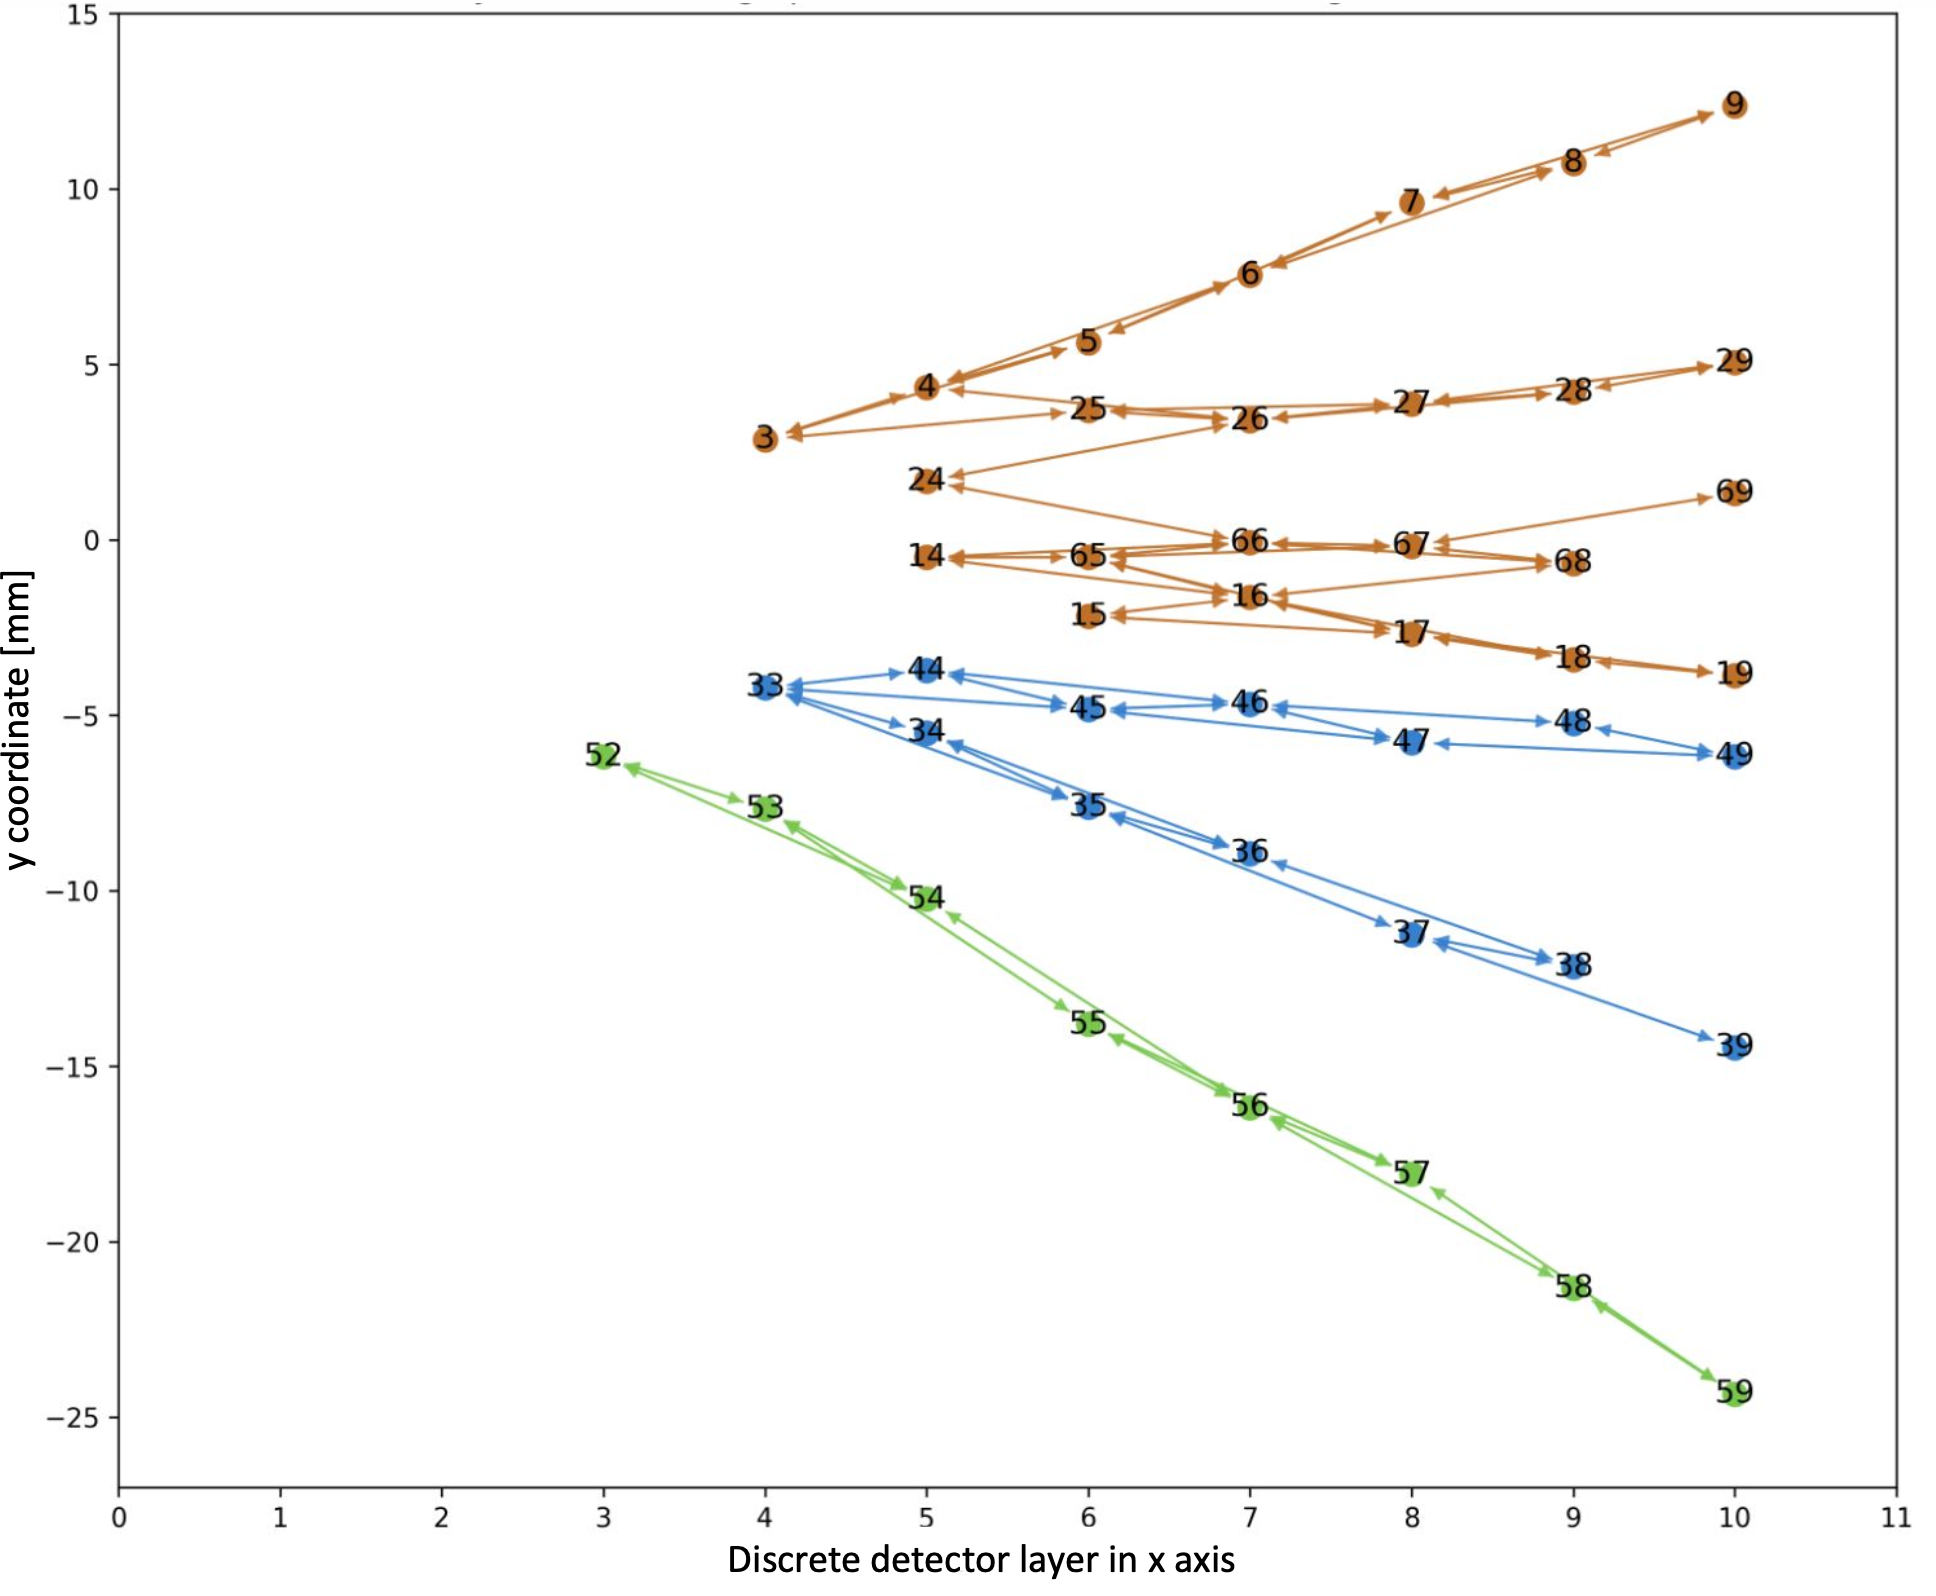
\includegraphics[width=10.7cm]{images/5-gnn-algorithm/mc-example-1.png} } \label{fig:mc-example-1}}%
    \hfill
    %\qquad
    \subfloat[\centering Extracted track candidates at each stage of the GNN algorithm]{{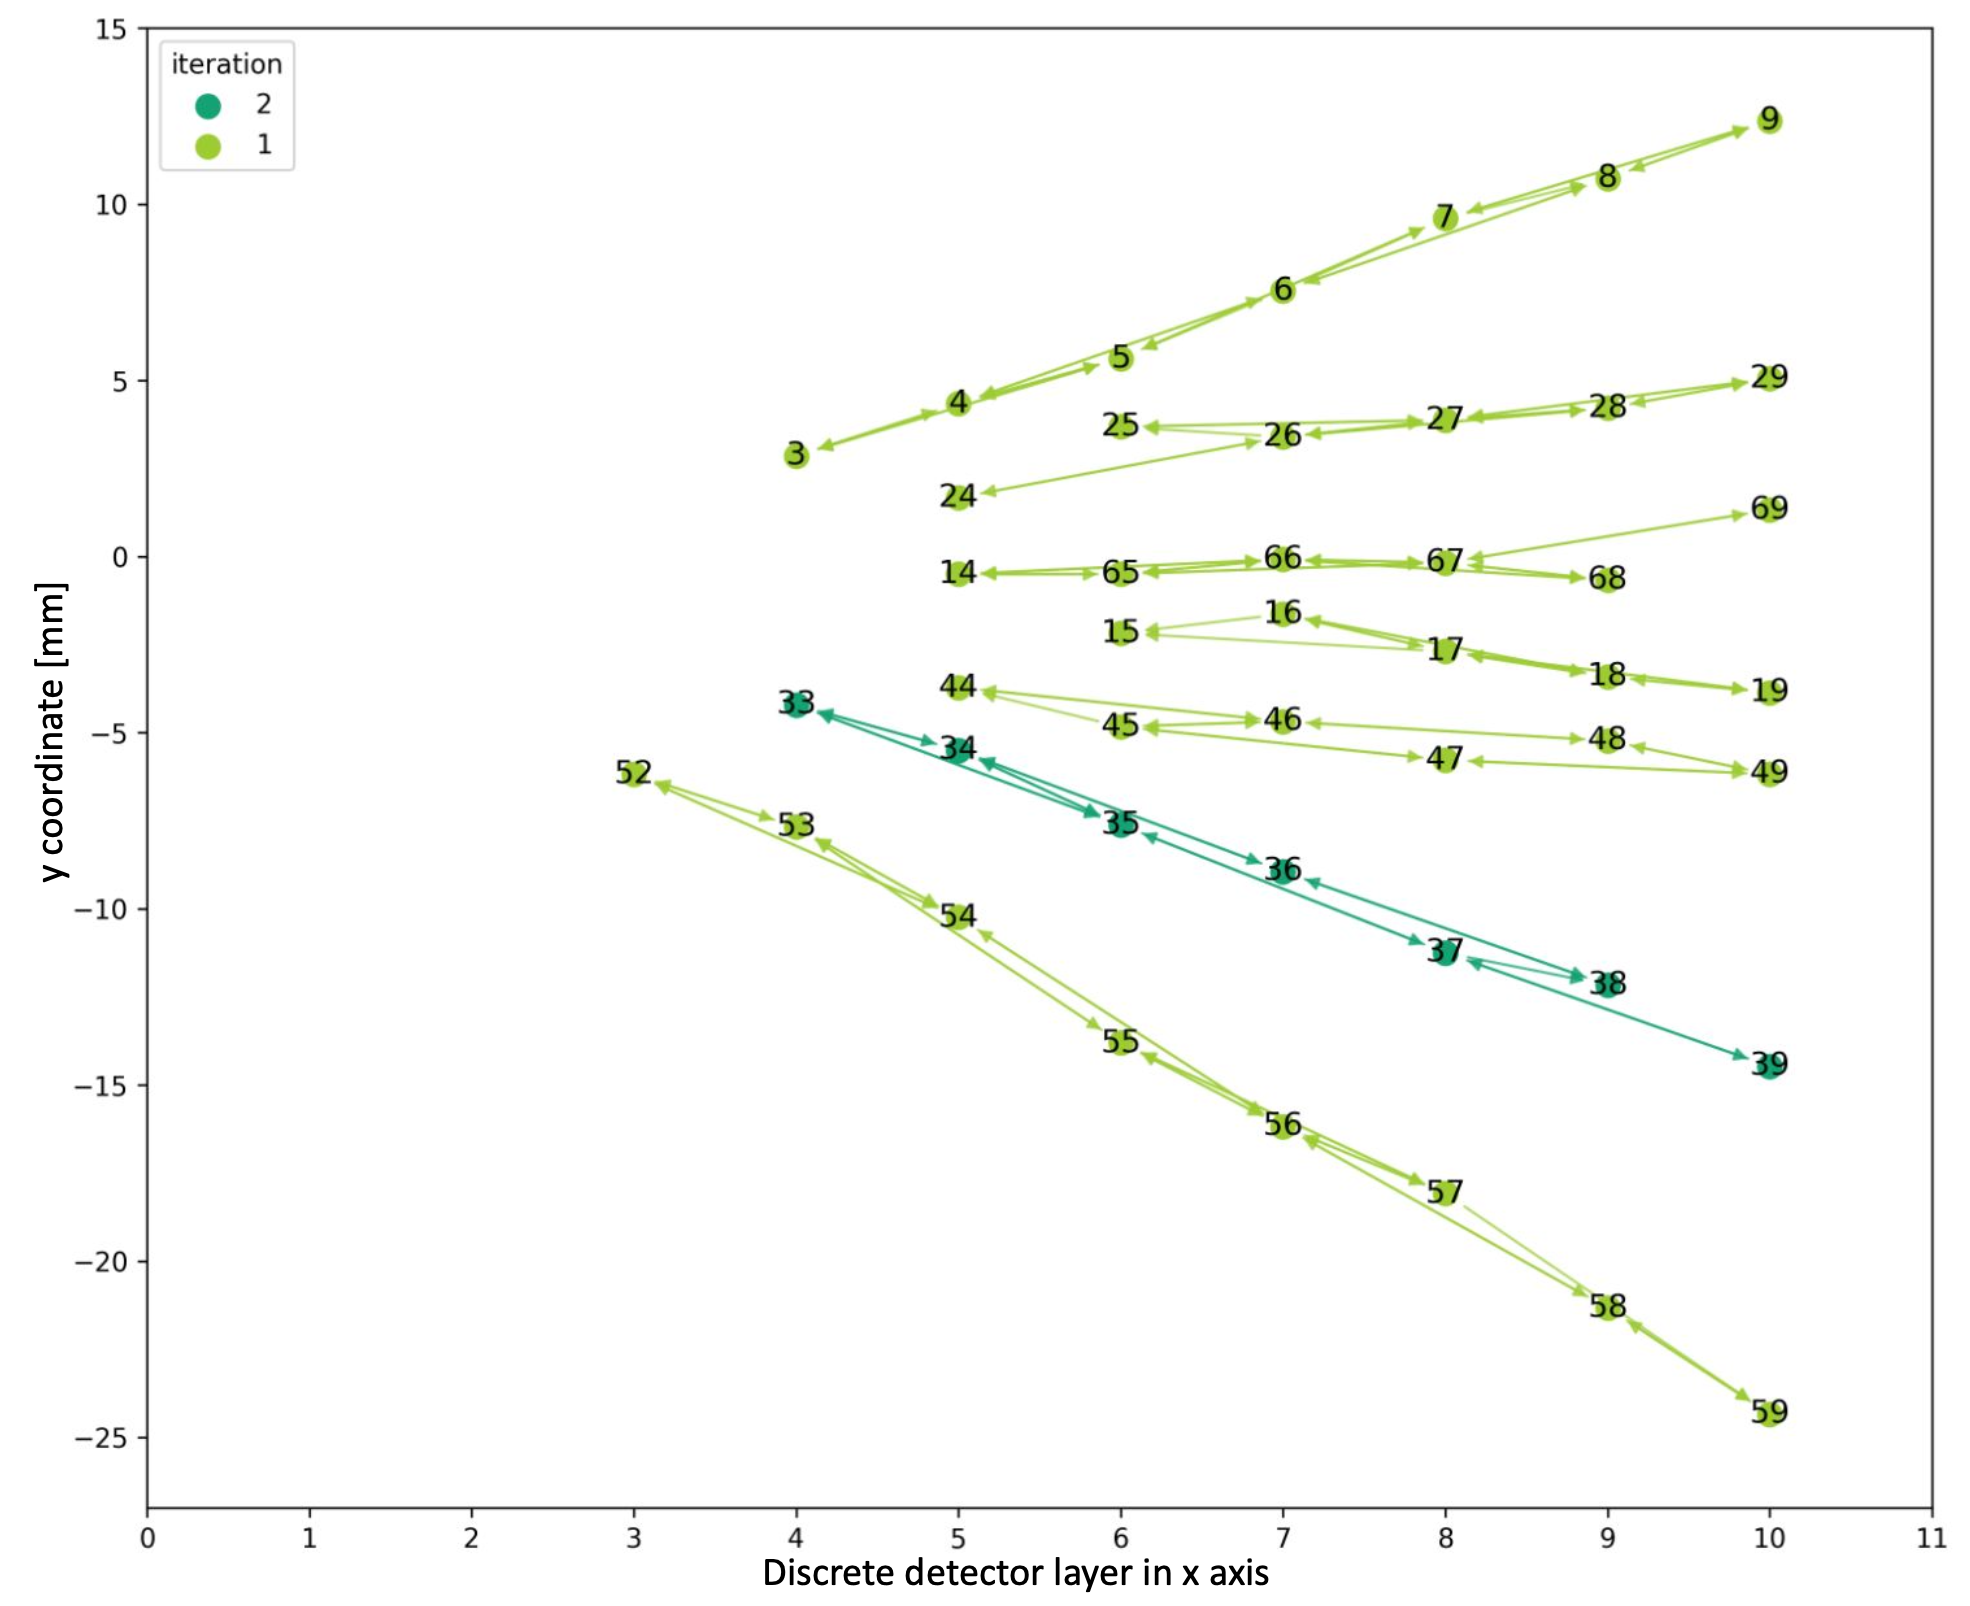
\includegraphics[width=11.1cm]{images/5-gnn-algorithm/mc-example-2.png} } \label{fig:mc-example-2}}%
    \caption{Results of the GNN-based algorithm applied to a simple MC simulation. a) The simulated graph network where nodes with $\sigma_e^2 > 0.8$ are not plotted as clustering was not possible for these nodes. A CCA was applied to split the graph network into smaller subgraphs, where each colour indicates a different subgraph. b) The extracted track candidates after the applied GMR and Information Aggregation stages, where seven separate track candidates can be seen.}%
    \label{fig:example-application-1}%
\end{figure}
%\end{center}

%\begin{center}
\begin{figure}[htbp]%
    \centering
    \subfloat[\centering Simulated graph network post CCA]{{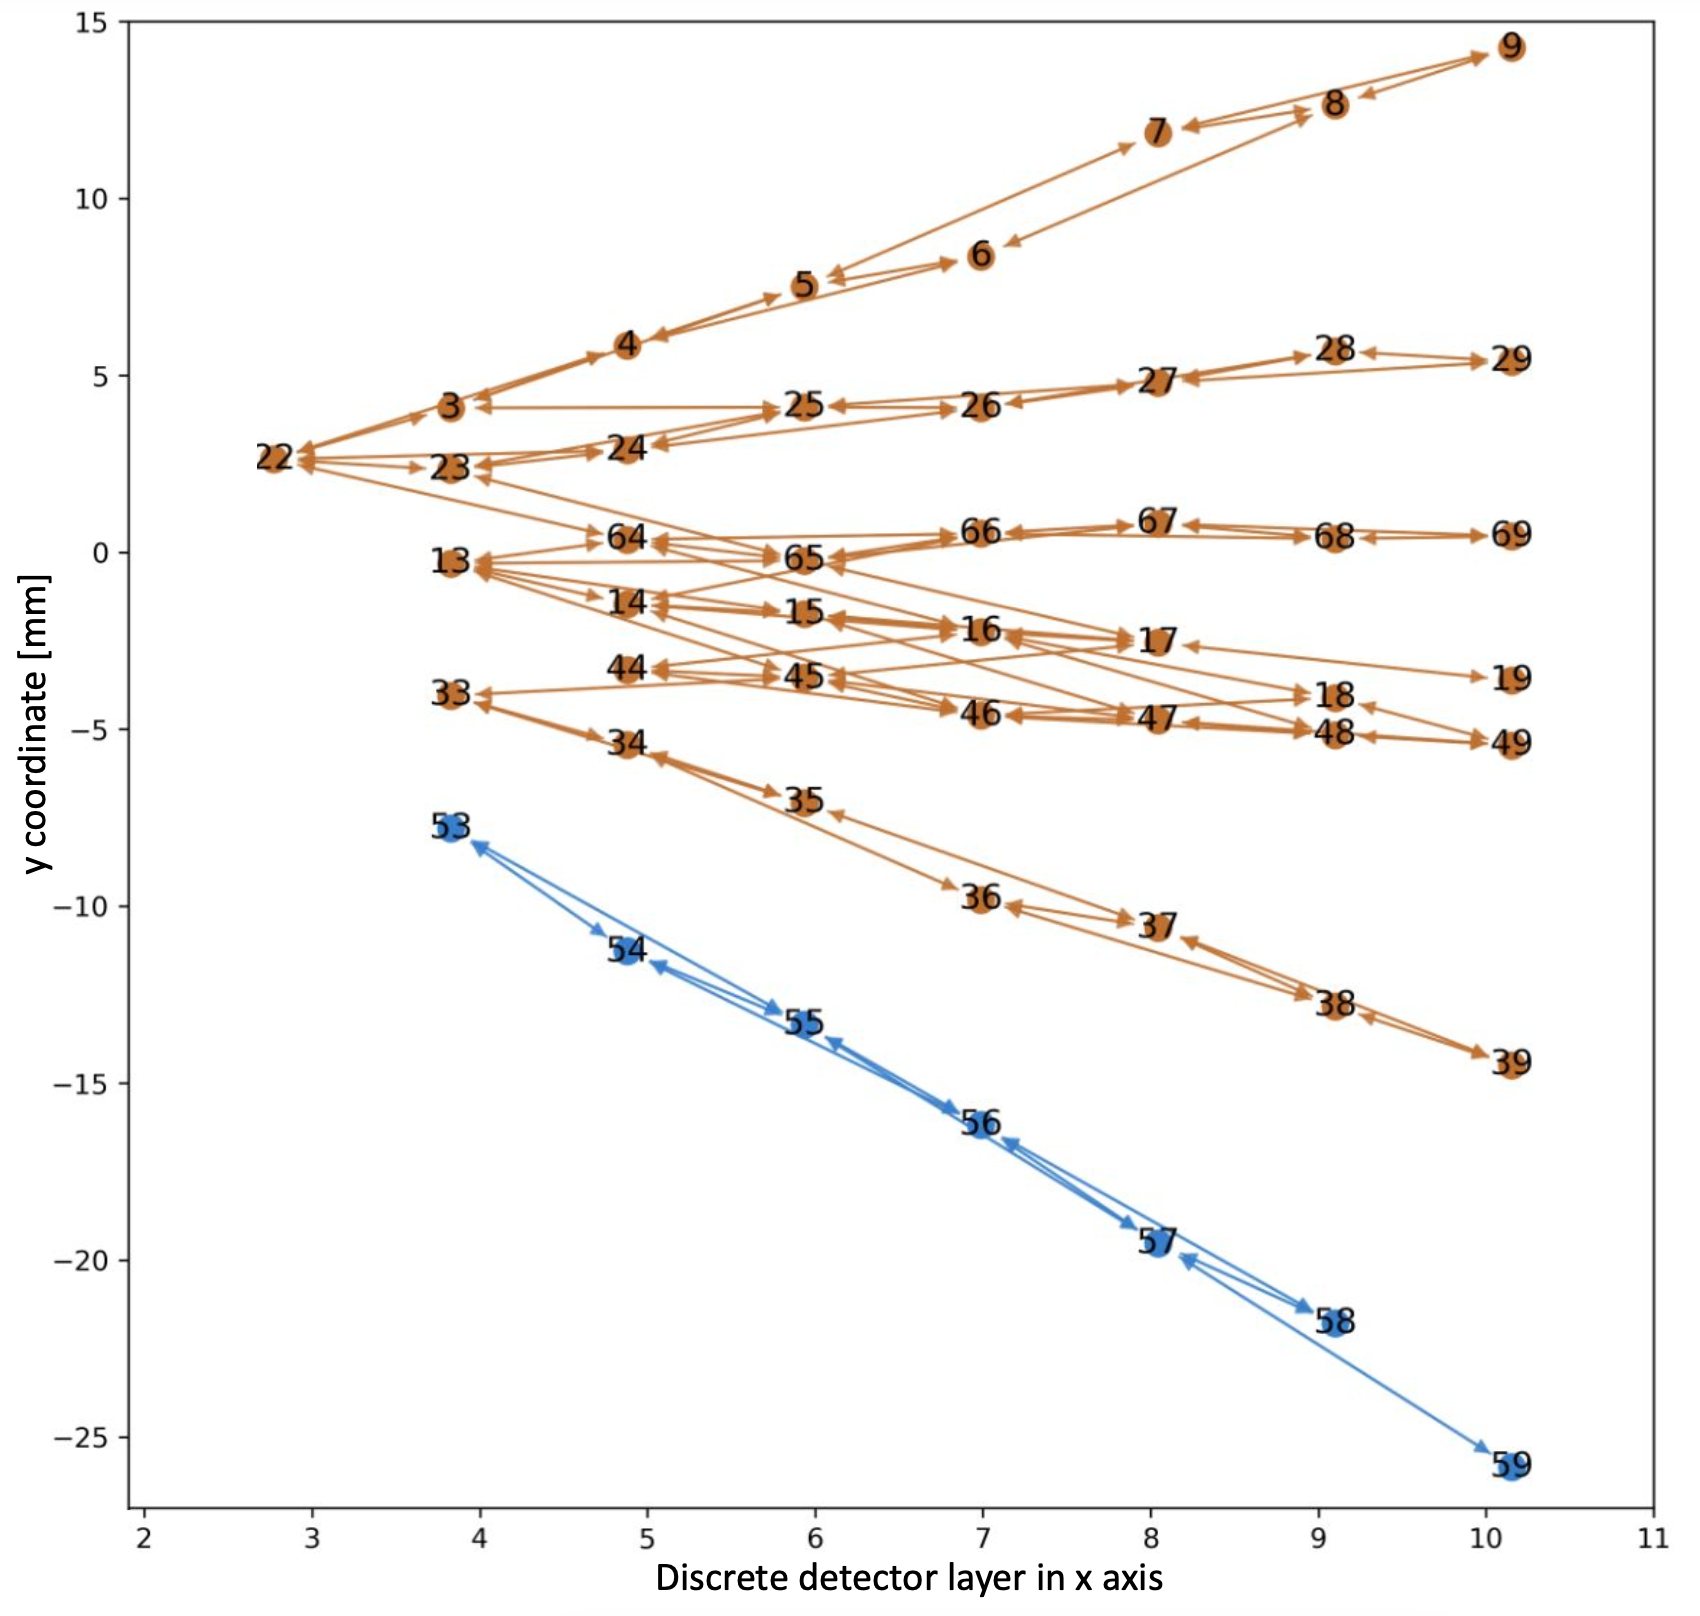
\includegraphics[width=9.8cm]{images/5-gnn-algorithm/mc-example-3.png} } \label{fig:mc-example-3}}%
    \hfill
    %\qquad
    \subfloat[\centering Extracted track candidates after stage 1]{{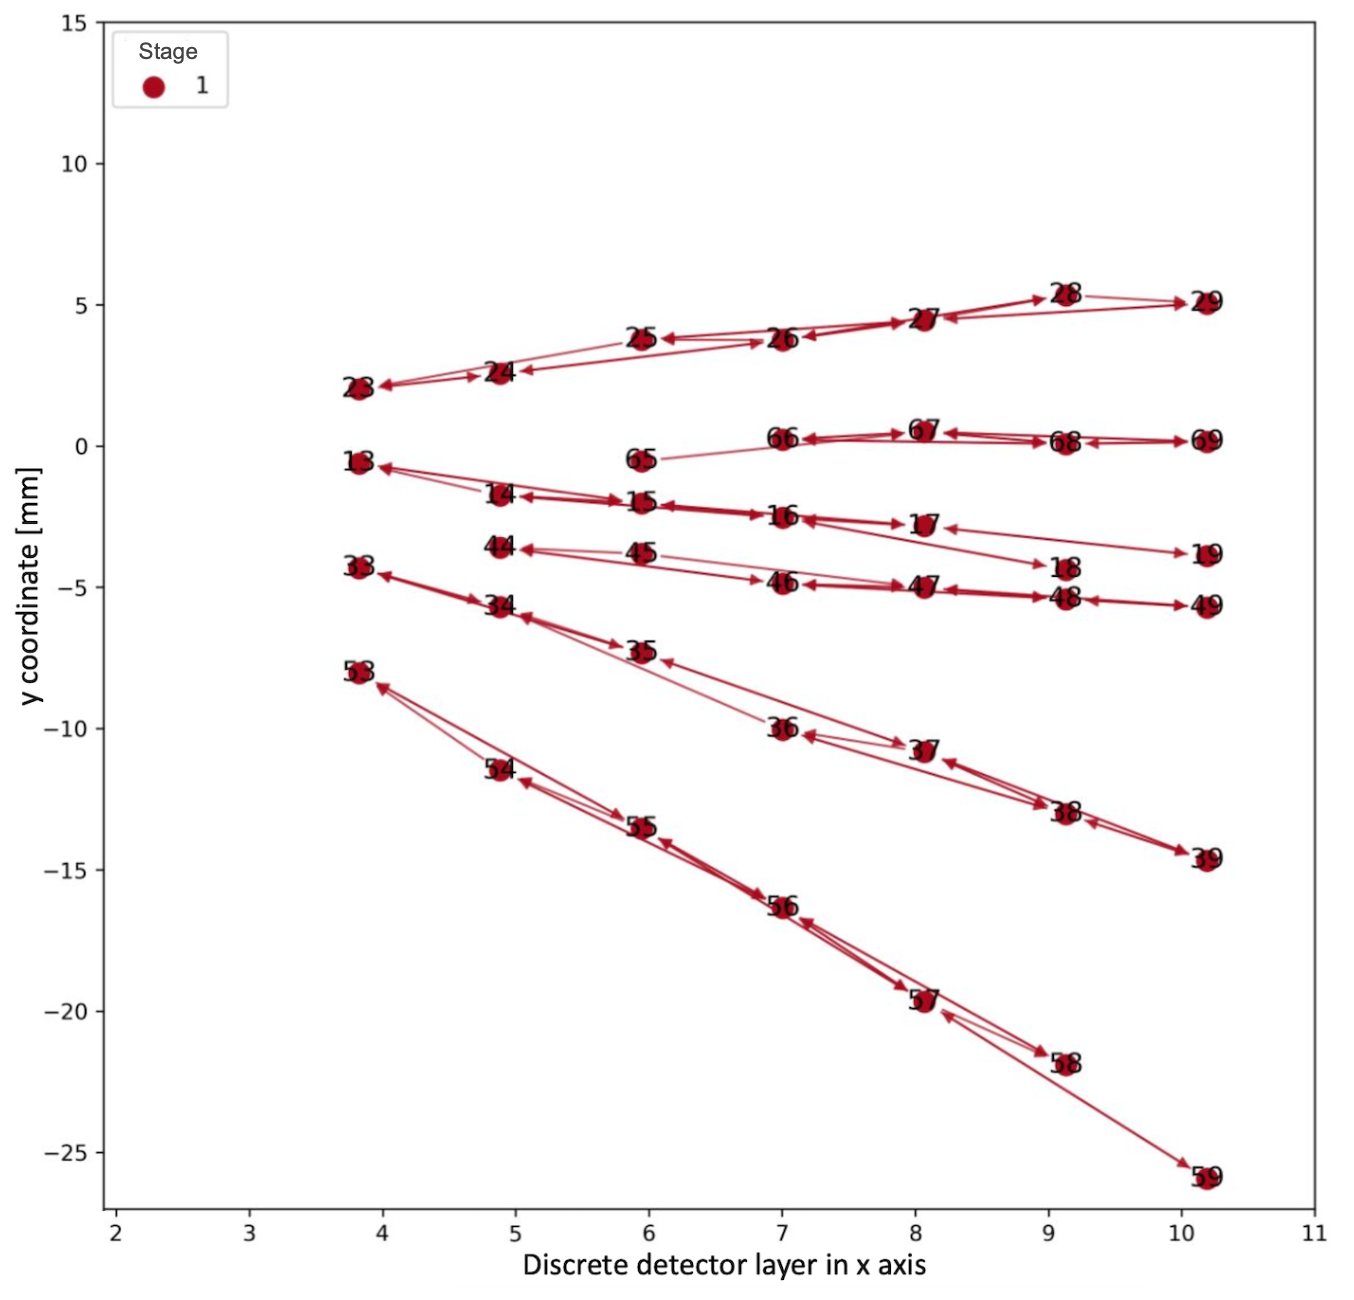
\includegraphics[width=10cm]{images/5-gnn-algorithm/mc-example-5.png} } \label{fig:mc-example-4}}%
    \caption{Results of the GNN-based algorithm applied to a simple MC simulation a) The simulated graph network where nodes with $\sigma_e^2 > 0.8$ are not plotted as clustering was not possible. A CCA was applied to split the graph network into smaller subgraphs, where each colour indicates a different subgraph. c) Six extracted track candidates after the GMR stage.}%
    \label{fig:example-application-2}%
\end{figure}
%\end{center}


\section{Conclusion}

The proposed GNN algorithm is successful in iteratively identifying outlier edge connections and extracting track candidates for simple simulated particle collision events. GMR via clustering of state vectors proves to be a successful first step towards resolving incompatible connections in the network. The KF works well for both the extrapolation of state vectors to neighbour nodes, as well as for track extraction and track fitting. This ensures neighbourhood information, can be aggregated in order to improve the precision in track state parameters. An intrinsic characteristic of the GNN algorithm is that neighbourhood complexity is inferred by the network. This is observed as the GNN algorithm automatically initiates the pattern recognition process in regions where outlier connections are easily identifiable. The network starts with low density regions and gradually progresses towards high density areas. This indicates that the GNN algorithm behaves as expected, first resolving ambiguities in ``cold'' regions and shows great promise for extraction of track candidates in more complex cases and realistic detector setups.


%---------------------------------------------
%	6. Application & Perform of GNN Algorithm
%---------------------------------------------

%\chapter{Application and Performance of GNN Algorithm}\label{chapter-6}

%The main application of the GNN algorithm on the trackML data, the data preparation, what data was exactly used and why, the ML classification algorithm used to build the edge connections. The main results we get from application of this algorithm, the track reconstruction efficiency, the purity metrics, computational performance. Comparison with other algorithms.

%nips-2018-competation
%Data.
%We used the fast (10s per event) and accurate simulation engine ACTS4 [6] to generate the challenge data. It allowed us to generate realistic data emulating a full Silicon LHC detector (see Fig 3), while providing us with the ground truth of particle trajectory membership. Thus, for each event we obtained the “detected” 3D points coordinates (and additional features), and, as ground truth, the list of points associated to each track. There is a one to one relationship between the true 3D points and the reconstructed ones.


\chapter{Application of the GNN Algorithm on the TrackML Model}
\label{chapter-6}

% This chapter focuses on the track finding algorithm development and its application on the publicly available dataset designed for the Kaggle TrackML challenge. The preliminary results related to track reconstruction efficiency and purity metrics are presented and discussed.

%The main application of the GNN algorithm on the trackML data, the data preparation, what data was exactly used and why, the ML classification algorithm used to build the edge connections. The main results we get from application of this algorithm, the track reconstruction efficiency, the purity metrics, computational performance. Comparison with other algorithms.


\section{Implementation}


\subsection{Data Preparation}
%Talk specifically about the TrackML data here and how it was prepared. How the trackml hits are converted into nodes and edges. Close proximity node merging. Checks that are put in place in order to make sure there are no hits that have the same module id (more than 2 hits that are simultaneously in the same module and volume and layer).



\subsection{Constructing Track State Estimates}
\label{constructing-track-states}

Track parameters in both the transverse $x$-$y$ plane and the $r$-$z$ plane are considered in order to construct track state estimates $X_{ij}$.


\subsubsection{Parabolic Model}
\label{parabolic-state}

In the $x$-$y$ plane, charged particles experience the influence of the magnetic field, so naturally their trajectories follow a near-parabolic shape. For a given node A, a parabola is formed using the origin O, node A and neighbour node B, illustrated in Figure \ref{fig:gnn-parabolic-model}. The parabola is transformed into the local coordinate system of node A such that the new $x$-axis, $X_A$ goes through the global origin O and node A. The parabolic parameters \{$a, b, c$\} are computed using equations Eq \eqref{eqn:parabolic-equations}. The measurement vector $[m_O \quad m_A \quad m_C]$ is obtained in the coordinate system local to node A, assuming $m_O = 0$ and $m_A = 0$.

\begin{equation}
\begin{aligned}
m_O = ax_{O}^{2} + bx_O + c \\
m_A = c \\
m_B = ax_{B}^{2} + bx_B + c
\end{aligned}
\label{eqn:parabolic-equations}
\end{equation}

\begin{figure}[htbp!] 
    \centering
    \subfloat[]{%
        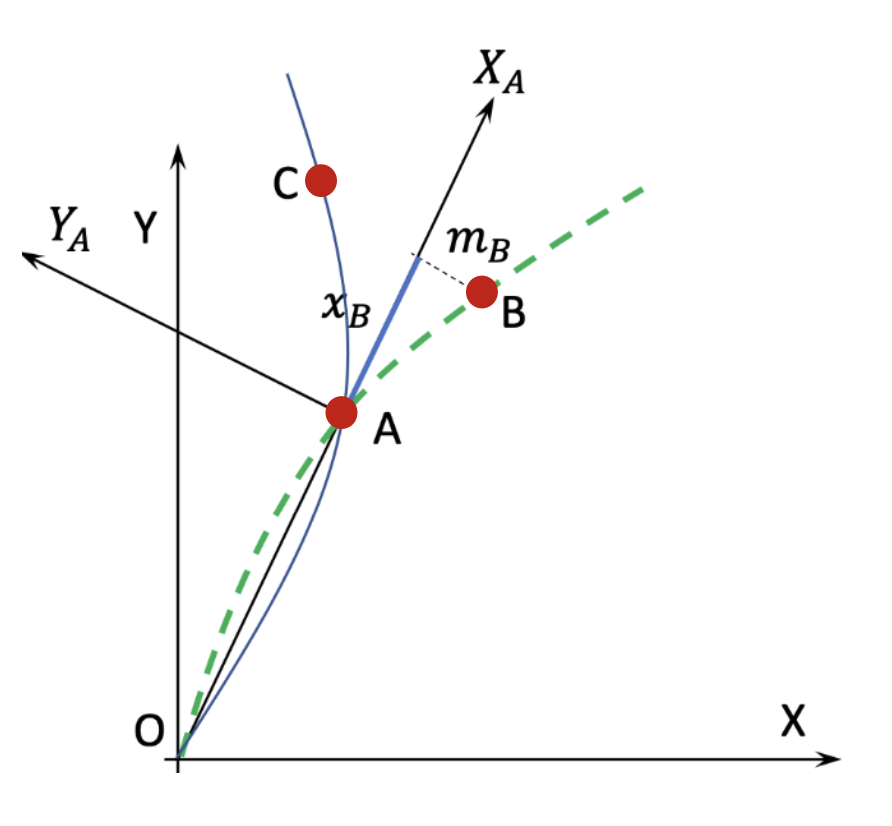
\includegraphics[width=0.43\textwidth]{images/5-gnn-algorithm/parabolic-state-model-1.png}%
        \label{fig:gnn-parabolic-state-1}%
        }%
    \hfill%
    \subfloat[]{%
        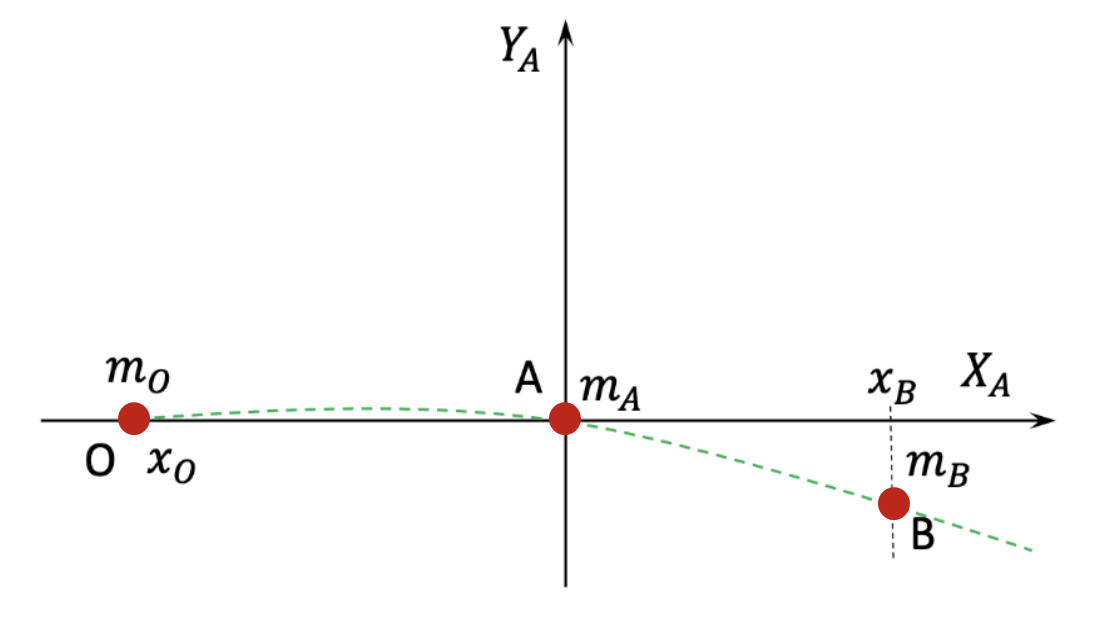
\includegraphics[width=0.57\textwidth]{images/5-gnn-algorithm/parabolic-state-model-2.png}%
        \label{fig:gnn-parabolic-state-2}%
        }%
    \caption{Illustrations of the parabolic model used in the $x$-$y$ plane. a) shows the construction of a parabola between the global origin, O and nodes A - B, as well as a second parabola between O - A - C. b) shows the rotation of the parabola O - A - B into the local coordinate system of node A.}
    \label{fig:gnn-parabolic-model}
\end{figure}


\subsubsection{Linear Model}
\label{linear-state}

The $r$-$z$ plane is parallel to the direction of travel of the beamline, where tracks follow a linear model. The inverse track inclination between a node and its neighbour, $\tau$, is used and is given by Eq \eqref{eqn:tau-parameter}, where $z_A$, $r_A$ refer to measurements of the node and $z_B$, $r_B$ refer to measurements of its neighbour. $r$ is the square root of the sum in quadrature of the $x$ and $y$ measurements.

\begin{equation}
\tau = \frac{z_A - z_B}{r_A - r_B}
\label{eqn:tau-parameter}
\end{equation}

\subsubsection{Track State Estimate}

Parabolic parameters $a$ and $b$ in the $x$-$y$ plane, as well as inverse track inclination $\tau$ in the $r$-$z$ plane give an indication of track orientation. For node $i$ and its neighbour $j$, the track state estimate $X_{ij}$ is given by Eq \eqref{eqn:joint-state-vector}

\begin{equation}
X_{ij} = \begin{bmatrix} a \\ b \\ \tau \end{bmatrix}
\label{eqn:joint-state-vector}
\end{equation}






\subsection{Derivation of Covariance}

\subsection{Moliere Theory of Multiple Scattering}
\begin{itemize}
\item highland formula and handling the error/effects due to multiple scattering for the barrel and endcap in slightly different ways
\item how were the covariances dervied and the sigma errors chosen
\item Derivation of the edge state covariance
\item 2 different ones, we start with the edge covariance, and derive the state covariance
\end{itemize}
% moliere theory links:
%https://gray.mgh.harvard.edu/attachments/article/337/Techniques%20of%20Proton%20Radiotherapy%20(06)%20Multiple%20Scattering.pdf
%https://pdg.lbl.gov/2005/reviews/passagerpp.pdf





\subsection{Determining the Optimal KL Threshold}
\label{chapter-6-kl-threshold}

If $d_{KL}$ $\leq$ some threshold, then states can be clustered together and merged into a single state.

To determine the optimal pairwise $d_{KL}$ between track state estimates $X_{ij}$ for a given node, a SVM classifier was trained using pairwise $d_{KL}$ and $\sigma_{e}$ as input features. A MC simulation of $10,000$ particle collision events, each event with ten truth tracks, was used to build a training dataset. Loosely compatible edge connections were formed using a hit-pair predictor based on track inclination angle of neighbouring hits. The feature vector was comprised of $\sigma_{e}$ for a given node, and pairwise $d_{KL}$ between track states. The ground truth particle was extracted for each pairwise connection, where truth 1 corresponded to hits from both track states originating from the same truth particle, and truth 0 otherwise. A SVM was trained to discriminate between the two classes \cite{scikit-learn}, using a polynomial degree three kernel. Predictions were adjusted such that the TPR was tuned to 95\% and the decision boundary was converted into a fast LUT using a similar methodology outlined in Section \ref{LUT-generation}.  Other classification algorithms were explored, however the SVM was the most appropriate in this instance to determine a decision boundary to best separate the classes.

\begin{figure}[htbp!] 
    \centering
    \subfloat[]{%
        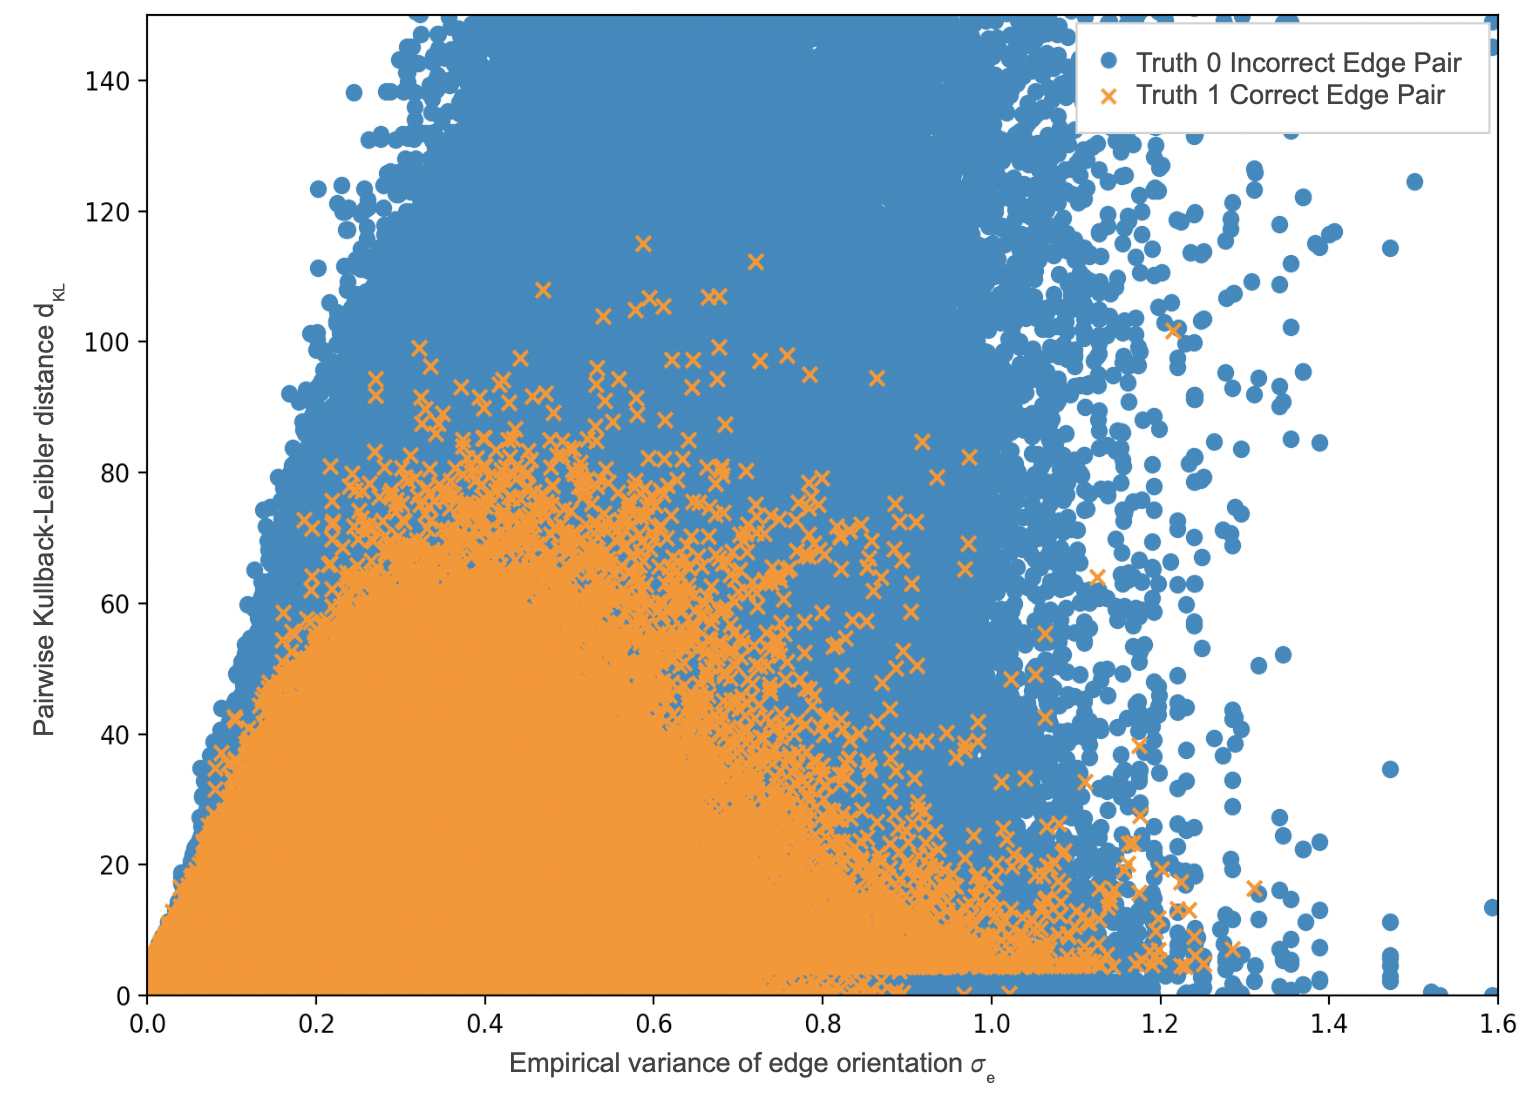
\includegraphics[width=0.8\linewidth]{images/6-results/kl-truth.png}%
        \label{fig:KL-distance-truth}%
        }%
    \hfill%
    \subfloat[]{%
        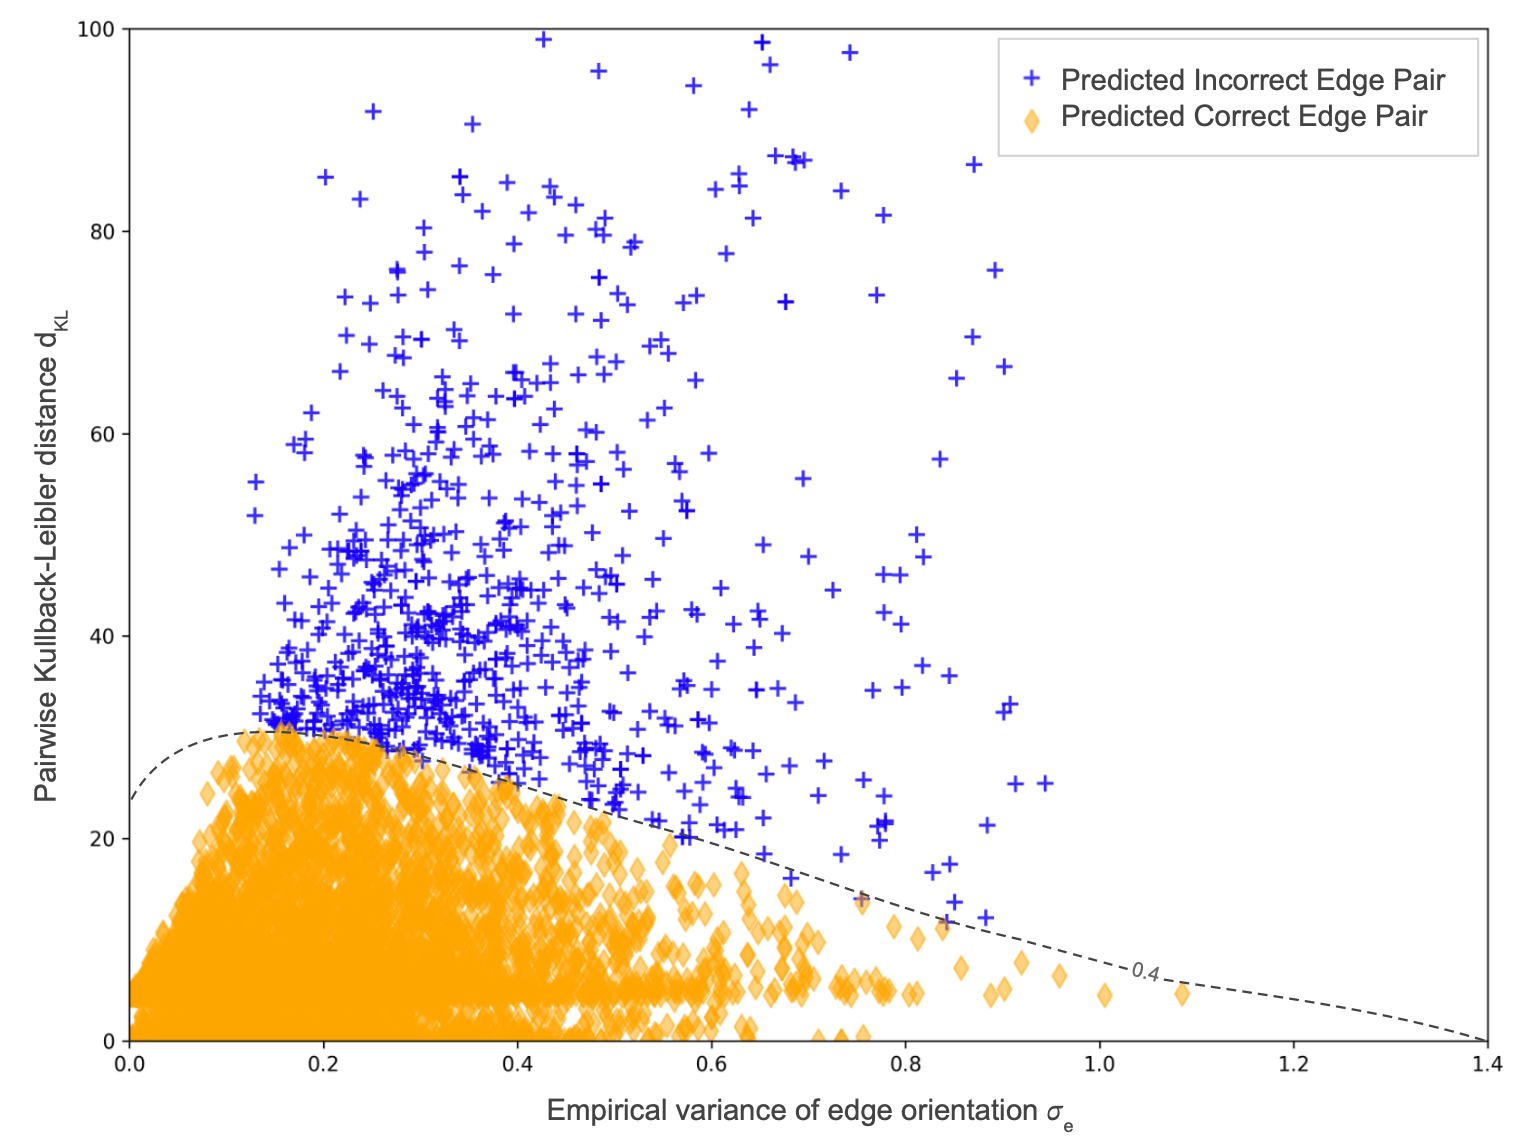
\includegraphics[width=0.8\linewidth]{images/6-results/kl-predictions.png}%
        \label{fig:KL-distance-predictions}%
        }%
    \caption{}
    \label{fig:KL-distance}
\end{figure}





\subsection{Extrapolation Models}
\label{chapter-6-extrapolation}
\subsubsection{Linear Extrapolation Model}
\subsubsection{Parabolic Extrapolation Model}
\begin{itemize}
    \item Information propagation via Message Passing Mechanism
    \item Extrapolation and Validation
    \item Linear and Parabolic model - 2 different extrapolations for xy componenets of state vector and rz componenet, illustrations here
    \item Kalman Filter Update, OU process for correlated noise
\end{itemize}

Mention here that both the linear and parabolic models were used in this instance, where the track state estimate comprised of a 3x1 vector, a, b, tau. The extrapolation and KF update will be different here, different transition Jacobian matrix. Also mention about tuning the chi2 distance thresholds during extrapolation

%The matrix $\widetilde{C}_{ij}$ includes the addition of the process noise $Q$ modelled by the Ornstein-Uhlenbeck (OU) process \cite{OU} which encompasses all material effects. See Section \ref{kf} for further details. The full derivation of $F$ and $Q$ are shown in Appendix \ref{appendix:Appendix-A}


\subsection{Implementation of Kalman Filters}
\label{gnn-kf-implementation}
Mention about the OU process noise, for correlated noise etc

%\begin{itemize}
%\item emphasis on the use of KFs both in information aggregation stage and in track extraction, both are implemented in different ways, is a useful and unique part to this algorithm
%\item OU process noise
%\end{itemize}



\section{Endcap Results and Performance Evaluation}

% track purity, particle purity, track reconstruction efficiency
% TODO: mention here that the parabolic track state model was used and the joint track state was used, and mention the section here

%nips-2018-competation
%Data.
%We used the fast (10s per event) and accurate simulation engine ACTS4 [6] to generate the challenge data. It allowed us to generate realistic data emulating a full Silicon LHC detector (see Fig 3), while providing us with the ground truth of particle trajectory membership. Thus, for each event we obtained the “detected” 3D points coordinates (and additional features), and, as ground truth, the list of points associated to each track. There is a one to one relationship between the true 3D points and the reconstructed ones.

%\begin{itemize}
%    \item Application on TrackML model, endcap volume only, metrics, performance eval etc, track reconstruction efficiency, track purity and particle purity, comparison with TrackML solutions
%    \item Track reconstruction efficiency, track purity, particle purity
%    \item Performance Evaluation
%    \item execution time?
%\end{itemize}


\section{Outlook}
\subsection{Extension to the Barrel Region}
\subsection{Software Optimisations}

\subsection{Other Approaches}
\subsubsection{Community Detection}
\subsubsection{Cellular Automatons}

%If a subgraph does not meet the criteria to qualify as a good track candidate, a \textit{Community Detection} algorithm \cite{community} is applied in order to further partition the set of nodes. Community Detection is a generalisation of CCA and works by using a distance metric, typically modularity, in order to label nodes as \textit{closely connected}. Modularity is a benefit function that measures the strength of a particular division of a network using the number of edges. A popular modularity maximisation approach is the Louvain method \cite{python_louvain}, which iteratively optimises local communities until global modularity can no longer be improved. An example illustration of a network partition via Community Detection is shown in Figure \ref{fig:community-detection}. Any subgraphs with zero extracted candidates through this procedure are propagated to further stages for additional processing.

%Community Detection: divides nodes into various clusters based on edge structure. It learns from edge weights, and distance and graph objects similarly. 

%\begin{figure}[htbp]
%    \centering
%    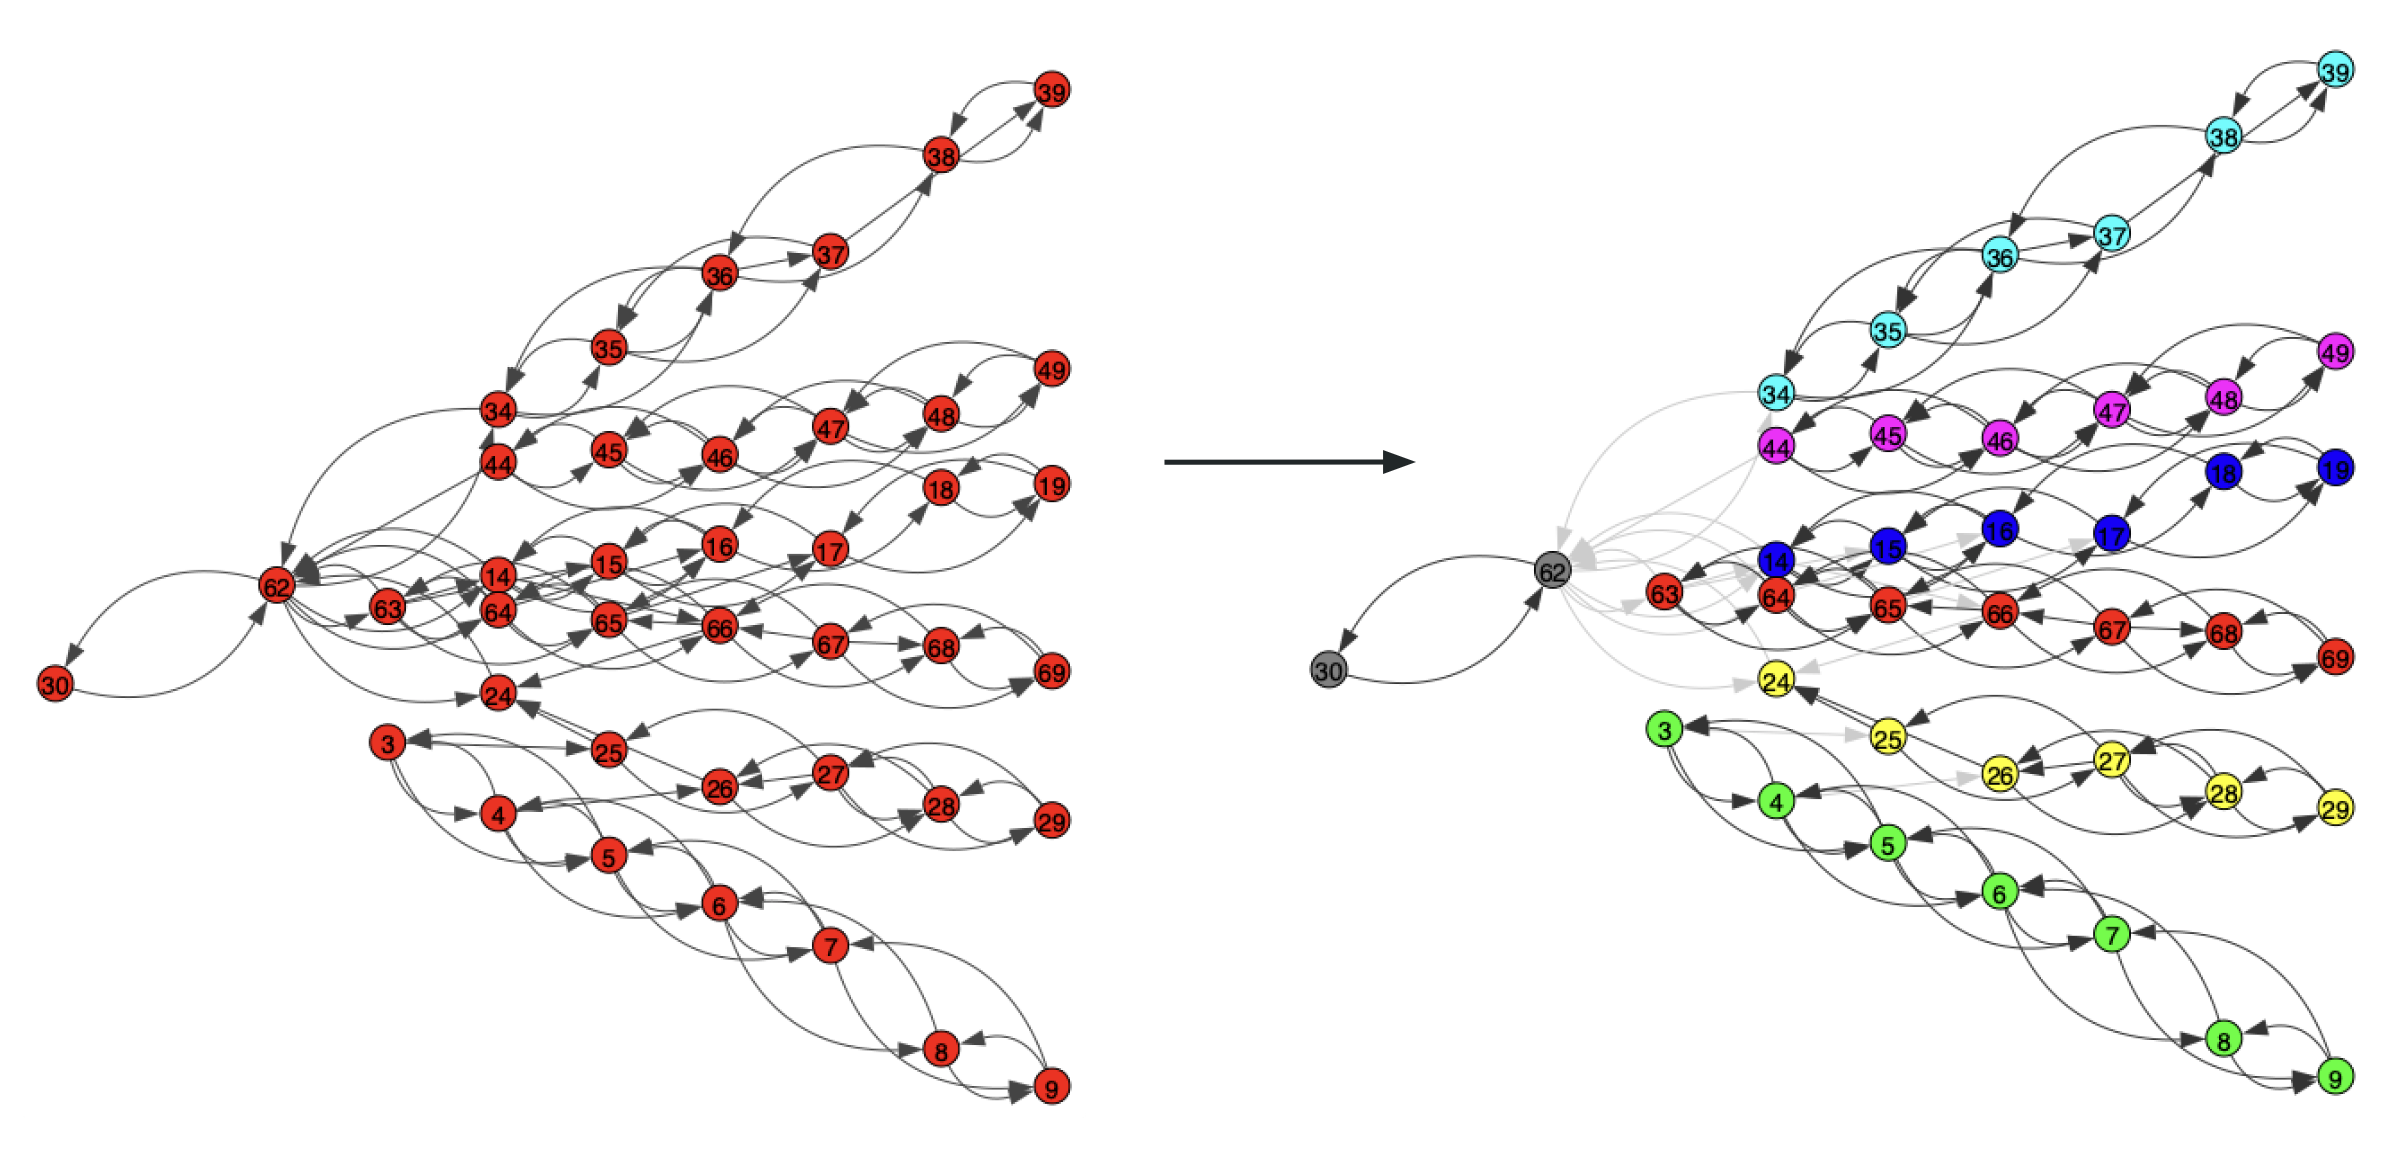
\includegraphics[width=0.98\textwidth]{images/5-gnn-algorithm/community-detection.png}
%    \caption{TODO: caption ....}
%    \label{fig:community-detection}%
%\end{figure}

%\begin{itemize}
%    \item extension to barrel, analysis of results, performance  evaluation, challenges and outlook
%    \item Optimisation - GPU acceleration etc
%\end{itemize}


\section{Conclusions}
%------------------------------------
%	7. Summary & Outlook
%------------------------------------


\chapter{Summary and Outlook}



\newpage
\empty


%---------------------
%	List of Figures
%---------------------
\addcontentsline{toc}{chapter}{List of Figures}
\listoffigures


%---------------------
%	List of Tables
%---------------------
\newpage
\addcontentsline{toc}{chapter}{List of Tables}
\listoftables


%---------------------
%	BIBLIOGRAPHY
%---------------------
\addcontentsline{toc}{chapter}{References}
% \bibliographystyle{unsrt}
\bibliographystyle{bibliography/JHEP}
\bibliography{bibliography/LHC-ATLAS}


\end{document}